\documentclass[12pt,a4paper,bibliography=totocnumbered,listof=totocnumbered]{scrartcl}
% u.U. muss Koma-Skript Package ueber MikTeX deinstalliert und neu installiert werden
% Hilft das nicht, so sollte statt scrartcl die Dokumentenklasse article verwendet werden
\usepackage[backend=bibtex,sorting=none,style=alphabetic]{biblatex}
\usepackage[ngerman]{babel}
\usepackage[utf8]{inputenc}
\usepackage{ifthen}
\usepackage{xargs}
\usepackage{amsmath}
\usepackage{amsfonts}
\usepackage{amssymb}
\usepackage{graphicx}
\usepackage{fancyhdr}
\usepackage{tabularx}
\usepackage{geometry}
\usepackage{setspace}
\usepackage[right]{eurosym}
\usepackage[printonlyused]{acronym}
\usepackage{subfig}
\usepackage{floatflt}
\usepackage{float}
\usepackage[usenames,dvipsnames]{color}
\usepackage{colortbl}
\usepackage{paralist}
\usepackage{array}
\usepackage{titlesec}
\usepackage{parskip}
\usepackage[right]{eurosym}
\usepackage[subfigure,titles]{tocloft}
\usepackage[pdfpagelabels=true]{hyperref}

\usepackage{listings}
\lstset{basicstyle=\footnotesize, captionpos=b, breaklines=true, showstringspaces=false, tabsize=2, frame=lines, numbers=left, numberstyle=\tiny, xleftmargin=2em, framexleftmargin=2em}
\makeatletter
\def\l@lstlisting#1#2{\@dottedtocline{1}{0em}{1em}{\hspace{1,5em} Lst. #1}{#2}}
\makeatother






%%%%%%%%%%%%%%%%%%%%%%%%%%%%%%%%%%%%%%%%%%%%%%%%%%%%%%%%%%%%%%%
%% JSON Listings
%
%\usepackage{bera}% optional: just to have a nice mono-spaced font
%\usepackage{chngcntr} 
%\usepackage{listings}
%\usepackage{xcolor}
%
%\definecolor{background}{HTML}{EEEEEE}
%\definecolor{delim}{RGB}{20,105,176}
%\definecolor{identifier}{RGB}{152,092,173}
%\definecolor{textValue}{RGB}{233,133,078}
%\definecolor{numb}{RGB}{109,134,000}
%\definecolor{black}{RGB}{0,0,0}
%
%\lstdefinelanguage{json}{
%    %basicstyle=\normalfont\ttfamily,
%    numbers=none,
%    numberstyle=\scriptsize,
%    stepnumber=1,
%    numbersep=8pt,
%    showstringspaces=false,
%    breaklines=true,
%    frame=lines,
%    backgroundcolor=\color{background},
%    literate=
%     *{Size}{{{\color{identifier}Size}}}{4}
%      {x}{{{\color{identifier}x}}}{1}
%      {y}{{{\color{identifier}y}}}{1}
%      {SpawnPosition}{{{\color{identifier}SpawnPosition}}}{14}
%      {Position}{{{\color{identifier}Position}}}{8}
%      {Enemies}{{{\color{identifier}Enemies}}}{7}
%      {Type}{{{\color{identifier}Type}}}{4}
%      {Rotation}{{{\color{identifier}Rotation}}}{8}
%      {Amount}{{{\color{identifier}Amount}}}{6}
%      {BASIC}{{{\color{numb}BASIC}}}{5}
%      {PISTOL}{{{\color{numb}PISTOL}}}{6}
%      {Doors}{{{\color{identifier}Doors}}}{5}
%      {HORIZONTAL}{{{\color{numb}HORIZONTAL}}}{10}
%      {LevelItems}{{{\color{identifier}LevelItems}}}{10}
%      {Weapons}{{{\color{identifier}Weapons}}}{7}
%      {Walls}{{{\color{identifier}Walls}}}{5}
%      {MACHINEGUN}{{{\color{numb}MACHINEGUN}}}{10}
%      {PatrolPoints}{{{\color{identifier}PatrolPoints}}}{12}
%      {ActualPosition}{{{\color{identifier}ActualPosition}}}{14}
%      {LevelElements}{{{\color{identifier}LevelElements}}}{14}
%      {LeftClasperPoint}{{{\color{textValue}LeftClasperPoint}}}{16}
%      {WeaponType}{{{\color{identifier}WeaponType}}}{10}
%      {tool2}{{{\color{textValue}tool2}}}{5}
%      {0}{{{\color{numb}0}}}{1}
%      {1}{{{\color{numb}1}}}{1}
%      {2}{{{\color{numb}2}}}{1}
%      {3}{{{\color{numb}3}}}{1}
%      {4}{{{\color{numb}4}}}{1}
%      {5}{{{\color{numb}5}}}{1}
%      {6}{{{\color{numb}6}}}{1}
%      {7}{{{\color{numb}7}}}{1}
%      {8}{{{\color{numb}8}}}{1}
%      {9}{{{\color{numb}9}}}{1}
%      {:}{{{\color{black}{:}}}}{1}
%      {,}{{{\color{black}{,}}}}{1}
%      {\{}{{{\color{delim}{\{}}}}{1}
%      {\}}{{{\color{delim}{\}}}}}{1}
%      {[}{{{\color{delim}{[}}}}{1}
%      {]}{{{\color{delim}{]}}}}{1},
%}
%%%%%%%%%%%%%%% End Listing. %%%%%%%%%%%%%%%%%%%%%







\geometry{a4paper, top=27mm, left=20mm, right=20mm, bottom=35mm, headsep=10mm, footskip=12mm}

\definecolor{javared}{rgb}{0.6,0,0} % for strings
\definecolor{javagreen}{rgb}{0.25,0.5,0.35} % comments
\definecolor{javapurple}{rgb}{0.5,0,0.35} % keywords
\definecolor{javadocblue}{rgb}{0.25,0.35,0.75} % javadoc
\definecolor{gray}{rgb}{0.6,0.6,0.6}
 
\lstset{language=Java,
basicstyle=\ttfamily\footnotesize,
keywordstyle=\color{javapurple}\bfseries,
stringstyle=\color{javared},
commentstyle=\color{javagreen}\itshape\bfseries,
morecomment=[s][\color{javadocblue}]{/**}{*/},
numbers=left,
numberstyle=\tiny\color{gray},
stepnumber=1,
numbersep=10pt,
tabsize=3,
showspaces=false,
showstringspaces=false}
\titlespacing{\section}{0pt}{12pt plus 4pt minus 2pt}{-6pt plus 2pt minus 2pt}

% Kopf- und Fusszeile
\renewcommand{\sectionmark}[1]{\markright{#1}}
\renewcommand{\leftmark}{\rightmark}
\pagestyle{fancy}
\lhead{}
\chead{}
\rhead{\thesection\space\contentsname}
\lfoot{}
\cfoot{}
\rfoot{\ \linebreak Seite \thepage}
\renewcommand{\headrulewidth}{0.4pt}
\renewcommand{\footrulewidth}{0.4pt}

% Vorspann
\renewcommand{\thesection}{\Roman{section}}
\renewcommand{\theHsection}{\Roman{section}}
\pagenumbering{Roman}

\newcommand{\folgen}[1]{
\ensuremath
#1
}

\newcommandx{\rueckert}[3][]{
	\def\nameRueckert{#1}%
	\def\matnrRueckert{#2}%
	\def\studiengangRueckert{#3}%
}

\newcommandx{\hiller}[3][]{
	\def\nameHiller{#1}%
	\def\matnrHiller{#2}%
	\def\studiengangHiller{#3}%
}

\newcommandx{\dunphy}[3][]{
	\def\nameDunphy{#1}%
	\def\matnrDunphy{#2}%
	\def\studiengangDunphy{#3}%
}

\newcommandx{\koch}[3][]{
	\def\nameKoch{#1}%
	\def\matnrKoch{#2}%
	\def\studiengangKoch{#3}%
}

\newcommandx{\MyTitelseite}[6][]{
\thispagestyle{empty}

\includegraphics[scale=0.2]{pics/oth-logo.png}\hfill
\begin{center}
\ifthenelse{\equal{#1}{2}}{ % then
	\vspace*{2cm}
	\Large
	\textbf{Ostbayerische Technische Hochschule Regensburg}\\
	\textbf{Fakultät für Informatik und Mathematik}\\
	\vspace*{2cm}
	\Huge
	\textbf{#2}\\[1em]
	\large
	Zur Erlangung des akademischen Grades des\\
	\ifthenelse{\equal{#2}{Bachelorarbeit}}{Bachelor of Science (B.Sc.)}{Master of Science (M.Sc.)}\\
	\vspace*{1cm}
	\Large
	\textbf{#3}\\
}{ % else
	\vspace*{1cm}
	\Large
	\textbf{#3}\\
	\vspace*{2cm}
	\large
	An der Fakultät für Informatik und Mathematik der\\
	Ostbayerischen Technischen Hochschule Regensburg\\[2em]
	eingereichter\\
	\vspace*{1cm}
	\Large
	\textbf{#2}\\[2em]
}
	\vfill
	\includegraphics[height=6cm]{#6}
	\vfill
	\normalsize
	%\newcolumntype{x}[1]{>{\raggedleft\arraybackslash\hspace{0pt}}p{#1}}
	\begin{tabular}{rlll}%{6cm}p{7.5cm}}
	    \rule{0mm}{1ex}\textbf{Teammitglieder:}
	    & \nameHiller & \matnrHiller & \studiengangHiller \\
	    & \nameRueckert & \matnrRueckert & \studiengangRueckert\\ 
		& \nameDunphy & \matnrDunphy & \studiengangDunphy \\
		& \nameKoch & \matnrKoch & \studiengangKoch \\[1cm]
		\rule{0mm}{1ex}\textbf{Betreuer:} & #4 \\ 
		\rule{0mm}{1ex}\textbf{Abgabedatum:} & #5 \\ 
	\end{tabular} 
\end{center}
\pagebreak
}

%%% Use command tabitem to set a bullet point in front of a word. 
\newcommand{\tabitem}{~~\llap{\textbullet}~~}

% Referenzierung auf subfigures 
\newcommand\sref[1]{\protect\subref{#1}}
\WithSuffix\newcommand\sref*[1]{\protect\subref*{#1}}
\addbibresource{quellen.bib}

\begin{document}


% ----------------------------------------------------------------------------------------------------------
% Titelseite
% ----------------------------------------------------------------------------------------------------------

%---------------------------------------------------------------------------------------------------------
%Studenteninfos
\rueckert{Tobias Rückert}
{3202917}
{Software Engineering}

\hiller{Christian Hiller}
{3198157}
{Software Engineering}

\dunphy{Elizabeth Dunphy}
{3207842}
{Software Engineering}

\koch{Alexander Koch}
{3195044}
{Software Engineering}
%---------------------------------------------------------------------------------------------------------

\MyTitelseite{1}											% Style der Titelseite (1 oder 2)
{Projektbericht zum Projektstudium im Master}	            % Typ des Projekts)
{Design und Implementierung eines 2D Shooters in Unity}		% Thema der Arbeit						
{Prof.\ Dr.\ Carsten Kern}		% Betreuer
{14.11.\the\year}				% Abgabedatum
{pics/title.png}			% Bild des Projekts/Teams etc.

% Abstände Überschrift
\titlespacing{\section}{0pt}{12pt plus 4pt minus 2pt}{8pt plus 2pt minus 2pt}
\titlespacing{\subsection}{0pt}{12pt plus 4pt minus 2pt}{8pt plus 2pt minus 2pt}
\titlespacing{\subsubsection}{0pt}{12pt plus 4pt minus 2pt}{8pt plus 2pt minus 2pt}

\setcounter{page}{1} 
% ----------------------------------------------------------------------------------------------------------
% Inhaltsverzeichnis
% ----------------------------------------------------------------------------------------------------------
\tableofcontents
\pagebreak

% ----------------------------------------------------------------------------------------------------------
% Abbildungsverzeichnis
% ----------------------------------------------------------------------------------------------------------
\lhead{}
\rhead{Abbildungsverzeichnis}
\listoffigures
\pagebreak

% ----------------------------------------------------------------------------------------------------------
% Inhalt
% ----------------------------------------------------------------------------------------------------------

% Kopfzeile
\renewcommand{\sectionmark}[1]{\markright{#1}}
\renewcommand{\subsectionmark}[1]{}
\renewcommand{\subsubsectionmark}[1]{}
\lhead{Kapitel \thesection}
\rhead{\rightmark}

\setstretch{1.2} % Zeilenspacing
\renewcommand{\thesection}{\arabic{section}}
\renewcommand{\theHsection}{\arabic{section}}
\setcounter{section}{0}
\pagenumbering{arabic}
\setcounter{page}{1}

% ----------------------------------------------------------------------------------
% includes Hauptinhalt
% ----------------------------------------------------------------------------------

% Einleitung
\section{Einleitung}\label{sec:introduction}
Computerspiele stellen für viele Menschen heutzutage einen festen Bestandteil ihrer Freizeitgestaltung dar. Das Erstellen solcher Spiele ist jedoch aus verschiedenen Gründen ein äußerst anspruchsvoller Prozess, zum einen weil die Anforderungen an die Performanz sehr hoch sein müssen, um einen flüssigen Spielablauf gewährleisten zu können, zum anderen weil zur Realisierung häufig gute Fachkenntnisse in den Bereichen Algorithmik, Geometrie und Computergrafik notwendig sind. Insbesondere bei letzterem Punkt bieten sogenannte Spiele-Engines dem Entwickler Unterstützung, indem sie einen Rahmen an häufig verwendeten Grundfunktionalitäten, wie beispielsweise die Simulation von Physik zwischen Spielobjekten, bereits zur Verfügung stellen.

Um einen Einblick in die Spielentwicklung zu erhalten, wird im Rahmen dieses Projektstudiums im Master Informatik ein Shooter in 2D-Perspektive unter Verwendung der Unity-Spiele-Engine entworfen und implementiert. Dieses Dokument liefert einen umfangreichen Überblick über den Entwicklungsprozess von der Spielidee bis hin zu einem funktionsfähigen Spiel, welches offen für Erweiterungen ist. Der inhaltliche Fokus liegt hierbei vor allem auf der technischen Umsetzung der Spielinhalte.

\subsection{Die zugrundeliegende Spielidee}\label{sec:gameIdea}
Bevor mit dem Design und der Implementierung des Spiel begonnen werden kann, muss zunächst die genaue umzusetzende Spielidee abgesteckt werden. Ziel ist es, den Spieler aus der Vogelperspektive durch das zweidimensionale Level steuern zu können. Dabei soll dieser Waffen und Gegenstände aufheben können, um mit deren Hilfe Gegner zu eliminieren. Der Spieler kann dabei mit der Maus zielen und feuern. Die Gegner sollen nicht nur statisch, über das Level verteilt auf den Spieler warten und gegebenenfalls auf diesen feuern, sondern dynamisch auf den Spieler reagieren, um so eine größere Herausforderung zu bieten. Standardmäßig sollen die Gegner durch das Level patrouillieren, und sobald sie den Spieler sehen, diesen attackieren. Das bedeutet nicht nur, dass sie auf diesen feuern, sondern ihn auch verfolgen und gegebenenfalls suchen. Die Gegner werden zudem in verschiedene Typen unterteilt, darunter schnelle Gegner mit wenig Leben, die den Spieler im Nahkampf attackieren sowie auch schwerere Gegner, welche nach Möglichkeit den Spieler aus der Distanz mit Feuerwaffen angreifen. So soll Diversität zwischen den Gegnertypen geboten werden, die den Spieler dazu anregen, unterschiedliche Vorgehensweisen im Kampf einzusetzen.

Um dem Spieler mehr Freiheiten in seinem Spielstil zu gewähren, soll es ihm möglich sein, entweder aggressiv mit Waffengewalt alle Gegner auszuschalten oder durch geschicktes und leises Vorgehen diese zu umgehen. Deshalb müssen die Gegner auch auf die Geräusche des Spielers reagieren, sodass eine laute Vorgehensweise die Aufmerksamkeit vieler Gegner auf sich zieht. Dem Spieler sollte daher die Möglichkeit geboten werden, auf Kosten von Bewegungsgeschwindigkeit durch Schleichen und Verwendung von Nahkampfangriffen lautlos vorzugehen.

Das Level, auf dem das Spiel stattfindet, soll vorerst aus einfachen Wänden und Türen zusammengesetzt werden können. Mithilfe eines Level-Editors ist es später möglich, eigene Level zu erstellen und zu spielen. Ziel des Spiels ist es, entweder alle Gegner zu eliminieren oder ein Portal am Ende des Levels zu erreichen. Letzteres dient vor allem dazu, Spielern, die präferiert schleichen, eine weitere Gewinnmöglichkeit zu bieten, da so nicht alle Gegner ausgeschaltet werden müssen.

\subsection{Definition des geplanten Spielinhalts}\label{sec:plannedFeatures}
Nachdem die grundlegende Spielidee dargelegt wurde, ist noch zu definieren, welche Inhalte konkret in das Spiel integriert werden sollen. Jedes Level soll aus Wänden, Böden und Türen bestehen. Zusätzlich soll es noch ein Element für das Zielportal des Levels geben. Für das Spiel genügt es, wenn das Level auf quadratischen Teilen basiert. Statische Elemente müssen also nicht frei darauf platzierbar sein, allerdings sollte die entsprechende Datenstruktur für das Level so realisiert werden, dass leicht neue Elemente eingeführt werden können.

Die Gegner sollen konkret in drei unterschiedliche Kategorien unterteilt werden, nämlich in leichte, normale und schwere. Leichte sind dabei schneller als normale oder schwere Gegner, haben aber weniger Lebenspunkte. Letztere sollen auch eine komplexere künstliche Intelligenz haben und den Spieler bei Sichtverlust aktiv im Level suchen. Standardmäßig müssen aber alle Gegner, sofern sie den Spieler nicht entdeckt haben, vordefinierte Patrouillienrouten zyklisch ablaufen. Um es den Gegnern zu ermöglichen, durch das Spielfeld zu navigieren, muss hierzu eine entsprechende Logik mittels eines Pfadfindealgorithmus implementiert werden. Die Gegner müssen außerdem auf Geräusche des Spielers reagieren. Zu diesem Zweck ist ein System zu implementieren, welches beispielsweise bei Schüssen des Spielers Geräusche erzeugt und dann die Aufmerksamkeit der Gegner auf den Spieler erhöht. Wird bei der Aufmerksamkeit ein gewisser Schwellwert überschritten, sollen die Gegner den Spieler angreifen. Bei Kontaktverlust zum Spieler muss sich der Aufmerksamkeitswert dann stückweise wieder verringern. Bei Geräuschen muss außerdem die Distanz zum Gegner miteinkalkuliert werden und, ob zum Beispiel eine Wand dieses blockiert. Mit den beschriebenen Systemen sollen die Gegner möglichst intelligent agieren. Alle Gegner müssen sowohl mit einer Waffe im Fernkampf, oder falls keine vorhanden ist, beziehungsweise die Munition leer ist, im Nahkampf den Spieler angreifen können. Als Waffen sollen eine Pistole, ein schnell feuerndes Maschinengewehr, eine Schrotflinte, die mehrere Projektile verschießt und ein Schläger als starke Nahkampfwaffe in das Spiel integriert werden.

Eine Spielgeschichte mit vordefinierten Leveln zu realisieren ist soweit nicht angedacht, weshalb, wie bereits im vorherigen Abschnitt angemerkt wurde, ein Level-Editor in das Spiel integriert werden soll. Hierzu muss zunächst eine Serialisierungs- beziehungsweise Deserialisierungslogik zum Speichern und Laden von Leveln mit allen vorher genannten zugehörigen Komponenten implementiert werden. So können nicht nur Spielstände gespeichert, sondern auch im Level-Editor erstellte Level gespielt werden. Der Level-Editor soll dabei eine grafische Nutzeroberfläche bieten, um es so so leicht wie möglich zu machen, eigene Level zu kreieren.

Des Weiteren soll schließlich noch eine Socket-Schnittstelle integriert werden, über die direkt die Kontrolle über Gegner oder den Spieler übernommen werden kann und Umgebungsdaten zum übernommenen Charakter zurückliefert werden. Der Sinn dieses Spielinhalts ist, dass so später eine externe, mit maschinellem Lernen trainierte, künstliche Intelligenz die Gegner steuern kann, um so weitere Herausforderungen zu bieten.

Zusammenfassend ist das allgemeine Ziel des Projektes weniger ein in sich vollkommen abgeschlossenes Produkt mit einer extensiven Story zu erstellen, sondern vielmehr eine flexible und leicht erweiterbare, solide Plattform mit allen nötigen Funktionalitäten zu schaffen, um darauf in Zukunft weiter aufbauen zu können und dem Nutzer die Möglichkeit zur Einbringung eigener Ideen zu bieten. Dies impliziert nicht nur auf die genannten Kriterien bei der Programmierung zu achten, sondern auch, dass zum Beispiel die vorher genannte Schnittstelle zur Steuerung von Gegnern und des Spielers integriert wird, oder dass es durch den Level-Editor dem Spieler zudem möglich ist ein komplett eigenes Spielerlebnis zu gestalten. Der Fokus liegt somit also insgesamt eher auf den Kernmechaniken des Spiels als auf der grafischen Gestaltung oder der Realisierung eines immersiven Story-Erlebnisses.

\subsection{Technische Grundlagen zu Unity}\label{sec:unityBasics}

Im Folgenden werden verschiedene technische Grundlagen vorgestellt, die im weiteren Verlauf der Arbeit von Relevanz sind. Hierzu wird zunächst auf die Bedeutung von Spielszenen und Spielobjekten im Kontext der Unity-Spiele-Engine eingegangen. Anschließend wird erläutert, wie Spielobjekten durch das Schreiben von C\# Quellcode Verhalten hinzugefügt werden kann. Darauf folgend werden die von Unity bereitgestellten Möglichkeiten zur Umsetzung physikalischer Eigenschaften vorgestellt. Hierbei wird insbesondere auf vorhandene Möglichkeiten zur Kollisionserkennung zwischen Spielobjekten eingegangen. Dann werden die Begriffe \textit{Prefab} und \textit{Asset} erläutert, die eine zentrale Bedeutung bei der Verwendung der Unity-Engine besitzen. Abschließend wird eine Einführung in die Darstellung und Animation von zweidimensionalen Grafiken in Unity gegeben. Für eine ausführliche Erklärung aller Unity eigenen Funktionalitäten und Komponenten sei an dieser Stelle auf die Unity Dokumentation \cite{Unity_Doc_Main} verwiesen.


\subsubsection{Aufbau von Spielszenen und deren Objekten}\label{sec:unityScenes}

Ein Unity Projekt besteht aus einer Anzahl verschiedener Spielszenen, die innerhalb der Spiele-Engine erstellt werden können. Eine Spielszene stellt einen Container für Spielobjekte dar, die innerhalb einer Szene existieren und innerhalb eines Szenengraphen hierarchisch verwaltet werden. Dieser ermöglicht es, Spielobjekte miteinander in Eltern-Kind-Beziehungen zu setzen, wodurch Positions- und Orientierungsinformationen von Spielobjekten höherer Ebenen (Eltern) an Spielobjekte niedrigerer Ebenen (Kinder) vererbt werden. Unity nennt dieses Konzept auch \textit{Parenting}.

Spielobjekte stellen die zentralen Bestandteile innerhalb eines Unity-Spiels dar. Ein Spielobjekt entspricht einem Container, der direkt nach der Erzeugung über sehr eingeschränkte Funktionalitäten verfügt. Der Funktionsumfang kann durch das Hinzufügen von Komponenten erweitert werden. Es existieren verschiedenste Arten von Komponenten, wie beispielsweise Audioquellen, Animationen, Lichter oder Texturen. Eine wichtige Komponente, über die jedes Spielobjekt verfügt, ist \textit{Transform}. Innerhalb dieser werden Position und Orientierung eines Spielobjekts im Raum gespeichert. 

%\textbf{TODO} Aufbau von Szenen in Unity. Wie sind GameObjects aufgebaut => Komponenten usw. 

\subsubsection{Skripting von Spielobjekten}\label{sec:unityScripting}

Obwohl Unity dem Entwickler eine Vielzahl vordefinierter Komponenten für die gängigsten Anwendungsfälle zur Verfügung stellt, ist es oftmals nötig, eigenes Verhalten zu einem Spielobjekt hinzuzufügen. Hierzu existiert eine Komponente vom Typ \textit{Script}. Diese ermöglicht es dem Entwickler, innerhalb der Unity-Engine eine Klasse zu erstellen und diese an ein Spielobjekt zu binden. Zur Implementierung dieser Klasse empfiehlt Unity die Sprache C\#.

Durch einen Doppelklick auf die erstellte Klasse öffnet Unity die Datei in der konfigurierten Entwicklungsumgebung. Standardmäßig wird hierfür VisualStudio\footnote{https://visualstudio.microsoft.com/de/} verwendet. Die erzeugte Klasse muss von der Unity eigenen Basisklasse \textit{MonoBehaviour} erben, damit sie einem Spielobjekt als Komponente zugewiesen werden kann. Zu Beginn enthält die erstellte Klasse zwei Methoden, die von \textit{MonoBehaviour} geerbt werden: \texttt{void Start()} und \texttt{void Update()}. Diese werden bei der Erstellung innerhalb der Unity-Engine automatisch hinzugefügt und haben besondere Bedeutungen.

Die Methode \texttt{void Start()} wird von der Unity-Spiele-Engine noch vor dem Start des eigentlichen Spiels einmalig ausgeführt. Sie eignet sich daher für Initialisierungen und entspricht dem Äquivalent eines Konstruktors. Unity weist im Rahmen der Dokumentation explizit darauf hin, keine selbst definierten Konstruktoren zu verwenden, da dies zu Konflikten im Zuge der Erstellung der Spielobjekte durch die Unity-Engine führt \cite{Unity_Doc_Creating_and_Using_Scripts}. 

Die Methode \texttt{void Update()} wird während des Spiels einmal pro Einzelbild aufgerufen. Die zeitliche Differenz zwischen zwei aufeinanderfolgenden Aufrufen hängt damit von der Bildwiederholungsrate ab. Eine hohe Bildwiederholungsrate führt zu kurzen Zeitspannen zwischen zwei Aufrufen, wohingegen eine niedrige Rate zu längeren Abständen führt. Die Zeit zwischen zwei aufeinanderfolgenden \texttt{Update()}-Aufrufen ist nicht konstant, da die Dauer zur Darstellung der Inhalte auf einem Monitor (engl. \textit{Rendering}) variieren kann. Innerhalb dieser Methode wird üblicherweise Logik zur Steuerung des Spielers oder auch zur Verarbeitung von Benutzereingaben ausgeführt.

Eine weitere häufig genutzte Methode stellt \texttt{void Awake()} dar. Diese wird noch vor \texttt{Start()} einmalig ausgeführt. Oftmals wird \texttt{Awake()} verwendet, um Variablen innerhalb einer Klasse zu initialisieren. Anschließend kann innerhalb der \texttt{Start()} Methode auf diese Werte zugegriffen werden, um beispielsweise Verbindungen zu anderen Komponenten herzustellen.

Eine zu \texttt{Update()} ähnliche Methode trägt den Namen \texttt{FixedUpdate()}. Der einzige Unterschied dieser Methode ist, dass \texttt{FixedUpdate()} in festgelegten Zeitabständen aufgerufen wird. Standardmäßig entspricht dieses Intervall 0,2 Sekunden, es kann innerhalb von Unity aber auch anders konfiguriert werden. Innerhalb dieser Methode werden alle Operationen durchgeführt, die auf physikalische Komponenten zugreifen, da die Unity-Engine sämtliche Berechnungen dieser Art in festen Zeitabschnitten durchführt.

Die Basisbklasse \textit{MonoBehaviour} stellt noch viele weitere nützliche Methoden zur Verfügung, die in den verschiedensten Anwendungsfällen gewinnbringend eingesetzt werden können. Für eine ausführliche Erläuterung dieser Methoden sei an dieser Stelle auf die Unity Dokumentation \cite{Unity_Doc_MonoBehaviour} verwiesen.

\subsubsection{Physik und Kollisionsdetektion in Unity}\label{sec:unityPhysics}

Unity stellt dem Entwickler verschiedene Möglichkeiten zur Verfügung, die zur Realisierung physikalischer Eigenschaften von Nutzen sind. Die hierfür wichtigste Komponente wird in Unity als \textit{Rigidbody} bezeichnet. Das Hinzufügen eines \textit{Rigidbodys} zu einem Spielobjekt ermöglicht es diesem, sich gemäß den Gesetzen der Physik zu verhalten. Beispielsweise können hierdurch Kräfte auf Spielobjekte wirken oder sich diese mit einer festgelegten Geschwindigkeit über den Bildschirm bewegen. Grundsätzlich lässt sich sagen, dass alle Spielobjekte innerhalb einer Spielszene, die über eine Masse verfügen und sich fortbewegen sollen, auf physikalische Kräfte und Kollisionen mit anderen Spielobjekten reagieren müssen, und bestimmten Gesetzen der Physik folgen sollen (wie beispielsweise Gravitation), eine Komponente vom Typ \textit{Rigidbody} beinhalten müssen. Diese Komponente existiert sowohl für drei- als auch für zweidimensionale Spielszenen. Im zweidimensionalen Fall wird die Bezeichnung \textit{Rigidbody2D} verwendet. 

Die Eigenschaften, die durch das Hinzufügen einer \textit{Rigidbody} Komponente zu einem Spielobjekt verfügbar sind, können durch Komponenten vom Typ \textit{Script} im Quellcode verändert werden. Ein üblicher Anwendungsfall ist beispielsweise, innerhalb der \texttt{Update()} Methode die Benutzereingaben zur Steuerung eines Spielers abzufragen und anschließend das Spielobjekt entsprechend der getätigten Eingaben an eine neue Position zu bewegen.   

Die Verwendung von \textit{Rigidbody} Komponenten spielt auch hinsichtlich der Erkennung von Kollisionen eine wichtige Rolle. Alle Spielobjekte, die Kollisionen auslösen können, müssen eine solche Komponente beinhalten. Komponenten vom Typ \textit{Rigidbody} werden daher Spielobjekten zugewiesen, die sich im Raum bewegen und aktive Kollisionen mit anderen Spielobjekten verursachen. Zusätzlich hierzu muss einem aktiven Spielobjekt eine Komponente vom Typ \textit{Collider} im dreidimensionalen Raum beziehungsweise \textit{Collider2D} im zweidimensionalen Raum zugeordnet werden. Passive Spielobjekte, die eine feste Position in einer Spielszene besitzen (wie beispielsweise Wände, Türen), werden nur mit \textit{Collider} beziehungsweise \textit{Collider2D} Komponenten ausgestattet. 

Mithilfe von \textit{Collider} Komponenten lassen sich Bereiche um ein Spielobjekt herum definieren, in denen Kollisionen mit anderen Spielobjekten erkannt werden. Ein solcher Bereich stellt die Region eines Objekts dar, in dem es für andere Spielobjekte physikalisch existiert und detektiert wird. Hierbei muss die Form eines \textit{Colliders} nicht der des Spielobjekts entsprechen. Unity stellt verschiedene Vorlagen zur Verfügung, im dreidimensionalen Raum existieren hierfür Quader, Kugeln und Zylinder mit halbkugelförmigen Enden. Unity erlaubt auch die Definition von eigenen Formen. Für zweidimensionale Spielszenen werden Rechtecke, Kreise und Polygonzüge angeboten. 

Innerhalb einer \textit{Script} Komponente kann auf das Eintreten von Kollisionen reagiert werden.  Die wichtigsten Methoden hierfür sind \texttt{void OnCollisionEnter(...)}, \texttt{void OnCollision-\linebreak Stay(...)} und \texttt{void OnCollisionExit(...)}. Die Methode \texttt{OnCollisionEnter(...)} wird aufgerufen, sobald ein Spielobjekt mit gesetzter \textit{Collider} Komponente mit einem anderen Spielobjekt mit \textit{Collider} und \textit{Rigidbody} Komponente kollidiert. Solange die beiden \textit{Collider} Komponenten aufeinandertreffen, wird die Logik innerhalb von \texttt{OnCollisionStay(...)} einmal für jedes Einzelbild ausgeführt. Sobald das Aufeinandertreffen beendet ist, wird \texttt{OnCollision-\linebreak Exit(...)} einmalig aufgerufen. 

Innerhalb einer \textit{Collider} Komponente kann das boolsche Merkmal \texttt{isTrigger} gesetzt werden. In diesem Fall registriert die Unity-Engine zwar die Kollision eines Spielobjekts mit einem anderen physikalischen Objekt, die Objekte prallen allerdings nicht voneinander ab. Es werden stattdessen lediglich die Methoden \texttt{void OnTriggerEnter(...)}, \texttt{void OnTriggerStay(...)} und \texttt{void OnTriggerExit(...)} aufgerufen. Der Verwendungszweck dieser Methoden ist analog zu den soeben beschrieben. 

\subsubsection{Prefabs und Assets}\label{sec:unityPrefabsAndAssets}

Ein weiteres zentrales Konzept von Unity stellt die Verwendung von \textit{Prefabs} dar. Das Ziel hiervon ist die Wiederverwendbarkeit existierender Funktionalitäten. Ein \textit{Prefab} ist ein Spielobjekt, das mit all seinen Komponenten, Eigenschaften und Kindobjekten abgespeichert wird und für die Erstellung von geklonten Objekten als Original fungiert. Durch die Instanziierung eines Prefabs entsteht ein vordefiniertes Spielobjekt, das in einer Spielszene verwendet werden kann. Alle Klone eines \textit{Prefabs} sind mit dem Original verknüpft. Änderungen am originalen Spielobjekt werden von Unity automatisch an alle Klone weitergeleitet und dort aktualisiert. Prefabs bieten daher eine effiziente und nachhaltige Alternative zu simplen Kopier- und Einfügeoperationen von Spielobjekten. 

Mit \textit{Assets} werden in Unity alle digitalen Medieninhalte wie beispielsweise Grafiken, Audio- und Videodateien, dreidimensionale Modelle, Texturen oder Ähnliches bezeichnet. Diese Objekte können innerhalb von Spielszenen verwendet werden. In Unity werden auch gespeicherte sowie externe \textit{Prefabs} als \textit{Assets} kategorisiert. Eine umfassende Sammlung vieler bereits existierender \textit{Assets} ist unter \cite{Unity_Doc_Assets_Bib} zu finden. 

\subsubsection{Grafiken und Animationen in Unity}\label{sec:unityGrafics}

Neben den vorher genannten logischen Bestandteilen der Unity-Engine bietet Unity außerdem die nötigen Funktionalitäten zur grafischen Darstellung des Spiels. Innerhalb dieses Abschnitts liegt dabei der Fokus auf den Werkzeuge zum Anzeigen und Animieren zweidimensionaler Objekte und auf den in diesem Projekt verwendeten Techniken. Fortgeschrittenere Konzepte, wie beispielsweise Shader, werden somit nicht behandelt.

Zur Anzeige von Spielobjekten bietet sich grundsätzlich die Verwendung eines \textit{SpriteRenderers} \cite{Unity_Doc_SpriteRenderer} an. Dies ist eine Komponente, die jedem Spielobjekt hinzugefügt werden und der eine entsprechende zweidimensionale Textur zugewiesen werden kann. Der \textit{SpriteRenderer} zeigt dann innerhalb der Szene, an der Position des zugehörigen Spielobjekts, die entsprechende Grafik an. Die Rotation wird dabei ebenso vom Spielobjekt übernommen. Im \textit{SpriteRenderer} kann zudem unter anderem die Sortierungsschicht der Textur konfiguriert werden. Diese definiert schichtabhängig, welche Grafiken in welcher Reihenfolge gezeichnet werden, also was sich im Hinter- oder Vordergrund in der Szene befindet.

Häufig wird der \textit{SpriteRenderer} in der Praxis nicht direkt einem Spielobjekt hinzugefügt, sondern einem Kind-Spielobjekt. Der Grund für diese Vorgehensweise ist vornehmlich, dass so zum Beispiel die Skalierung oder der Versatz der Textur im Kindobjekt unabhängig vom eigentlichen Spielobjekt eingestellt werden kann. Diese Technik findet in diesem Projekt deshalb auch durchgängig Verwendung.

Um die statischen Texturen zu animieren können in Unity entsprechende Animations-\textit{Assets} erstellt werden. Bei einer solchen kann definiert werden, bei welchem Spielobjekt innerhalb selbst definierbarer Zeitabstände welche Änderungen von Eigenschaften des Objekts vorgenommen werden sollen. Konkret bedeutet das, dass mit einer solchen Animation beispielsweise in bestimmten Zeitabständen die Grafik eines \textit{SpriteRenderers} geändert werden kann. Es sei an dieser Stelle angemerkt, dass es aber auch möglich ist, die Position des Spielobjekts innerhalb einer Animation zu manipulieren.


\begin{figure}[h]
 \centering
 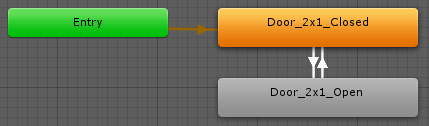
\includegraphics[width=0.5\linewidth]{pics/animation_example.PNG}
 \captionof{figure}[Beispiel für einen \textit{Animator}]{Beispiel für den Zustandsautomaten eines \textit{Animators} für eine Tür.}
	\label{fig:animator_example}
\end{figure}

Animationen an sich haben soweit noch keinen Effekt auf eine laufende Spielszene. Hierzu muss zu dem Spielobjekt, welches animiert werden soll, ein sogenannter \textit{Animator} \cite{Unity_Doc_Animator} als Komponente hinzugefügt werden. Dieser definiert über einen Zustandsautomaten die Übergänge zwischen den einzelnen Animationen sowie die Zeitpunkte, wann diese ausgelöst werden, wie in Abbildung \ref{fig:animator_example} anhand einer Türanimation zu sehen ist. "`Door\_2x1\_Open"' und "`Door\_2x1\_Close"' sind im Beispiel die entsprechenden Einzelanimationen zum Öffnen und Schließen der Tür. Die Übergänge zwischen den einzelnen Zuständen können entweder zeitlich oder durch Setzen entsprechender selbst definierter Variablen ausgelöst werden. Jede Animation wird beim Zustandsübergang zu dieser einmal abgespielt und, sofern dementsprechend definiert, bis zum nächsten Übergang wiederholt.

Für statische Elemente der Benutzeroberfläche wird als Eltern-Spielobjekt zumeist ein \textit{Canvas} \cite{Unity_Doc_Canvas} eingesetzt. Dieser erstreckt sich in der Regel über den gesamten Bildschirm und dient als Anker für alle Kindelemente. So können Objekte für die Benutzeroberfläche zum Beispiel relativ zum \textit{Canvas} in der rechten oberen Ecke platziert werden. Dies gewährleistet, dass die Oberflächenelemente dynamisch mit der Bildschirmgröße skalieren und entsprechend positioniert werden, sodass die Oberfläche unabhängig von der Bildschirmauflösung ist.
\pagebreak

% Levelaufbau
\section{Levelarchitektur und grundlegende Bestandteile}\label{sec:levelArchitecture}
Der erste Schritt zur Realisierung des Spiels besteht darin, die Struktur für das Level an sich umzusetzen. Dazu gehört zuallererst eine entsprechende Architektur im technischen Sinne zu gestalten. Der Aufbau und die Verwaltung der Levelstruktur ist essenziell für alle weiteren Komponenten der Software, da nahezu alle diese mit dem Level interagieren müssen. Das Spiellevel mitsamt aller Bestandteile ist somit der zentrale Punkt, an dem das Spiel abläuft.

Im folgenden Abschnitt \ref{sec:levelStructure} werden deshalb das Design und die Funktionsweise des Levels exakt erläutert. Ebenso wird in Kapitel \ref{sec:levelElements} die konkrete Umsetzung der einzelnen Level-Elemente genauer beleuchtet. Dazu zählt zum einen die spezifische Logik hinter den einzelnen Elementen und zum anderen auch deren grafische Darstellung im Spiel.

\subsection{Der Grundaufbau der Levelstruktur}\label{sec:levelStructure}
Bevor mit dem Entwurf des Levelaufbaus begonnen werden kann, muss zunächst geklärt werden, wie ein Spiellevel insgesamt aussehen soll. Dazu gehört zunächst der geometrische Aufbau des Levels. Hier gilt es, die Designentscheidung zu treffen, ob Gegenstände beziehungsweise Elemente frei platzierbar sein sollen oder ob das Level in einzelne Teile unterteilt werden soll, auf denen sich dann die jeweiligen Elemente befinden. In diesem Anwendungsfall ist der letztere Ansatz die präferierte Lösung.

Konkret soll ein Level aus einem Raster aus quadratischen Teilen bestehen. Dies hat zwar den Nachteil, dass statische Elemente wie Türen und Wände später an dieses Raster gebunden sind, jedoch vereinfacht dies die Lösung einiger Probleme. Erstens ist die Serialisierung von Spielleveln durch diesen Ansatz weniger komplex, da für die einzelnen Levelbestandteile nur die Rasterkoordinaten gespeichert werden müssen (Details siehe Kapitel \ref{sec:structureSerialization}). Zweitens vereinfacht ein teilebasierter Levelaufbau die Navigation auf dem Spielfeld, worauf in Kapitel \ref{sec:pathfindingConcept} noch genauer eingegangen wird. Ein weiterer wichtiger Grund ist, dass so die Levelteile in einem zweidimensionalen Feld organisiert werden können, wie im UML-Diagramm in Abbildung \ref{fig:level_structure} zu sehen ist. Dies ermöglicht eine strukturierte Verwaltung der Levelbestandteile und einen leichteren koordinatenbasierten Zugriff auf die Teile im Level. Eine Unterteilung des Levels in ein quadratisches Raster bedeutet aber ausdrücklich nicht, dass zum Beispiel Gegner, Gegenstände oder der Spieler an dieses Raster gebunden sind. Lediglich statische Level-Elemente sollen daran gebunden sein.

\begin{figure}[h]
 \centering
 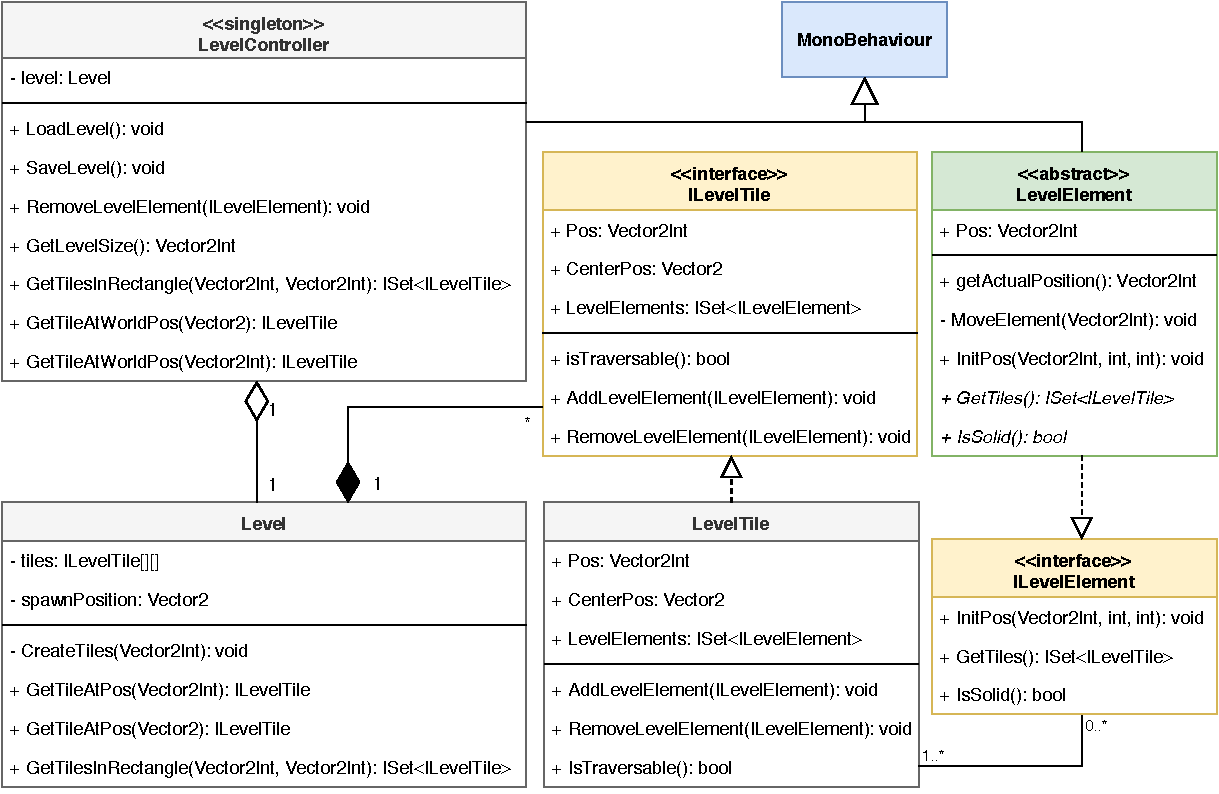
\includegraphics[width=1.0\linewidth]{diagrams/Level_Data_Structure.pdf}
 \captionof{figure}[Datenstruktur des Levels]{UML-Klassendiagramm der grundlegenden Levelstruktur in reduzierter Darstellung.}
	\label{fig:level_structure}
\end{figure}

Neben den einzelnen Levelteilen speichert das Level außerdem auch die Startposition des Spielers und bietet über diverse Methoden Zugriff auf die einzelnen Levelteile über Weltkoordinaten. Um die Level-Datenstruktur vor Manipulationen von außen zu schützen, übernimmt der \texttt{LevelController} die Verwaltung des Levels. Dieser existiert in der Unity-Szene für das eigentliche Spiel als einzelnes Spielobjekt und stellt alle notwendigen Operationen auf dem Level nach außen zur Verfügung. Der Controller hält außerdem eine Referenz auf die Datenstruktur des Levels und ist zuständig für das Speichern und Laden von Leveln. Wie dies konkret funktioniert, wird in Kapitel \ref{sec:designSerialization} im Zuge der Levelserialisierung und Deserialisierung genauer erläutert. Zusammenfassend bildet der \texttt{LevelController} also eine Zwischenschicht zwischen Zugriffen von außen und dem zugrundeliegendem Modell in Form des Levels.

Das Interface \texttt{ILevelTile}, aus dem sich das Level zusammensetzt, und welches die konkrete Klasse \texttt{LevelTile} implementiert, beinhaltet drei Eigenschaften:
\begin{itemize}
	\item \texttt{Pos}: Die linke untere Position des \texttt{ILevelTile} im Level.
	\item \texttt{CenterPos}: Die Koordinaten der Mitte des Teils. Diese Eigenschaft dient vor allem der Bequemlichkeit, um häufige Umrechnungen mit der tatsächlichen Position zu vermeiden.
	\item \texttt{LevelElements}: Alle Level-Elemente, die auf diesem Teil platziert sind.
\end{itemize}

Über die Methoden \texttt{AddLevelElement(...)} und \texttt{RemoveLevelElement(...)} können zur Laufzeit dynamisch Level-Elemente einem Teil zugeordnet und wieder entfernt werden. Die \texttt{Is\-Tra\-ver\-si\-ble()}-Methode dient dazu, zu ermitteln, ob zum Beispiel Gegner über dieses Teil laufen können und wird vor allem innerhalb des Wegfindesystems (siehe Kapitel \ref{sec:pathfindingConcept}) utilisiert. Die Entscheidung, ob ein \texttt{LevelTile} traversierbar ist, wird dabei basierend auf den darauf platzierten Level-Elementen getroffen.

Die \texttt{Level}-Klasse und die zugehörigen \texttt{ILevelTile} bieten soweit eine flexible Grundstruktur für das Level, jedoch fehlt noch eine Integration der tatsächlich in der Unity-Szene enthaltenen und für den Spieler sichtbaren Objekte in die beschriebene Datenstruktur. Diese Rolle übernehmen die bereits vorher erwähnten Level-Elemente. Ein solches Element ist konkret jeder beliebige statische Gegenstand der auf dem Level platziert werden kann, wie zum Beispiel eine Wand. Details zu den einzelnen implementierten Elementen folgen hierzu in Abschnitt \ref{sec:levelElements}. Alle Elemente müssen zumindest das \texttt{ILevelElement}-Interface implementieren. Mit Ausnahme von Böden erben alle anderen direkt von der abstrakten Klasse \texttt{LevelElement}, die bereits generische Logik implementiert. Die \texttt{LevelElement}-Klasse erbt wiederum von \texttt{MonoBehaviour}, wodurch es sich direkt als Komponente zu Spielobjekten in der Szene hinzufügen lässt.

Die \texttt{InitPos(...)}-Methode muss bei jedem Level-Element nach der Erzeugung mit der ge\-wünsch\-ten Position als Eingabe aufgerufen werden und registriert das Element anhand der Position und der Größe in X- und Y-Achsenrichtung bei den Levelteilen, auf denen es sich befindet und setzt die Position des zugehörigen Spielobjekts in der Welt entsprechend. Per Aufruf von \texttt{GetTiles()} lassen sich schließlich alle Levelteile, auf denen sich das Element befindet, zurückgeben. Dabei ist anzumerken, dass ein \texttt{LevelElement} keine direkte Referenz auf diese Levelteile hat, um eine zweiseitige Referenzierung zwischen den Teilen und Elementen zu vermeiden. Stattdessen nutzen die konkreten Implentierungen von \texttt{ILevelElement} die eigene Position und die Hilfsmethoden des \texttt{LevelController}, um auf die zugehörigen Teile zuzugreifen. Da die verschiedenen Levelelemente auch mehrere Teile groß sein und verschiedene Formen haben können, muss die \texttt{GetTiles()}-Methode von einer konkreten Unterklasse ausimplementiert werden, weil so das inhärente Wissen über die Form des Elements zur Ermittlung der zugeordneten Levelteile genutzt werden kann. Über den Aufruf von \texttt{IsSolid()} lässt sich schließlich noch ausgeben, ob ein Level-Element solide, also nicht begehbar ist. Dies wird deshalb über eine Methode anstatt einer einfachen boolschen Variable geregelt, weil sich der Rückgabewert zur Laufzeit ändern kann, wie zum Beispiel bei einer Tür, die verschlossen wird.

Über die Eigenschaft \texttt{Pos} lässt sich bei jedem abstrakten \texttt{LevelElement} außerdem die Position während des Spiels ändern. Die Methode \texttt{MoveElement(...)} bewegt dann automatisch das zugehörige Spielobjekt und aktualisiert die Referenzen der Levelteile auf dieses Level-Element, sodass diese mit der neuen Position übereinstimmen. \texttt{GetActualPosition()} gibt die tatsächlichen Weltkoordinaten des Spielobjekts des Level-Elements zurück.

Mit der beschriebenen Datenstruktur des Levels ist es also zusammenfassend möglich, Spielobjekte für die tatsächlichen Elemente des Levels flexibel auf dessen Raster zu platzieren und zu verschieben. Ebenso lassen sich alle für die Spiellogik relevanten Daten positionsbasiert durch die einzelnen Teile des Levels ermitteln.
 
\subsection{Die Level-Elemente des Spiels}\label{sec:levelElements}
Um ein Level mit sichtbaren Gegenständen populieren zu können, müssen noch die entsprechenden Level-Elemente implementiert werden. Wie die einzelnen Elemente, sowohl aus Sicht der damit verbundenen Logik, als auch in Bezug auf die grafische Darstellung umgesetzt sind, wird in den folgenden Abschnitten genau erläutert.

\begin{figure}[h]
 \centering
 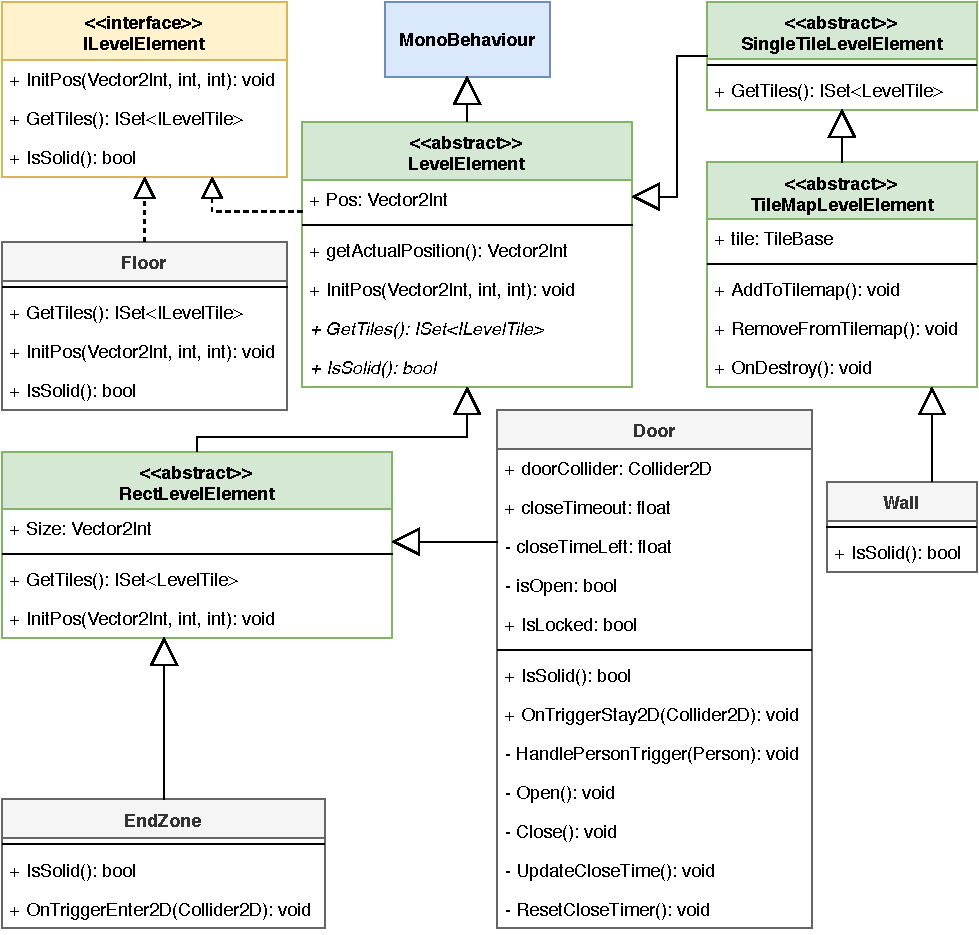
\includegraphics[width=0.86\linewidth]{diagrams/Level_Element_UML.pdf}
 \captionof{figure}[Übersicht über die Level-Elemente des Spiels]{UML-Klassendiagramm aller Level-Elemente des Spiels.}
	\label{fig:level_elements}
\end{figure}

Vor der konkreten Implementierung werden die Level-Elemente zunächst über die abstrakten Klassen \texttt{RectLevelElement} und \texttt{SingleTileLevelElement} weiter in größere rechteckige Elemente, und welche, die nur ein einzelnes Teil umfassen unterteilt, wie anhand des UML-Diagramms in Abbildung \ref{fig:level_elements} zu sehen ist. Beide implementieren die \texttt{GetTiles()}-Methode, da diese für jeweils alle Unterelemente gleich ist. Das \texttt{RectLevelElement} überschreibt zudem \texttt{InitPos(...)}, um bei der Initialisierung die Ausmaße des Elements in der entsprechenden Eigenschaft \texttt{Size} abzuspeichern. Der Nutzen des \texttt{TileMapLevelElement} wird im Folgeabschnitt \ref{sec:wall} am Beispiel der Wände im Level erklärt.

Allgemein wäre eine so feine Unterteilung durch die abstrakten Oberklassen in der aktuellen Form des Spiels noch nicht zwangsläufig notwendig gewesen. Unter dem Gesichtspunkt, dass zu einem späteren Zeitpunkt gegebenenfalls weitere Elemente hinzugefügt werden sollen, ist dies aber so mit einem nur sehr geringen Arbeitsaufwand möglich und daher dennoch sinnvoll.

\subsubsection{Wände}\label{sec:wall}
Wände sind die zentralen Bestandteile zur Aufteilung des Levels und sind genau ein Teil groß. Alle Spielobjekte, die eine Wand sind, besitzen zusätzlich einen quadratischen \textit{Collider2D}, sodass sie nicht durch den Spieler oder Gegner traversierbar sind.

Aus Sicht der Logik stellt dies bereits alles Relevante zu den Wänden dar, jedoch ergibt sich im Bezug auf die Grafik ein Problem. Sind mehrere Wände nebeneinander platziert, sollten sich die Texturen automatisch so anpassen, dass es so scheint als wären sie verbunden, wie in Abbildung exemplarisch \ref{fig:connected_walls} dargestellt ist.

\begin{figure}[h]
 \centering
 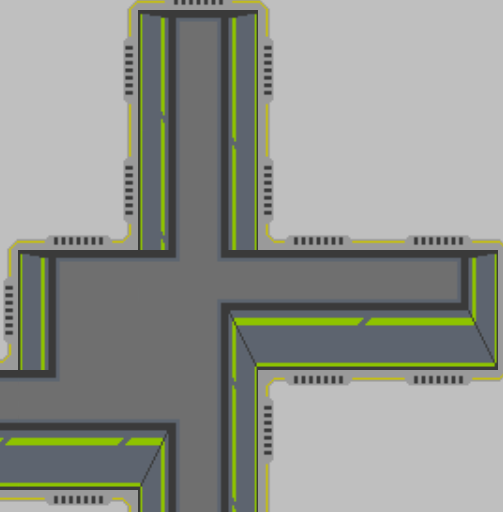
\includegraphics[width=0.3\linewidth]{pics/connected_walls.png}
 \captionof{figure}[Automatische Wandtexturverbindung]{Beispiel aus dem Spiel bei dem sich die Texturen mehrerer Wände automatisch verbinden. Bei den Bodenteilen ist selbiges zu sehen.}
	\label{fig:connected_walls}
\end{figure}

Mit einfachen Texturen auf den einzelnen Wandelementen wäre dies nur mit größerem Programmieraufwand zu lösen. Eine einfachere Lösung bietet hier die Verwendung einer sogenannte \textit{Tilemap} von Unity in Kombination mit \textit{RuleTiles}. Eine \textit{Tilemap} ist vereinfacht dargestellt ein Raster, bei dem jedem Feld des Rasters ein sogenanntes \textit{Tile} zugewiesen werden kann. Dies ist nicht zu verwechseln mit den Teilen in der Levelstruktur, denn die Teile der \textit{Tilemap} definieren lediglich eine grafische Repräsentation. Das \textit{RuleTile} ist dabei eine von Unity zur Verfügung gestellte Spezialform, die es ermöglicht zu definieren, bei welchen Nachbarschaftsbeziehungen welche Textur für das Teil geladen werden soll. Das heißt, es lässt sich beispielsweise für die Wände definieren, welches Bild für diese Wand angezeigt wird, wenn rechts davon ebenso eine Wand platziert ist. Dies ermöglicht, das vorher beschriebene Problem mit nur geringem Aufwand zu Lösen.

Konkret wird hierzu eine \textit{Tilemap} für Wände angelegt, die sich in der Rastergröße mit der des Levels überlagert, sodass die Teile über der tatsächlichen Position des Levels angezeigt werden. Für solche \textit{Tilemap}-basierte Level-Elemente wird zusätzlich die abstrakte Oberklasse \texttt{TileMapLevelElement} angelegt, von der die Wand erbt. Diese hält eine Referenz auf die Vorlage für das \textit{Tile} und besitzt die Funktionalität, in der \textit{Tilemap} das \textit{Tile} an der entsprechenden Position auf die Vorlage (hier die Wand) zu setzten, beziehungsweise diese wieder zu entfernen. Bei Zerstörung des Spielobjekts der Wand wird das entsprechende \textit{Tile} auf der \textit{Tilemap} automatisch wieder entfernt.

Die Wand ist somit aufgeteilt in das Spielobjekt, welches für die eigentliche Logik verantwortlich ist, sowie die grafische Repräsentation auf der \textit{Tilemap}.

\subsubsection{Böden}\label{sec:floor}
Böden stellen unter den Level-Elementen eine Ausnahme dar, weil sie als einzige nicht von \texttt{LevelElement} erben sondern direkt das \texttt{ILevelElement}-Interface implementieren. Sie sind ebenso wie Wände ein Teil groß und verwenden zur Anzeige auch eine eigene \textit{Tilemap}, sodass die Texturen benachbarter Böden sich verbinden können. Auf den ersten Blick wäre es daher logisch, wenn die Klasse \texttt{Floor} von \texttt{TileMapLevelElement} erben würde. Tatsächlich wäre dies die aus softwarearchitektonischer Sicht gesehen bessere Lösung, da die \texttt{Tilemap}-bezogene Logik komplett wiederverwendet werden könnte.

Der Grund warum sich dagegen entschieden wurde ist, dass Böden an sich keine Logik im Spiel besitzen und der rein dekorativen, grafischen Anzeige dienen. Alle \texttt{LevelElemente} sind aber aufgrund der \textit{MonoBehaviour}-Oberklasse an ein Spielobjekt gebunden. Das bedeutet, dass für jeden Boden ein Spielobjekt angelegt werden würde, was de-facto in der Szene ohne Nutzen ist, weil keine Logik an ein Bodenteil gebunden ist. Es würde also unnötigerweise Arbeitsspeicher und Rechenzeit für die Spielobjekte der Böden verbraucht werden. Deshalb implementieren diese nur das entsprechende Interface für Level-Elemente und existieren so nur innerhalb der Datenstruktur des Levels und als grafisches \textit{Tile} in der entsprechenden \textit{Tilemap}. Das setzen des \textit{Tiles} erfolgt dabei unmittelbar nach der Erzeugung eines Boden-Objekts.

\subsubsection{Türen}\label{sec:door}
Die Türen sind in Bezug auf die damit verbundene Spiellogik die komplexesten Level-Elemente, was in Abbildung \ref{fig:level_elements} bereits zu erkennen ist. Es handelt sich dabei um ein \texttt{RectLevelElement}, da diese je nach Rotation zwei Teile breit sind. Der Spielausschnitt in Abbildung \ref{fig:door_opening} zeigt, wie sich die Tür automatisch bei Annäherung eines Spielers oder Gegners öffnen soll.

\begin{figure}[h]
 \centering
 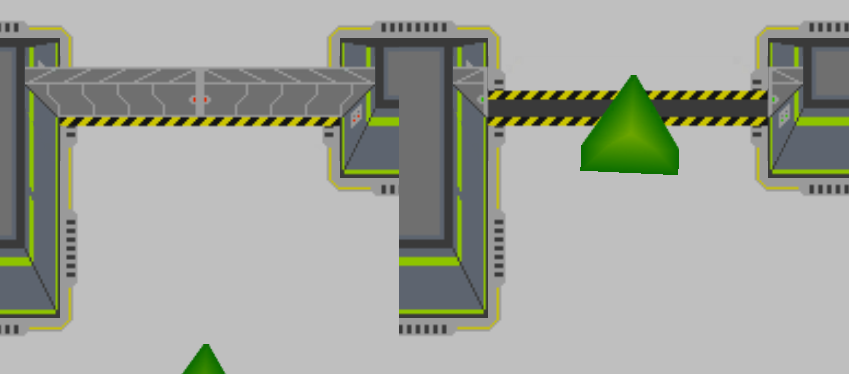
\includegraphics[width=0.6\linewidth]{pics/traversing_door.png}
 \captionof{figure}[Automatischen öffnen einer Tür]{Automatisches Öfnen einer Tür bei Annäherung einer Person.}
	\label{fig:door_opening}
\end{figure}

Um dieses Verhalten zu realisieren, werden zwei verschiedene rechteckige \textit{Collider2D} eingesetzt. Einer ist deutlich größer als die Tür und ist als sogenannter \textit{Trigger} gesetzt. Das bedeutet, dass bei Kontakt mit einem anderen physikalischen Objekt von der Physik-Engine entsprechende Methoden, wie hier \texttt{OnTriggerStay2D(...)}, aufgerufen werden, aber keine tatsächlichen Kollisionen simuliert werden. Der Spieler prallt also beispielsweise nicht von diesem \textit{Collider2D} ab. Befindet sich eine Person in diesem Bereich, wird die Tür geöffnet und die Zeit bis die Tür wieder geschlossen wird zurückgesetzt. Befindet sich keine Person mehr in diesem \textit{Trigger}-\textit{Collider2D}, schließt sich die Tür nach Ablauf des \texttt{closeTimeout} wieder.

Die Tür hält zudem eine Referenz auf einen weiteren \textit{Collider2D}, der so groß wie die Tür an sich ist. Im Gegensatz zu ersterem verursacht dieser Kollisionen, sodass bei geschlossener Tür zum Beispiel Schüsse daran aufprallen. Wird die Tür geöffnet, wird dieser dann vorübergehend deaktiviert. Die Eigenschaft \texttt{IsLocked} ermöglicht außerdem die Tür zu versperren, wodurch sie sich nicht mehr automatisch bei Annäherung einer Person öffnet. Diese Funktionalität wird zwar im aktuellen Stand nicht verwendet, eröffnet aber Möglichkeiten für zukünftige Erweiterungen.

Für das Öffnen und Schließen der Tür existieren zudem entsprechende Animationen. Die Zustandsübergänge des zugehörigen \textit{Animators} wurden bereits beispielhaft in Abbildung \ref{fig:animator_example} dargestellt.

\subsubsection{Endzone}\label{sec:endZone}
In diesem Spiel soll es dem Spieler nicht nur möglich sein durch Eliminierung aller Gegner zu gewinnen. Stattdessen soll es ebenso ermöglicht werden den Sieg durch Erreichen einer Level-Endzone zu erringen, indem die Gegner geschickt aus­ma­nö­v­rie­rt werden. Dadurch soll auch leises Vorgehen seitens des Spielers belohnt werden.

Diese Endzone muss allerdings noch in das Spiel integriert werden. Hierzu wird ein weiteres \texttt{RectLevelElement} namens \texttt{EndZone} erstellt. Das zugehörige Spielobjekt enthält neben der Textur, ähnlich wie die Tür, einen als \textit{Trigger} dienenden \textit{Collider2D}. Sobald ein physikalisches Objekt mit diesem eine Kollision auslöst, wird die \texttt{OnTriggerEnter2D(...)}-Methode aufgerufen. Handelt es sich bei dem kollidierenden Objekt um den Spieler, gilt das Spiel als gewonnen und das Menü zum Spielende öffnet sich. Von dort aus kann der Nutzer das Level entweder neu starten, oder in das Hauptmenü zurückkehren.
\pagebreak

% Charaktere und Waffen
\section{Charaktere und Items im Spiel}\label{sec:charactersAndItems}
Neben den statischen Level-Elementen benötigt es noch Charaktere in Form von Gegnern und dem Spieler selbst, die sich darauf fortbewegen können. Wie diese grundlegend aufgebaut sind, wird in Abschnitt \ref{sec:charactersBasic} dargestellt. Dabei wird insbesondere auch auf den Spieler und die zugehörige Benutzeroberfläche für den Endnutzer eingegangen. Da die konkrete Umsetzung der Gegner eine umfangreiche Thematik ist, wird dies separat in Kapitel \ref{sec:enemiesAndAI} behandelt.

Im Folgenden wird außerdem erläutert, wie interagierbare Gegenstände, also vornehmlich Waffen, in das Spiel integriert sind.

\subsection{Grundaufbau von Charakteren im Spiel}\label{sec:charactersBasic}
Auch wenn der Spieler und die Gegner sich in ihrer Funktionsweise stark unterscheiden, besitzen beide auch einige gemeinsame Eigenschaften. Aus diesem Grund erben sowohl der Spieler, als auch die Gegner von \texttt{Person} (siehe Abbildung \ref{fig:person_structure}). Jeder Charakter besitzt somit eine Anzahl an Lebenspunkten und Parameter zur Einstellung des Laufverhaltens, also zum Beispiel die Maximalgeschwindigkeit oder Beschleunigung der Person. Durch Implementierung des \texttt{IDamageable}-Interfaces ist es möglich jeder Person beispielsweise durch ein Projektil Schaden zufügen zu können. Die \texttt{Damage(...)}-Methode erhält dabei als Eingabeparameter die Anzahl an Schaden in Form von Lebenspunkten und eine Referenz auf das schadensverursachende Spielobjekt. Letzteres ist nötig, um zu erkennen, ob zum Beispiel bei Gegnern der Schaden von einem anderen Gegner verursacht wurde, und somit ignoriert werden soll.

\begin{figure}[h]
 \centering
 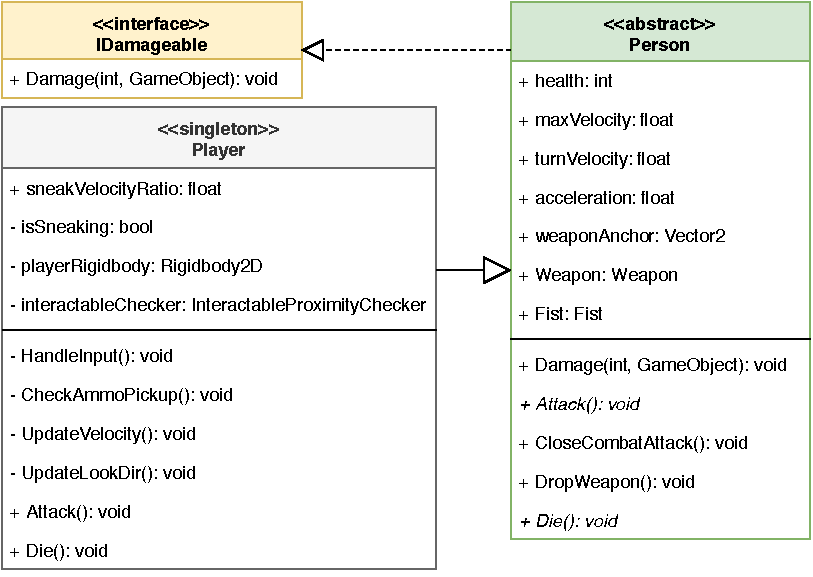
\includegraphics[width=0.8\linewidth]{diagrams/characters_reduced_UML.pdf}
 \captionof{figure}[Grundaufbau von Charakteren]{Vereinfachtes UML-Klassendiagramm der \texttt{Person}-Klasse und des Spielers}.
	\label{fig:person_structure}
\end{figure}

In der Klasse \texttt{Person} existiert zusätzlich je eine Referenz auf eine Waffe und eine Faust, die für Attacken genutzt werden können. Die Faust dient dabei zur Verwendung in Nahkampfangriffen über Aufruf der Methode \texttt{CloseCombatAttack()}, für den Fall, dass die Person aktuell keine andere Waffe besitzt. Sowohl die Klasse \texttt{Fist}, als auch \texttt{Weapon}, werden später in Abschnitt \ref{sec:weaponImplementation} genauer erklärt. Der \texttt{weaponAnchor} gibt noch an, in welchem räumlichen Versatz eine getragene Waffe zum Spielobjekt der Person platziert werden soll. Über die \texttt{DropWeapon()}-Methode kann ein Charakter dazu veranlasst werden seine aktuelle Waffe auf den Boden fallen zu lassen.

Alle Unterklassen von \texttt{Person} müssen außerdem die Angriffsmethode und die Methode \texttt{Die()} implementieren. Letztere wird aufgerufen, sobald die Anzahl der Lebenspunkte unter den Wert eins fällt.

Ähnlich wie für das Level, existiert hier ein sogenannter \texttt{PersonController}, der die Personen auf dem Level verwaltet. Er ermöglicht Zugriff auf die Charaktere im Level und ist bei Levelstart für deren Instanziierung zuständig. Dies geschieht unter Verwendung entsprechender Fabrikmethoden, die über \textit{Prefabs} Spielobjekte in der Szene erzeugen und mit den korrekten Parametern, wie unter anderem deren Position aufsetzen.

\subsubsection{Umsetzung des Spielers und dessen Steuerung}\label{sec:player}
Der Spieler, der schließlich vom Nutzer gesteuert wird, ist eine konkrete Implementierung der \texttt{Person}-Klasse und kann maximal einmal pro Szene in Unity existieren, wie in Abbildung \ref{fig:person_structure} zu sehen ist.

Bei jedem Aufruf der \texttt{Update()}-Methode der Unity-Engine werden über die \texttt{HandleInput()}-Methode die Nutzereingaben zur Steuerung des Spielers verarbeitet. Über die Tasten "`W"', "`A"', "`S"' und "`D"' oder die Pfeiltasten lässt sich der Spieler bewegen. Dabei wird der \textit{Rigidbody2D} des Spielers je nach den gedrückten Tasten in die entsprechende Richtung beschleunigt, bis die Maximalgeschwindigkeit erreicht ist. Der Spieler kann dabei zusätzlich bei gehaltener "`Shift"'-Taste schleichen. Dabei bewegt er sich zwar um den Faktor der \texttt{sneakVelocityRatio} langsamer, erzeugt beim Laufen allerdings keine Geräusche mehr, wodurch Gegner, wie in Kapitel \ref{sec:gegnerreaktionaufaudio} genauer beschrieben wird, den Spieler nicht mehr hören können. Zum Zielen dreht sich der Spieler durch Aufruf der \texttt{UpdateLookDir()}-Methode automatisch in die aktuelle Richtung des Mauszeigers.

Die \texttt{Player}-Klasse hält zudem eine Referenz auf einen \texttt{InteractableProximityChecker}. Dies ist eine Hilfsklasse, die dem Spielobjekt des Spielers als Komponente angefügt ist. Diese prüft zyklisch, welche interagierbaren Gegenstände im unmittelbaren Umkreis sind und hebt, sofern vorhanden, den nächsten Gegenstand farblich hervor. Über "`E"' kann der Spieler mit dem nächsten Gegenstand interagieren, also zum Beispiel eine Waffe aufheben. Mit "`Q"' kann eine Waffe zudem wieder fallen gelassen werden. Der \texttt{interactableChecker} wird außerdem verwendet, um automatisch Waffen aufzuheben, wenn sie vom gleichen Typ der aktuellen Waffe sind, um dann deren Munition zur aktuellen hinzuzufügen.

Bei Eliminierung des Spielers wird das aktuelle Level schließlich beendet und der Nutzer kann das Level neu starten, oder ins Hauptmenü zurückkehren.

\subsubsection{Die Benutzeroberfläche des Spielers}\label{sec:uiPlayer}
Um den Spieler die nötigen Informationen zur aktuellen Spielsituation zu vermitteln, wurde eine entsprechende Nutzeroberfläche eingebaut. Hierzu wird in der linken unteren Ecke der Szene die aktuelle Munitionsmenge angezeigt und rechts die Lebenspunkte des Spielers. Da das Spiel auch gewonnen werden kann, indem alle Gegner eliminiert werden, wird zudem in der linken oberen Ecke der Benutzeroberfläche die Anzahl verbleibender Gegner angezeigt, um so die Suche zu erleichtern.

\begin{figure}[h]
 \centering
 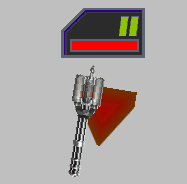
\includegraphics[width=0.2\linewidth]{pics/enemy_hud.PNG}
 \captionof{figure}[Informationsanzeige eines Gegners]{Informationsanzeige eines Gegners mit Lebens- und Aufmerksamkeitsbalken.}
	\label{fig:enemy_hud}
\end{figure}

Der Spieler benötigt zudem Informationen zum Status der einzelnen Gegner. Zu diesem Zwecke befindet sich oberhalb eines jeden Gegners eine entsprechende Anzeige, wie in Abbildung \ref{fig:enemy_hud} zu sehen. Diese zeigt zum einen, ähnlich wie beim Spieler, in Form von grünen Balken die aktuellen Lebenspunkte an. Zum anderen wird im unteren Balken die Spieleraufmerksamkeit des Gegners angezeigt, die angibt, inwieweit die Position des Spielers dem Gegner bekannt ist. Wurde der Spieler entdeckt, wird der Balken rot. Das darunterliegende Aufmerksamkeitssystem der Gegner wird in Kapitel \ref{sec:enemyImplementationAwareness} noch genau behandelt.

\subsection{Interaktive Gegenstände im Spiel}
\label{sec:weapon}

Neben den Level-Elementen und Charakteren spielen auch interaktive Gegenstände (engl. \textit{items}) eine wichtige Rolle. Diese beschränken sich zunächst auf Waffen, aber es wären auch weitere Gegenstände, beispielsweise Munition für die Waffen oder Gegenstände für die Wiederherstellung von Lebenspunkten denkbar.

\subsubsection{Design der Waffen}
\label{sec:weaponDesign}

Die Waffen im Spiel lassen sich in Nahkampf- und Fernkampfwaffen einteilen. Zu den Nahkampfwaffen gehören der Schlagstock sowie die Faust, welche als Unterobjekt jedes Charakters mitinstanziiert wird und zu den Fernkampfwaffen zählen die Pistole, das Maschinengewehr und die Schrotflinte.

Für alle Waffen außer der Faust, die aufgrund der Darstellung der Charaktere als farbige Pfeile unsichtbar ist, gibt es zwei Ansichten: Eine Ansicht von der Seite für im Level abgelegte Gegenstände, und eine von oben, für Gegenstände, die von einem Charakter getragen werden. Für jede dieser Waffen wurde für jede Ansicht ein Bild entweder selbst erstellt oder aus dem Internet ausgewählt und abgeändert (siehe \cite{Sprite_Machinegun} \cite{Sprite_Shotgun} \cite{Sprite_Bat}).

Damit Charaktere am anderen Ende des Levels nicht von Munition getroffen werden können, haben die Patronen eine relativ kurze Lebensdauer, die für jede Munitionssorte separat definiert wird.

\subsubsection{Implementierung der Waffen}
\label{sec:weaponImplementation}

Das gemeinsame Verhalten der Waffen ist in der abstrakten \texttt{Weapon}-Klasse definiert, welche die Interfaces \texttt{Item} und \texttt{IInteractable} implementiert. Von der \texttt{Weapon}-Klasse erben, wie in Abbildung \ref{fig:weaponStructure} gezeigt, wiederum die ebenfalls abstrakten Klassen \texttt{MeleeWeapon} für Nahkampfwaffen und \texttt{FireArm} für Fernkampfwaffen.

Jedem Waffen-\textit{Prefab} ist ein Projektil-\textit{Prefab} zugeordnet, welches in der \texttt{Fire()}-Methode der Waffe instanziiert wird. Dabei wird das Spielobjekt des Charakters, an dem die Waffe hängt, als \texttt{origin} des Projektils übergeben. Trifft der \textit{Collider} des Projektils auf den \textit{Collider} eines Spielcharakters, kann überprüft werden, ob der getroffene Charakter mit dem Ursprung des Projektils identisch ist. Ist dies nicht der Fall, wird die \texttt{Damage(...)} Methode der Person aufgerufen.

\begin{figure}[h]
 \centering
 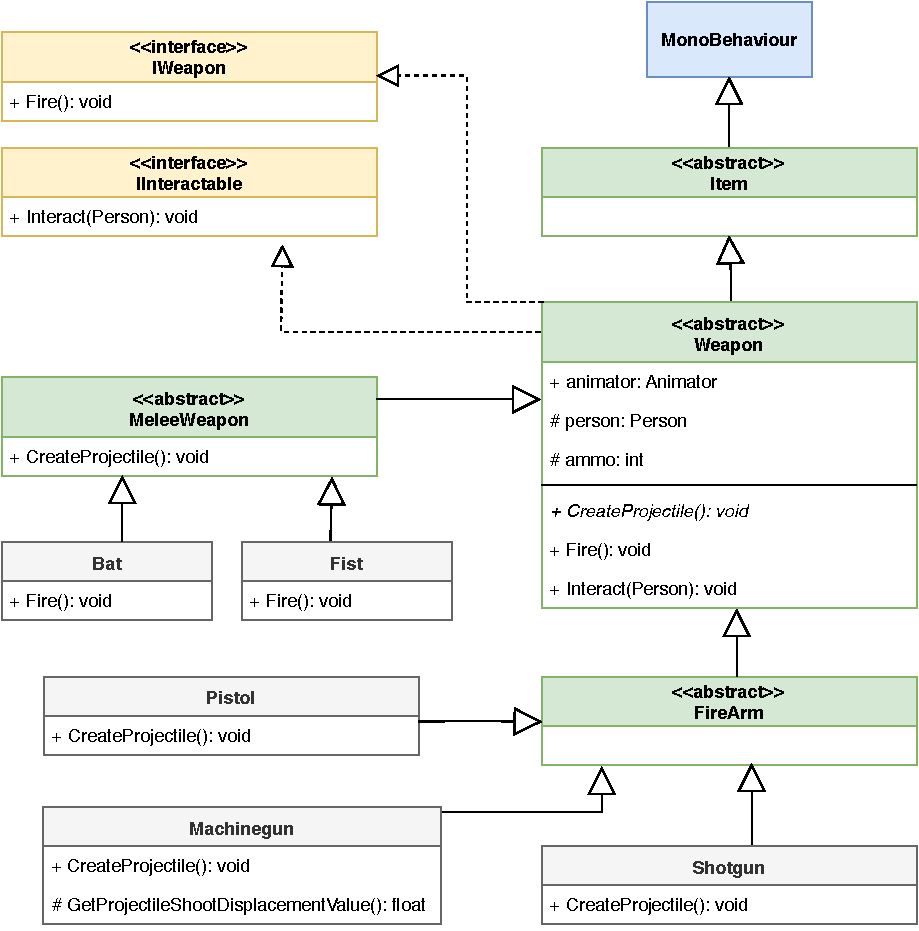
\includegraphics[width=0.835\linewidth]{diagrams/Weapon_Structure_reduced.pdf}
 \captionof{figure}[Datenstruktur der Waffen]{UML-Klassendiagramm der Waffen in reduzierter Darstellung}
	\label{fig:weaponStructure}
\end{figure}

Damit beim Aufnehmen und Ablegen von Waffen das \textit{Sprite} geändert wird, hat jeder Waffentyp außerdem einen entsprechenden \textit{Animator} (siehe Kapitel \ref{sec:unityGrafics}), durch den bei einer Änderung an seiner \texttt{onFloor} Variable eine Animation ausgeführt wird.

\pagebreak

% Gegner und KI
\section{Design und Implementierung der Gegner und ihrer KI}\label{sec:enemiesAndAI}

Für die Entwicklung eines \textit{Schießspiels} (engl. \textit{Shooter}) ist neben der Spielersteuerung und der Waffen auch ein ausgereiftes Konzept für die Gegner unerlässlich. Damit das Spiel Spaß machen kann, müssen diese einerseits den Spieler fordern, dürfen aber andererseits nicht zu schwer zu besiegen sein.

Die Grundidee der Gegner sowie das Konzept für deren \textit{KI} wird in Abschnitt \ref{sec:enemyDesign} beschrieben. In Abschnitt \ref{sec:enemyImplementation} wird auf die Umsetzung der Idee in \textit{Unity} eingegangen. Schließlich wird in \ref{sec:pathfinding} auf die Implementierung des vom Gegner verwendeteten Wegfindungssystems eingegangen.

\subsection{Design der Gegner}
\label{sec:enemyDesign}

Das Design der Gegner ist für das Spiel von zentraler Bedeutung. Dabei wird Wert darauf gelegt, dass das Spiel nicht nur als \textit{Schießspiel}, sondern auch als \textit{Schleichspiel} (engl. \textit{Stealth game}) gespielt werden kann.

Im Folgenden werden das Verhalten der Gegner sowie Gegnervarianten beschrieben.

\subsubsection{Patrouillieren und Angriffsverhalten der Gegner}
\label{sec:enemyDesignAttack}

Die Gegner suchen bei Spielbeginn nicht aktiv nach dem Spieler, sondern haben ein Route, die sie zyklisch ablaufen. Diese Patrouille wird abgebrochen, sobald der Spieler entdeckt wird, was entweder deshalb passiert, weil der Spieler sich im Sichtfeld des Gegners befindet oder weil der Gegner diesen "hört" und sich zu ihm umdreht. Dabei bleibt der Gegner kurz stehen, bevor er zum Angriff übergeht. Dadurch ist der Übergang von Patrouille zu Angriff gut erkennbar und der Spieler hat mehr Zeit, auf den neuen Umstand zu reagieren, bevor er verfolgt wird.

Die Distanz, auf die der Gegner dem Spieler folgt, hängt mitunter von seiner Waffe ab: Hat er keine Waffe oder eine Nahkampfwaffe, versucht er, dem Spieler möglichst nahe zu kommen, um diese einsetzen zu können. Ein Gegner mit Fernkampfwaffe hat dagegen einen bevorzugten Abstand für den Angriff und verfolgt den Spieler nur, solange der Abstand zu diesem größer ist. Geht ihm die Munition aus, so legt er seine Waffe ab und geht zu einem Nahkampfangriff ohne Waffe über. 

Kommt der Gegner beim Verfolgen des Spielers in die Nähe eines anderen Gegners, schließt sich dieser der Verfolgung an, auch, wenn er den Spieler selbst nicht wahrgenommen hatte.

Verschwindet der Spieler aus dem Sichtfeld eines Gegners, so gibt dieser nach kurzer Zeit die Verfolgung auf und kehrt zu seiner Patroullenroute zurück.

\subsubsection{Gegnertypen}
\label{sec:enemyDesignTypes}

Um die Kämpfe abwechslungsreich zu gestalten, werden drei Gegnertypen entworfen, die unterschiedlich auf den Spieler reagieren und verschiedene Merkmale besitzen.

Der erste Gegnertyp, im folgenden als "leichter Gegner“ bezeichnet, wird als Nahkampfgegner konzipiert, der den Spieler erreichen muss, damit er Schaden anrichten kann. Dadurch hat der Spieler etwas länger Zeit, um zu reagieren, nachdem er entdeckt wurde. Damit er aber nicht zu leicht zu besiegen ist, ist der leichte Gegner beim Angriff etwas schneller als andere Gegner.

Der zweite Gegnertyp, der 
„mittelschwerer Gegner“ oder „Standardgegner“ genannt wird, ist dazu in der Lage, mit Fernkampfwaffen umzugehen und hat ein größeres Sichtfeld als der leichte Gegner, wodurch er eine größere Gefahr für den Spieler darstellt, da es schwerer ist, sich anzuschleichen.

Der dritte und letzte Gegnertyp ist am schwierigsten zu besiegen. Das wird einerseits durch bessere Werte bei den Charaktereigenschaften gewährleistet. Beispielsweise hat der „schwere Gegner“ ein größeres Sichtfeld, kann aus einer größeren Entfernung schießen und muss häufiger getroffen werden, bevor er stirbt. Andererseits hat der schwere Gegner zusätzliche Fähigkeiten, die ein intelligenteres Verhalten ermöglichen.

Zuallererst verfügt der schwere Gegner über eine höhere Zielsicherheit. Während die anderen Gegnertypen bei Verfolgung und Fernkampfangriffen auf den aktuellen Standort des Spielers zielen, ist der schwere Gegner dazu in der Lage, vorauszuberechnen, wohin sich der Spieler bewegt. Dadurch ist es für diesen schwieriger, Schüssen auszuweichen und den Gegner abzuhängen.

Das Entkommen wird durch eine hartnäckigere Verfolgung zusätzlich erschwert. Wenn der Spieler aus dem Sichtfeld eines Gegners verschwindet, wird er im Falle eines leichten oder mittelschweren Gegner nur zu dem Punkt verfolgt, an dem dieser ihn zuletzt gesehen hat. Der schwere Gegner ist für kurze Zeit dazu in der Lage, den Spieler auch dann weiter zu verfolgen, wenn sich dieser nicht im Sichtfeld befindet. Darauf wird in Kapitel \ref{sec:pathfindingIntegration} näher eingegangen.

Außerdem ist der schwere Gegner dazu in der Lage, andere Gegner des gleichen Typs auf die aktuelle Position des Spielers aufmerksam zu machen. Damit haben diese eine Art Schwarmintelligenz, die sich jedoch nur auf die Schwierigkeit des Spiels auswirkt, wenn mehrere Gegner von diesem Typ im Spiel sind.

\subsection{Implementierung des Gegnerverhaltens}
\label{sec:enemyImplementation}

Da das Gegnerverhalten relativ komplex ist, macht es einen großen Teil des Projekts aus. Deshalb wird in diesem Kapitel auf die wichtigsten Aspekte näher eingegangen.

Der Abschnitt \ref{sec:enemyImplementationTypes} behandelt dabei das Grundkonzept sowie die Struktur der Implementierung. Im Abschnitt \ref{sec:enemyImplementationFOV} wird auf das Sichtfeld der Gegner eingegangen, da dieses für die Weiterentwicklung des Spiels eine wichtige Rolle spielt (siehe \ref{sec:interfaceSerialization}). Der Abschnitt \ref{sec:enemyImplementationAwareness} befasst sich mit der Wahrnehmung der Gegner, wobei die Wahrnehmung von Geräuschen aufgrund der Komplexität des Audiosystems in Kapitel \ref{audio} separat behandelt wird.

\subsubsection{Implementierung der Gegnertypen}
\label{sec:enemyImplementationTypes}

Für die drei in \ref{sec:enemyDesignTypes} beschriebenen Gegnertypen gibt es jeweils ein \textit{Prefab} mit einem \textit{MonoBehaviour} für das Verhalten sowie einer eigenen Grafik zur Unterscheidung der Gegnertypen im Spiel.

In einer frühen Phase der Entwicklung wird das Verhalten als klassische Vererbungshierarchie umgesetzt, es gibt also die abstrakte Klasse \texttt{Enemy}, welche von der \texttt{Person} Klasse erbt und darunter die Klassen \texttt{EasyEnemy}, \texttt{BasicEnemy} und \texttt{HardEnemy}.

Das Verhalten, das alle Gegner gemeinsam haben, wird dabei in der abstrakten Klasse implementiert. Dazu gehört insbesondere xdie Patrouille, bei der eine Liste an Koordinaten zyklisch abgelaufen wird. Auch parametrisierbare Unterscheidungsmerkmale wie die Anzahl an Leben, die Größe des Sichtfeldes und die Geschwindigkeiten für Patrouille und Angriff befinden sich hier. Diese Variablen werden als \texttt{public} definiert, damit die Werte einfach direkt am \textit{Prefab} eingestellt werden können.

Die typspezifischen Fähigkeiten der Gegner werden dagegen in den Unterklassen implementiert. Das bedeutet, dass das Nahkampfverhalten in der \texttt{EasyEnemy}-Klasse definiert ist, das einfache Fernkampfverhalten in der \texttt{BasicEnemy}-Klasse und das intelligente Verhalten in der \texttt{HardEnemy}-Klasse.

Eine spätere Designanpassung, welche sich auf das Verhalten der Fernkampfgegner bei Fehlender Munition betrifft, ermöglicht eine Konsolidierung, da das Nahkampfverhalten nun für alle Gegnertypen benötigt wird und das intelligente Fernkampfverhalten des schweren Gegners nun als Erweiterung des Standardfernkampfverhaltens verstanden wird.

\begin{figure}[h]
 \centering
 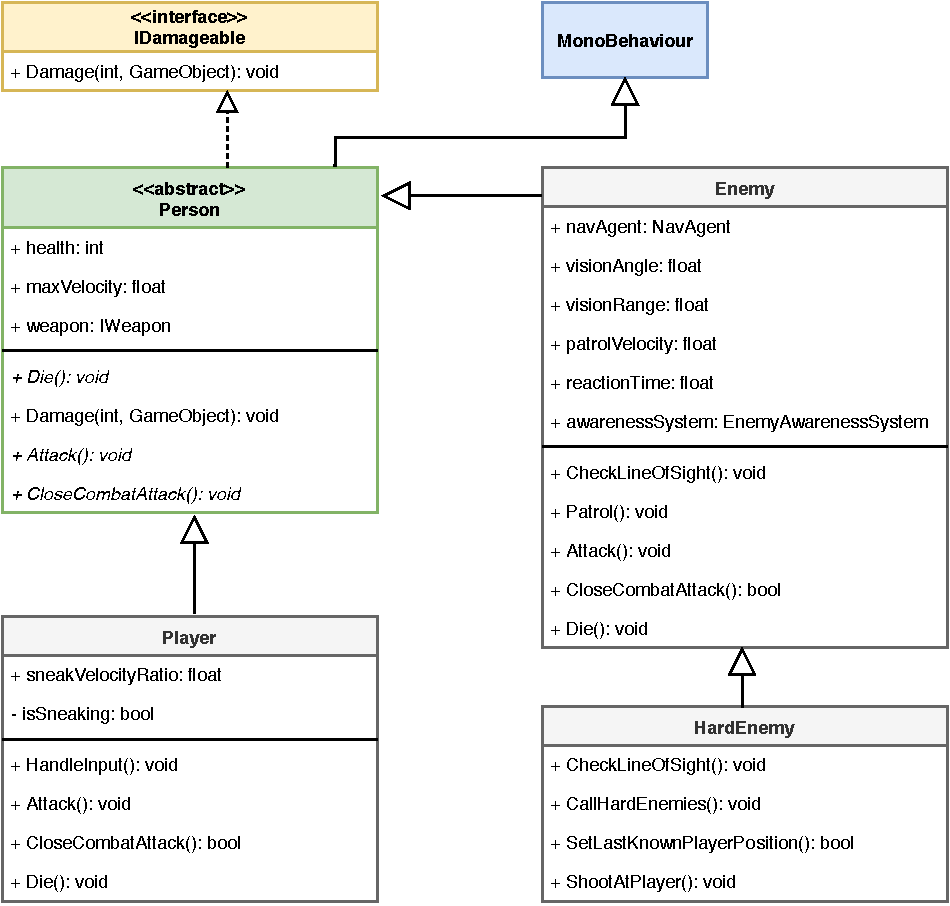
\includegraphics[width=0.835\linewidth]{diagrams/Person_Structure_reduced.pdf}
 \captionof{figure}[Datenstruktur der Charaktere]{UML-Klassendiagramm der Spielcharaktere in reduzierter Darstellung}
	\label{fig:charactersStructure}
\end{figure}


Die \texttt{Enemy}-Klasse ist deshalb nicht mehr abstrakt, sondern kann direkt an die \textit{Prefabs} der leichten und mittelschweren Gegner angehängt werden. Nur der schwere Gegner hat, wie in Abbildung \ref{fig:charactersStructure} zu sehen ist, noch eine eigene Unterklasse.

Diese Struktur lässt sich natürlich noch weiter verbessern. Es wäre beispielsweise möglich, die leichten und mittelschweren Gegner als eingeschränkte Varianten des schweren Gegners zu verstehen und auf dieser Grundlage alle Gegnertypen in der \texttt{Enemy}-Klasse zusammenzufassen. Die Unterschiede würden dann durch öffentliche Variablen festgelegt werden, d.h. die Gegnertypen würden sich nur noch an den Einstellungen am \textit{Prefab} unterscheiden.

Da die \texttt{Enemy}-Klasse ohnehin schon sehr umfangreich ist, wäre es eine sauberere Alternative, das Decorator-Entwurfsmuster zu verwenden. Wie in Kapitel \ref{sec:pathfindingIntegration} beschrieben, wird dieses für die Spielerverfolgung bereits eingesetzt. Die Schwarmintelligenz der schweren Gegner sowie die beiden Fernkampfvarianten könnten genauso umgesetzt werden. Das hätte den Vorteil, dass ohne Probleme neue Gegnerklassen oder neue Fähigkeiten der Gegner eingeführt werden können, ohne, dass an der bestehenden Klassenhierarchie etwas geändert werden muss.

\subsubsection{Das Sichtfeld der Gegner}
\label{sec:enemyImplementationFOV}

Das Sichtfeld des Gegners wird durch einen Blickwinkel und eine Reichweite definiert. Damit diese direkt am Prefab geändert werden können, sind diese Variablen \texttt{public}. Sie werden in der Methode \texttt{CheckLineOfSight()} benötigt, welche von der \texttt{Update()} Methode aufgerufen wird, um zu prüfen, ob sich der Spieler im Sichtfeld befindet.

Um die korrekte Implementierung des Sichtfeldes zu überprüfen, wird eine Visualisierung des Sichtfeldes eingebaut. Die einfachste Möglichkeit dafür ist die Verwendung der \textit{Gizmo}-Klasse \cite{Unity_Doc_Gizmo}, wie sie in Abbildung \ref{fig:fov1} zu sehen ist. Zur Fehlersuche ist diese Darstellung mithilfe eines Kreises für die Sichtweite und zweier Linien für den Blickwinkel zunächst ausreichend.

\begin{figure}[h]
 \centering
 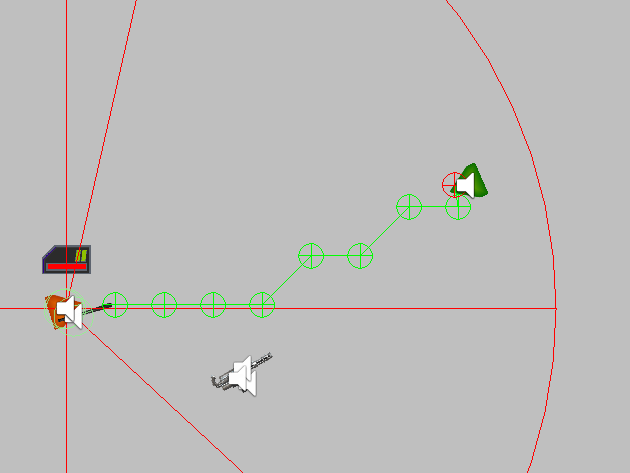
\includegraphics[width=0.835\linewidth]{pics/field-of-view_gizmo.png}
 \captionof{figure}[Visualisierung des Sichtfelds (Version 1)]{Visualisierung des Sichtfelds mit \textit{Gizmo}. Neben dem Sichtfeld werden hier auch die \textit{Gizmos} für Audioquellen und Pfadfindung angezeigt.}
	\label{fig:fov1}
\end{figure}

Mithilfe des \textit{Gizmos} kann im Unity Editor die Reaktion des Gegners auf ein Betreten des Sichtfeldes überprüft werden. Allerdings reagiert das \textit{Gizmo} nicht auf Objekte im Spielfeld, weshalb es so wirkt, als könnte der Gegner durch Wände hindurchsehen, was jedoch nicht der Fall ist. Hinzu kommt, dass Unity automatisch einen Fadenkreuz mitzeichnet, was die Übersichtlichkeit der Visualisierung beeinträchtigt.

Um dieses Problem zu lösen, gibt es mehrere Möglichkeiten. Eine davon wäre, das Sichtfeld mithilfe eines Lichtkegels mit entsprechendem Winkel und entsprechender Reichweite darzustellen. Das hätte den Vorteil, dass die Darstellung des Sichtfeldes automatisch auf Hindernisse im Spiel reagieren würde, aber den entscheidenden Nachteil, dass ein rechenintensives Lichtsystem eingeführt werden müsste, damit die Lichtkegel sichtbar werden \cite{Unity_Doc_Lighting}.

Die Alternative ist das Zeichnen einer Linie für den Umriss des Sichtfeldes. Dafür wird für jeden Winkel des Sichtfeldes mithilfe der Unity-Klasse \texttt{RayCast} überprüft, ob sich ein Hindernis im Sichtfeld befindet und welchen Abstand dieses zum Gegner hat \cite{Unity_Doc_RayCast}.

Da das Sichtfeld bei dieser Variante ohnehin als Linie dargestellt wird, bietet sich auch die Verwendung des \textit{LineRenderers} an \cite{Unity_Doc_LineRenderer}, wie sie in Abbildung \ref{fig:fov2} zu sehen ist. Das hat den Vorteil, dass das Sichtfeld ohne Zusatzaufwand auch im Spiel angezeigt werden kann und nicht, wie es beim \textit{Gizmo} der Fall war, nur im Unity-Editor.

\begin{figure}[h]
 \centering
 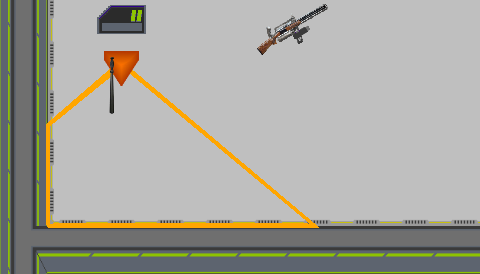
\includegraphics[width=0.835\linewidth]{pics/field-of-view_game.png}
 \captionof{figure}[Visualisierung des Sichtfelds (Version 2)]{Visualisierung des Sichtfelds mit LineRenderer unter Berücksichtigung von Hindernissen.}
	\label{fig:fov2}
\end{figure}

Die Farbe der Linie ist orange für leichte Gegner, rot für Standardgegner und dunkelrot für schwere Gegner. Ob das Sichtfeld visualisiert werden soll oder nicht kann am \texttt{PersonController} eingestellt werden.

\subsubsection{Implementierung des Wahrnehmungssystems}
\label{sec:enemyImplementationAwareness}

Die Wahrnehmung eines Gegners ist mit der Definition seines Sichtfeldes bei weitem nicht abgeschlossen. Die Anwesenheit des Spielers kann nämlich auch auf andere Art und Weise festgestellt werden.

Ein Aspekt ist, dass die Gegner den Spieler 
„hören“ können. Wie das Audiosystem genau funktioniert ist in Kapitel \ref{audio} beschrieben. Außerdem sind beispielsweise die schweren Gegner, wie bereits beschrieben wurde, dazu in der Lage, anderen Gegnern derselben Klasse die aktuelle Position des Spielers mitzuteilen.

Um die Wahrnehmung des Spielers durch den Gegner zu verwalten, wurde für diesen die Komponente \texttt{EnemyAwarenessSystem} implementiert. Diese hat eine Variable namens \texttt{awarenessLevel}, welche einen Wert zwischen null und hundert einnehmen kann und die aktuelle Wachsamkeit des Gegners wiederspiegelt. Externe Einflüsse auf die Wahrnehmung heben diesen Wert an. Dabei wird er beispielsweise durch Sichtkontakt sofort auf hundert angehoben, während er durch Geräusche je nach Lautstärke und Entfernung der Audioqulle unterschiedlich stark verändert wird. 

Die \texttt{Enemy}-Klasse ruft einmal pro \texttt{Update()}-Aufruf die Methode \texttt{IsAboveThreshold} der zugehörigen \texttt{AwarenessSystem}-Komponente ab. Diese Methode gibt an, ob das \texttt{awarenessLevel} über dem Wert der öffentlichen, am Gegner-\textit{Prefab} konfigurierbaren Variable \texttt{attackThreshold liegt.}

Dieser Schwellwert legt fest, wann sich der Status des Gegners ändert: Befindet sich das aktuelle \texttt{awarenessLevel} unter diesem Wert, so patrouilliert der Gegner; befindet es sich über dem Schwellwert, so greift der Gegner den Spieler an.

Damit der Gegner den Spieler nicht dauerhaft weiter verfolgt, gibt es eine Abklingzeit, welche in der Variable \texttt{awarenessCooldown} gespeichert ist. Sobald der Spieler sich nicht mehr im Sichtfeld des Gegners befindet, wird, sofern sie nicht bereits läuft, die \textit{Coroutine} \texttt{AwarenessCooldown()} gestartet, welche das \texttt{awarenessLevel} nach und nach senkt. Sobald der Wert des \texttt{awareness\-Level} wieder unter dem des \texttt{attackThreshold} liegt, wird die Verfolgung abgebrochen.

Die Schwarmintelligenz des schweren Gegners knüpft direkt an das Wahrnehmungssystem an. Hat ein schwerer Gegner den Spieler entdeckt, so wird aus dem \texttt{PersonController}, welcher für die Instanziierung der Gegner zuständig ist, eine Liste der schweren Gegner abgerufen, welche beim \texttt{PersonController} registriert sind. Für jeden dieser Gegner wird das \texttt{awarenessLevel} auf den maximalen Wert gesetzt und die \texttt{lastKnownPlayerPosition} des Gegners auf die aktuelle Position des Spielers. Die schweren Gegner konvergieren daraufhin auf diese Position, aber da der Cooldown für alle Gegner, die nicht in Sichtweite sind, sofort eingeleitet wird, kann es je nach Levelaufbau dennoch für den Spieler möglich sein, zu entkommen, ohne alle schweren Gegner auf einmal bekämpfen zu müssen.

\subsubsection{Implementierung des Gegnertods}
\label{sec:enemyImplementationDeath}

Wird der Gegner durch den Spieler oder durch Fehlschüsse anderer Gegner getroffen, so verliert dieser Lebenspunkte. Ist die Zahl der Lebenspunkte kleiner oder gleich null, so stirbt er.

Der Tod wird folgendermaßen implementiert: Zuerst wird der \textit{Collider2D} des Gegners deaktiviert, sodass er andere Charaktere nicht mehr blockiert. Das Ziel seines \textit{NavAgents} wird auf null gesetzt, sodass er stehen bleibt. Die Waffe wird abgelegt und dann wird durch den \texttt{PersonController} eine Ausblendung eingeleitet, welche damit endet, dass das Spieleobjekt des Gegners zerstört wird. Der \texttt{PersonController} wird deshalb in den Prozess mit einbezogen, weil die Gegner bei ihm registriert sind und damit bei der Weiterentwicklung des Spiels ohne großen Aufwand eine Wiederbelebung implementiert werden kann.

\subsection{Entwicklung des Wegfindungssystems für die Gegner}\label{sec:pathfinding}
Ein zentraler Bestandteil zur Realisierung der künstlichen Intelligenz der Gegner im Spiel ist das Wegfindungssystem. Dieses soll es Gegnern ermöglichen zur Laufzeit des Spiels dynamisch Pfade im Spiellevel zu vorgegebenen Zielpunkten kalkulieren zu lassen und diese schließlich zu traversieren. Ziel des Wegfindungssystems ist es, dass Gegner oder gegebenenfalls auch andere Spielobjekte nur einen Zielpunkt auf dem Level festlegen müssen und die restlichen Berechnungen unabhängig vom Spielobjekt durchgeführt werden.

Hierzu wird zunächst in Abschnitt \ref{sec:pathfindingConcept} das Zusammenspiel und Konzept der zentralen Komponenten genau dargestellt.
Anschließend werden in den Kapiteln \ref{sec:pathfindingAlgo}, \ref{sec:pathProcessing} und \ref{sec:pathCaching} der konkrete Pfadfindealgorithmus, die Pfadnachbearbeitung und die integrierte temporäre Pfadspeicherung zur Performanzverbesserung genauer erläutert. In Kapitel \ref{sec:pathfindingIntegration} wird schließlich behandelt, wie das System bei den Gegnern integriert wird, sodass sie sich im Level fortbewegen und dem Spieler folgen können.

\subsubsection{Grundlegendes Konzept des Systems}\label{sec:pathfindingConcept}
Beim Design der Architektur für das Pfadfindesystem dient die bereits in Unity integrierte Navigationsmechanik \cite{Unity_Doc_Navmesh} als grundlegendes Vorbild. Unity unterteilt die Logik in erster Linie in zwei Komponenten, nämlich in ein \textit{NavMesh} und eine beliebige Anzahl sogenannter Agenten. Das \textit{NavMesh} ist der zentrale Dreh- und Angelpunkt für die Navigation im Level. Es unterteilt das Level abhängig von nicht-passierbaren Hindernissen in begehbare Sektoren in Form von Polygonen und bietet die Funktionalität zur Pfadberechnung auf dem Level. In der Regel existiert pro Szene maximal ein \textit{NavMesh}. Die Agentenkomponente kann zu beliebigen Spielobjekten hinzugefügt werden, die schließlich das \textit{NavMesh} zur Fortbewegung nutzen sollen. In dieser Komponente kann das Bewegungsverhalten außerdem zum Beispiel in Form der Beschleunigung oder Maximalgeschwindigkeit eingestellt werden.

Theoretisch eignet sich das bereits in Unity integrierte System auch für diesen konkreten Anwendungsfall, jedoch ermöglicht eine eigene Implementierung eine optimale Anpassung des Pfadfindungssystems auf die in Kapitel \ref{sec:levelStructure} beschriebene Levelstruktur, da sich der Graph für den Wegfindungsalgorithmus effizient zur Laufzeit berechnen lässt, wie in diesem Kapitel noch genauer erläutert wird. Ebenfalls lässt sich das System so problemlos für zusätzliche Anwendungsfälle im Spiel nutzen. So wird es unter anderem auch zur Entfernungsberechnung von Geräuschen eingesetzt (siehe Kapitel \ref{sec:gegnerreaktionaufaudio}). Aufgrund dessen fällt die Entscheidung darauf, ein eigenständiges Pfadfindungssystem zu realisieren.

\begin{figure}[h]
 \centering
 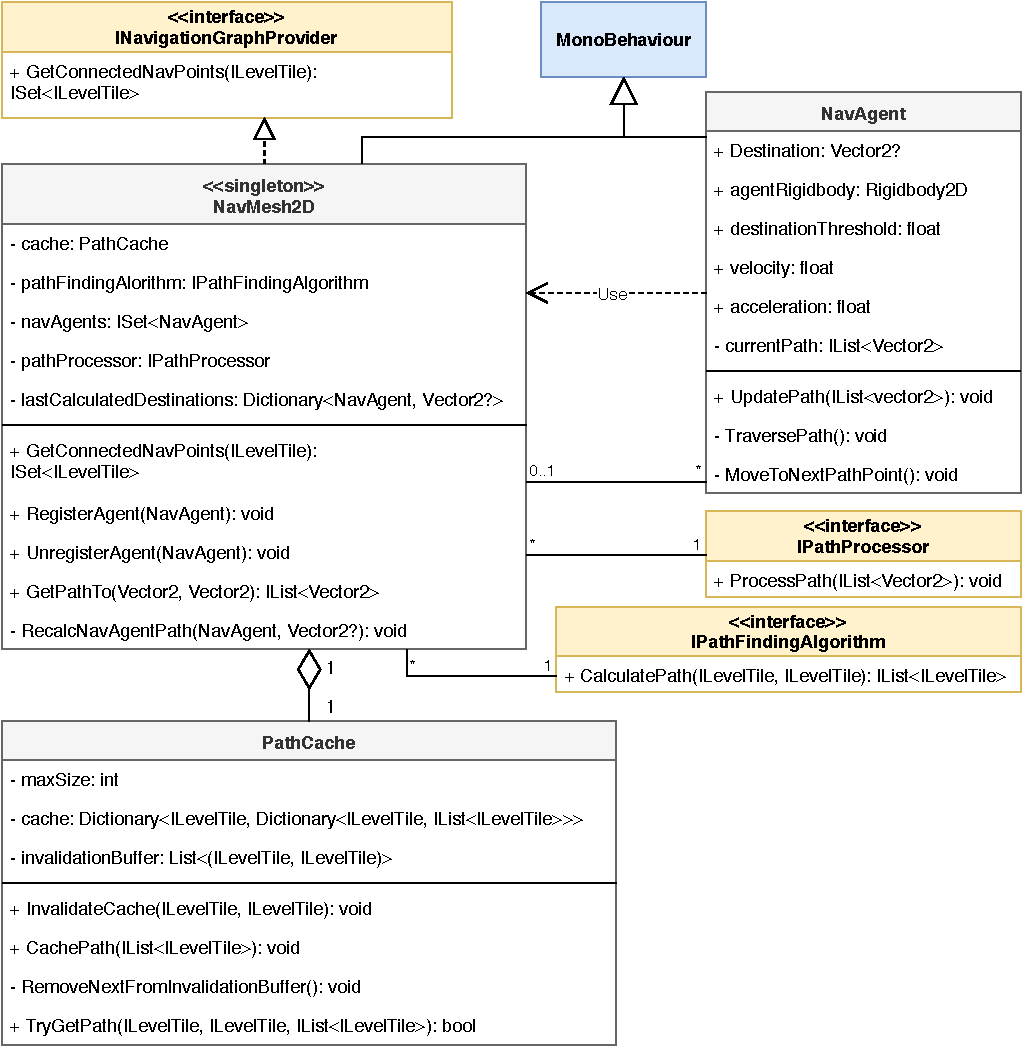
\includegraphics[width=0.835\linewidth]{diagrams/Pathfinding_Structure_reduced.pdf}
 \captionof{figure}[Aufbau des Pfadfindungssystems]{UML-Klassendiagramm der wichtigsten Komponenten des Pfadfindungssystems in vereinfachter Darstellung.}
	\label{fig:pathfinding_structure}
\end{figure}

In der Verwendung unterscheidet sich die Agentenkomponente (\texttt{NavAgent}) kaum vom  Pendant der Unity-Engine, wie in Abbildung \ref{fig:pathfinding_structure} zu sehen ist. Über die \texttt{Destination} lässt sich der momentane Zielpunkt des \texttt{NavAgent} konfigurieren, wobei ein Wert von \texttt{null} indiziert, dass der Agent sich nicht bewegen soll. Ebenso lässt sich die Maximalgeschwindigkeit und die Beschleunigung einstellen. Im Falle der Gegner ist der \texttt{NavAgent} eine Komponente des Spielobjekts und das zentrale Skript der Gegner übernimmt dessen Konfiguration. Der \texttt{NavAgent} hält zudem eine Referenz auf den momentanen Pfad in Form einer Liste von Punkten und traversiert diesen abschnittsweise. Die \texttt{destinationThreshold} definiert dabei, wie nahe sich der Agent an den nächsten Pfadpunkt annähern muss, dass dieser als erreicht gewertet und aus dem aktuellen Pfad entfernt wird. Die Fortbewegung wird dabei durch Anwendung von physikalischen Kräften am \textit{Rigidbody2D} des zugehörigen Spielobjekts in die Richtung des nächsten Pfadpunktes realisiert.

Die Kalkulation des Pfades zum aktuellen Zielpunkt wird an das \texttt{NavMesh2D} ausgelagert. Dieses wird hierzu seitens des \texttt{NavAgent} benachrichtigt, sobald der Wert des Zielpunktes geändert wird, berechnet einen neuen Pfad und aktualisiert den aktuellen Pfad des Agenten über die Methode \texttt{UpdatePath(...)}. Der Agent übernimmt somit de-facto nur die Bewegung des zugehörigen Spielobjekts, während das \texttt{NavMesh2D} für alle Kalkulationen im Hintergrund zuständig ist.

Das \texttt{NavMesh2D} verbindet alle am Pfadfindungssystem beteiligten Komponenten und existiert maximal einmal pro Level. Über die entsprechenden Methoden können sich die Agenten dort registrieren und zum Beispiel nach deren Elimination wieder de-registrieren, wodurch alle Agenten zentral verwaltet werden können. 

Des Weiteren dient das \texttt{NavMesh2D} als die Verbindung zwischen Level und Wegfindealgorithmus, denn die meisten solcher Algorithmen werden auf Basis eines Graphen durchgeführt, während das Level durch die in Kapitel \ref{sec:levelStructure} beschriebene Datenstruktur repräsentiert wird. Hierbei lässt sich die Eigenschaft, dass das Level aus einem Raster von quadratischen Levelteilen besteht und somit inhärent eine Art Graph darstellt, zu Nutze machen. Konkret stellt das \texttt{NavMesh2D} zu diesem Zwecke indirekt den Graphen durch Implementierung des \texttt{INavigationGraphProvider} Interfaces zur Verfügung. Die darin befindliche Methode liefert alle begehbaren und verbundenen Nachbarteile zu einem eingegeben Teil des Levels. Somit kann zum Beispiel der verwendete Wegfindungsalgorithmus des \texttt{NavMesh2D} diese Methode zur Laufzeit nutzen, um Nachbarknoten, beziehungsweise in diesem Fall Nachbarteile, eines aktuell untersuchten Knoten zu ermitteln. Die exakte Vorgehensweise des Algorithmus wird in Abschnitt \ref{sec:pathfindingAlgo} noch genauer erläutert.

\begin{figure}[h]
 \centering
 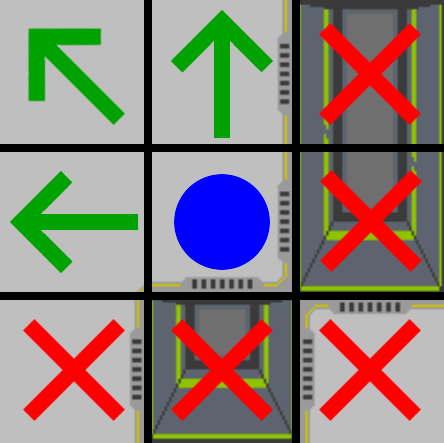
\includegraphics[width=0.4\linewidth]{pics/Graph_Generation.PNG}
 \captionof{figure}[Kalkulation der durch das Pfadfindesystems benutzbaren Levelteile]{Beispielhafte Darstellung der traversierbaren Nachbarteile ausgehend vom momentanen Levelteil (blau markiert) anhand eines Spielausschnitts. Nicht erreichbare Teile sind durch ein rotes Kreuz markiert.}
	\label{fig:graphNeighbourTiles}
\end{figure}

Bei der Berechnung, welche Levelteile durch die \texttt{GetConnectedNavPoints(...)}-Methode als begehbare Nachbarteile zurückgegeben werden, wird die \texttt{IsTraversable()} Funktion des gemeinsamen \texttt{ILevelTile}-Interfaces (siehe Abbildung \ref{fig:level_structure}) aller Levelteile verwendet. Prinzipiell sind alle direkt orthogonal oder diagonal verbundenen Levelteile potenzielle Nachbarn eines Teils, jedoch werden nicht traversierbare herausgefiltert, wie in Abbildung \ref{fig:graphNeighbourTiles} beispielhaft zu sehen ist. Bei diagonal verbundenen Nachbarteilen müssen zudem alle anliegenden orthogonalen Nachbarteile traversierbar sein, ansonsten werden diese Teile ebenfalls ausgeschlossen. Dies ist in Abbildung \ref{fig:graphNeighbourTiles} rechts und links unten beispielhaft zu sehen. Würden diese als begehbar bewertet werden, könnten später berechnete Laufpfade theoretisch direkt an Kanten von Wänden oder ähnlichem verlaufen, wodurch Gegner beim Versuch durch diese zu laufen daran stecken bleiben könnten.

Der Grund, weshalb die Abbildung des Levels als Graph in dieser Form realisiert wird, ist insbesondere, dass so vor Ausführung des Algorithmus nicht a priori ein entsprechender als Eingabe dienender Graph generiert werden muss. Zusätzlich ist dieser Ansatz flexibler gegenüber Änderungen im Level, weil die Nachbarschaftsbeziehungen von Levelteilen erst während der Pfadberechnungen ermittelt werden. Würde der Graph vorher generiert werden, müsste dieser hingegen bei jeder relevanten Änderung aktualisiert werden. Ein mögliches Problem der Kalkulation der verbundenen Graphknoten zur Laufzeit wäre, wenn diese Operation sehr aufwendig zu berechnen ist. In diesem Fall wäre eine vorherige Erzeugung des Graphen der bessere Ansatz. Tatsächlich lassen sich die traversierbaren Nachbarteile mit einer Worst-Case-Laufzeit von \textit{O(1)} berechnen, da die Anzahl möglicher Nachbarteile auf acht begrenzt ist und der Zugriff auf diese ebenso effizient möglich ist. Folglich ist es kein Problem die \texttt{GetConnectedNavPoints(...)}-Methode auch vielfach pro Pfadberechnung aufzurufen.

Das \texttt{NavMesh2D} stellt schließlich über die Methode \texttt{GetPathTo(...)} die Funktionalität zur Berechnung eines Pfades zwischen einem Start- und Endpunkt zur Verfügung. Diese wird zum einen intern zur Neukalkulation der Pfade der registrierten Agenten verwendet und kann zudem auch von externen Komponenten, wie zum Beispiel dem in Kapitel \ref{sec:audiosystem} näher beschriebenen Audiosystem, genutzt werden. Im Gegensatz zum eigentlichen Pfadfindungsalgorithmus liefert das \texttt{NavMesh2D} auch keine Liste von Levelteilen, sondern zweidimensionaler Vektoren als Pfad zurück. Dies liegt in erster Linie daran, dass die Levelteile, wie vorher beschrieben, als Graph für den Algorithmus dienen, die Agenten aber tatsächliche Weltkoordinaten in Form der Vektoren direkt zum Ablaufen der Pfade weiterverwenden können. Intern ruft das \texttt{NavMesh2D} also erst den Wegfindungsalgorithmus vom Levelteil am Startpunkt zum Teil am Endpunkt auf und konvertiert die Liste von Levelteilen schließlich in Weltkoordinaten. Abschließend werden der eigentliche Start- und Endpunkt wieder am generierten Pfad eingefügt und dieser, wie in Abschnitt \ref{sec:pathProcessing} beschrieben, mit dem \texttt{pathProcessor} nachbearbeitet. Der Wegfindealgorithmus liefert also zusammenfassend nur einen Rohpfad, der dann erst für die Weiterverwendung angepasst wird.

Außerdem verfügt das \texttt{NavMesh2D} noch über einen Zwischenspeicher für bereits berechnete Pfade in Form eines \texttt{PathCache}. Dieser dient vor allem dazu, häufige und kostenaufwendige Neukalkulationen von Wegen zu minimieren. Die exakte Funktionsweise wird in Abschnitt \ref{sec:pathCaching} allerdings noch genauer erläutert.

\subsubsection{Umsetzung des Pfadfindealgorithmus}\label{sec:pathfindingAlgo}
Der wichtigste Part des Navigationssystems ist im Kern der Pfandfindealgorithmus. Zwar stellt das \texttt{NavMesh2D} hierzu den Graphen zur Verfügung, jedoch muss durch den Algorithmus noch kalkuliert werden, wie ein Pfad zwischen einem gegebenem Start- und Endpunkt konkret verläuft. Klassischerweise wird zu diesem Zwecke der kürzeste Weg zwischen den beiden Punkten ermittelt.

Für diese Problemstellung existieren zwar zahlreiche Algorithmen, allerdings ist die Effizienz dieser für die Performanz des Spiels von ausschlaggebender Bedeutung, da die Berechnung kürzester Wege zumindest CPU-seitig zu den aufwendigeren Operationen zählt. Außerdem müssen die Pfade im ungünstigsten Fall für viele Gegner gleichzeitig ermittelt, und in kurzen Intervallen neu kalkuliert werden.

Zur Lösung dieser Probleme wird hierzu, vor allem auch in der Videospielentwicklung, sehr häufig der sogenannte \textit{A-Star Algorithmus} \cite{A_Star_Paper} angewendet. Dieser ist zwar prinzipiell nicht zwangs\-läu\-fig schneller, als zum Beispiel \textit{Dijkstras Algorithmus} \cite[658]{cormen}, kann aber in der realen Anwendung oft eine deutliche Beschleunigung bei Pfadberechnungen erzielen. Grund hierfür ist, dass A-Star folgende Voraussetzungen bei der Kalkulation gezielt ausnutzt:
\begin{itemize}
	\item Es existiert nur ein konkretes, bekanntes Ziel, zu dem der kürzeste Weg ermittelt werden soll.
	\item Die geschätzten Kosten zum Ziel lassen sich effizient von jedem Graphknoten aus berechnen.
\end{itemize}
Im Kern funktioniert der A-Star Algorithmus sehr ähnlich zu Dijkstras Algorithmus. Es werden vom aktuellen Knoten ausgehend Schrittweise jeweils die Nachbarknoten darauf untersucht, ob der Weg zu diesem Knoten kürzer ist, als der vorher eingetragene. Ist der untersuchte Knoten der Zielknoten, wird die Suche abgebrochen und der Weg zum Zielknoten zurückgegeben. Die als nächstes zu betrachtenden Knoten werden in einer Prioritätswarteschlange nach ihrer Distanz vom Startknoten aufsteigend eingeordnet und in dieser Reihenfolge durch den Algorithmus untersucht. Dies ist der Punkt, in dem der A-Star Algorithmus in der Vorgehensweise hauptsächlich von Dijkstras Algorithmus divergiert. Hier werden in der Prioritätswarteschlange die Kosten zu diesem Knoten plus die geschätzten Kosten zum Zielknoten verwendet (siehe \cite[S. 102]{A_Star_Paper}). Konkret bedeutet dies, dass bei A-Star neben Knoten, die möglichst nah am Startknoten liegen, außerdem auch Knoten, die geschätzt eine kurze Distanz zum Zielknoten haben, bevorzugt untersucht werden. Während Dijkstras Algorithmus also einfach stückweise die günstigsten Wege unabhängig von deren Richtung ermittelt, bis der Zielknoten erreicht ist, arbeitet A-Star von Anfang an zielgerichtet und kann so in den meisten Fällen die Zahl der benötigten Operationen deutlich verringern, obwohl es sich nach wie vor um einen Greedy-Algorithmus handelt. Dies ermöglicht A-Star innerhalb dieses Spiels zum Beispiel auf Flächen ohne Obstruktionen sofort einen kürzesten Weg zu finden, ohne unnötige Knoten innerhalb des Algorithmus zu expandieren.

Der entscheidende Faktor, ob der A-Star Algorithmus verwendet werden kann, beziehungsweise wie effizient dieser funktioniert, ist die sogenannte \textit{Heuristik}, die verwendet wird, um die Distanz von einem Knoten zum Zielknoten zu schätzen. Neben der bereits vorher genannten Anforderung, dass die Schätzung effizient durchgeführt werden können muss, sind folgende weitere Kriterien zu berücksichtigen:
\begin{itemize}
	\item Für keinen Knoten dürfen die geschätzten Kosten zum Ziel größer als die geschätzten Kosten eines Nachbarknotens zum Zielknoten plus die Kosten zu diesem Nachbarknoten sein \cite[S. 98]{ai_modern_approach}. Dies wird in der Heuristik auch \textit{Konsistenzkriterium} genannt. Ist dieses nicht erfüllt, ist auch das Optimalitätskriterium für den Algorithmus nicht mehr gegeben, was bedeutet, dass der Algorithmus bei Existenz eines Weges zum Ziel zwar terminiert, aber nicht zwangsläufig den kürzesten Weg zurückgibt.
	\item Die Heuristik sollte die Kosten im Optimalfall so schätzen, dass die Differenz zu den realen Kosten möglichst gering ist, denn durch eine genauere Schätzung sind im Durchschnitt weniger Rechenschnitte notwendig \cite[S. 98]{ai_modern_approach}.
\end{itemize}
Eine vor allem in der Spielentwicklung beliebte Heuristik ist die euklidische Distanz zwischen zwei Punkten, da die Navigation meist ohnehin in einem geometrischen Raum ausgeführt wird und die euklidische Distanz ein zuverlässiger Indikator für den Mindestabstand einer Verbindung zwischen zwei Punkten ist. Zudem erfüllt diese Heuristik aufgrund der Gültigkeit der Dreiecksungleichung im geometrischen Raum das Konsistenzkriterium und ist zudem schnell mit Laufzeit \textit{O(1)} durch die Berechnung des Abstands zweier Vektoren ermittelbar. Aus den genannten Gründen wird die euklidische Heuristik auch innerhalb dieses Projekts für den A-Star Algorithmus eingesetzt.

Für die Prioritätswarteschlange, in der die als nächstes zu expandierenden Knoten gehalten werden, wurde ein Fibonacci-Heap implementiert. Der Grund für die Verwendung dieser speziellen Form eines Heaps ist, dass dieser eine Laufzeit für das Einfügen neuer Elemente von \textit{O(1)} bietet \cite[S. 511]{cormen}, im Gegensatz zu \textit{O(log(n))} beispielsweise bei einem binären Heap \cite[S. 164]{cormen}. Dies ist in diesem Fall insofern relevant, dass jedes Teil im Level bis zu acht begehbare Nachbarteile besitzen kann, welche in den Heap eingefügt werden müssen. Ebenso kann in einem Fibonacci-Heap der Schlüssel eines Elements in konstanter Laufzeit verringert werden \cite[S. 518]{cormen}, was beim A-Star Algorithmus konkret bei der Relaxierung von Kanten geschieht. Tatsächlich ist dieser theoretische Vorteil hier nahezu irrelevant, da aufgrund der Gültigkeit der Dreiecksungleichung der direkte Weg zwischen zwei Knoten auch immer der Kürzeste ist, was de-facto dazu führt, dass keine Kanten zu einem Knoten relaxiert werden, nachdem das erste Mal ein kürzester Weg zu diesem gefunden wurde. Aufgrund der schnellen Laufzeit beim Einfügen von Elementen bietet sich ein Fibonacci-Heap dennoch als Datenstruktur an. Nebenbei ist anzumerken, dass das Entfernen des Minimums aus dem Fibonacci-Heap theoretisch ein Problem für die Performanz sein könnte, da nur in der amortisierten Analyse eine sehr schnelle Laufzeit von \textit{O(log(n))} gegeben ist. Das bedeutet, dass diese Operation in Ausnahmefällen auch eine deutlich schlechtere Zeitkomplexität hat, was zu einem unflüssigen Spielerlebnis führen könnte. In der realen Anwendung sind solche Performanzeinbrüche jedoch nicht zu beobachten, auch wenn mehrere längere Pfade berechnet werden müssen.

\subsubsection{Pfadverarbeitung für die Verwendung bei den Gegnern}\label{sec:pathProcessing}
Mithilfe des A-Star Algorithmus lassen sich soweit effizient auf Levelteilen basierend kürzeste Pfade berechnen, jedoch lassen sich diese durch entsprechende Nachbearbeitung besser durch die Navigationsagenten nutzen. Aktuell führt das \texttt{NavMesh2D} folgende zwei Bearbeitungsschritte durch:
\begin{itemize}
	\item Entfernen von \textit{Backtracking} (siehe Abbildung \ref{fig:backtrackingPath}) am Start und Ende des Pfades.
	\item Entfernen unnötiger Pfadpunkte. Dies sind Wegpunkte, die auf einer direkten Linie zwischen zwei anderen Pfadpunkten liegen, und somit keine zusätzliche relevante Information zur Navigation darstellen.
\end{itemize}

\begin{figure}[h]
 \centering
 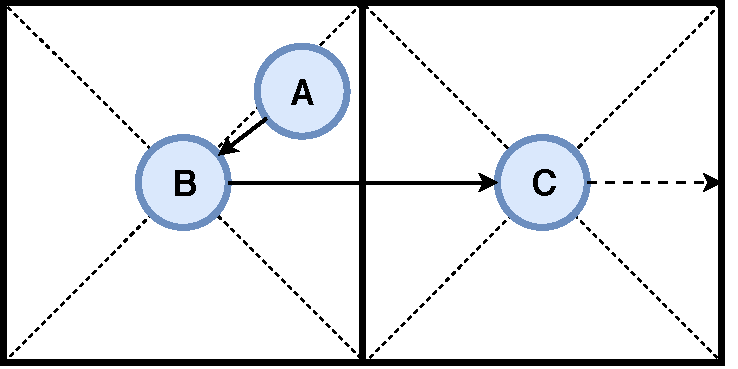
\includegraphics[width=0.4\linewidth]{pics/Backtracking_Example.pdf}
 \captionof{figure}[Beispiel für \textit{Backtracking} am Anfang eines Pfades]{Beispiel für \textit{Backtracking} am Anfang eines Pfades zwischen den Punkten A, B und C.}
	\label{fig:backtrackingPath}
\end{figure}

Erstere Operation ist vonnöten, da der tatsächliche Start- und Endpunkt des Pfades nach Berechnung des teilebasierten Pfades noch eingefügt wird. Dies kann dazu führen, dass zum Beispiel am Start ein Pfad zurückführt, obwohl dieser dann in eine andere Richtung verläuft, wie beispielhaft in Abbildung \ref{fig:backtrackingPath} zu sehen. Dort ist der Punkt A der tatsächliche Startpunkt, während Punkt B und C teil des vom Pfadfindealgorithmus kalkulierten Pfades sind. In einem solchen Fall wird der mittlere Knoten, also hier B, aus dem Pfad entfernt, um beim Agenten später unnötige Bewegungen zu vermeiden. Am Ende des Pfades wird analog verfahren.

\begin{figure}[h]
 \centering
 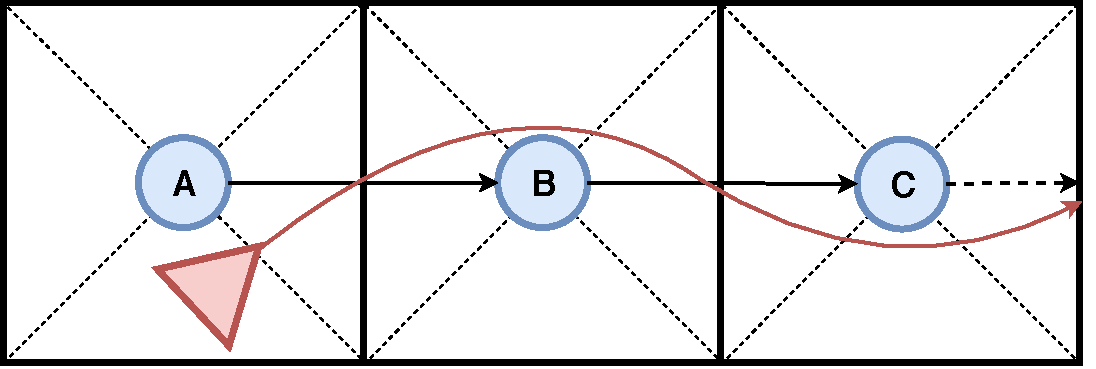
\includegraphics[width=0.6\linewidth]{pics/Enemy_Path_Oscillation.pdf}
 \captionof{figure}[Oszillierende Pfadabweichung von Gegnern bei vielen Pfadpunkten]{Beispielhafte Darstellung der oszillierenden Pfadabweichung von Gegnern (rot dargestellt) auf einem geraden Pfad mit vielen Knotenpunkten.}
	\label{fig:enemyOscillation}
\end{figure}

Die zweite genannte Pfadnachbearbeitung führt ebenso zu einem besseren Bewegungsverhalten bei den Agenten. Das grundlegende Problem ist, dass die Agenten durch die Anwendung physikalischer Kräfte bewegt werden und so in der Bewegung träge sind. Dies ist zwar prinzipiell bewusst so gewählt, um die Bewegung flüssig erscheinen zu lassen, jedoch bleibt zum Beispiel auf einer geraden Strecke die laterale Geschwindigkeit erhalten. Das bedeutet, dass der Agent sich beim Ablaufen des Pfades zwischen den Pfadpunkten seitlich hin- und herbewegen kann, wie in Abbildung \ref{fig:enemyOscillation} skizziert ist. Der beschriebene Effekt ist zwar nur subtil, lässt die Bewegung der Agenten allerdings unnatürlich aussehen. Durch die Entfernung unnötiger Pfadpunkte (in der Abbildung entspricht dies B) lässt sich dieser Effekt vermeiden und der Pfad an sich wird ohne relevanten Informationsverlust vereinfacht.

Beide der genannten Pfadverarbeitungsoperationen könnten theoretisch in Form von Methoden des \texttt{NavMesh2D} realisiert werden. Um eine bessere Wiederverwendbarkeit und Flexibilität des Systems zu gewährleisten, wird die Pfadbearbeitung jedoch mithilfe des \textit{Decorator}-Entwurfsmusters \cite[175]{Design_Patterns} umgesetzt. Jede Klasse die das \texttt{IPathProcessor} Interface implementiert (siehe Abbildung \ref{fig:pathfinding_structure}), kann über den Konstruktor einen weiteren \texttt{IPathProcessor} übergeben bekommen. Bei Aufruf der \texttt{ProcessPath(...)}-Methode wird dann erst die selbe Methode beim übergebenen \texttt{IPathProcessor} aufgerufen, sofern vorhanden. So kann ein Pfadverarbeiter individuell konfiguriert werden. Das \texttt{NavMesh2D} erzeugt schließlich beim Start der Spielszene einen entsprechenden Pfadverarbeiter, der dann auf allen vom Wegfindealgorithmus errechneten Pfaden angewandt wird.

\subsubsection{Pfadspeicherung zur Performanzverbesserung}\label{sec:pathCaching}
Durch Verwendung des A-Star Algorithmus in Kombination mit Fibonacci-Heaps lassen sich Pfadberechnungen bereits sehr performant durchführen. Dennoch ist es sinnvoll die Effizienz wenn möglich weiter zu verbessern, da in keiner Weise festgelegt ist, wie viele Gegner gleichzeitig pro Level aktiv sein können. Folglich lässt sich aus einer guten Performanz in den getesteten Leveln kein allgemeiner Schluss ziehen. Deshalb wird zusätzlich ein Pfadspeicherungssystem integriert, welches vom \texttt{NavMesh2D} genutzt wird und kürzlich berechnete Pfade zwischenspeichert.

Der in Abbildung \ref{fig:pathfinding_structure} dargestellte \texttt{PathCache} wird bei Start der Spielszene durch das \texttt{NavMesh2D} erzeugt. Dabei wird im Konstruktor die maximale Anzahl gleichzeitig zwischengespeicherter Pfade spezifiziert. Der Speicher an sich ist durch ein zweifach verschachteltes \texttt{Dictionary} umgesetzt, bei dem das Start- und Endteil des Pfades jeweils den Schlüssel darstellen und der Pfad an sich den Wert des inneren \texttt{Dictionary}. Dies ermöglicht die Abfrage von Pfaden mit der \texttt{TryGetPath(...)}-Methode in konstanter Laufzeit über je eine Hash-Suche des Start- und Endpunktes. Über die \texttt{CachePath(...)}-Methode lassen sich Pfade zum Speicher hinzufügen. Gegensätzlich lassen sich durch Aufruf von \texttt{InvalidateCache(...)} Wege wieder aus dem Speicher entfernen.

Ein Problem des Systems ist, dass die Anzahl möglicher Pfade quadratisch mit der Anzahl an Levelteilen wächst. Würden also alle berechneten Pfade gespeichert werden, würde dies rasch eine substanzielle Menge an Arbeitsspeicher in Anspruch nehmen. Deshalb wird bei erreichen der Speicherkapazität \texttt{maxSize} bei Speicherung eines Pfades ein anderer nach dem Prinzip \textit{Least Recently Used} aus dem Pfadspeicher verdrängt. Zu diesem Zweck führt der \texttt{invalidationBuffer} mit, in welcher Reihenfolge die Pfade zuletzt verwendet wurden. Wird ein Weg aus dem Speicher abgefragt, wird dieser wieder an den Anfang des Puffers gesetzt. Bei Überschreitung der Maximalgröße wird dann das letzte Element entfernt. Die Pfade werden im \texttt{invalidationBuffer} als Tupel aus Start- und Endpunkt gehalten.

Das \texttt{NavMesh2D} prüft nun vor der Pfadberechnung erst, ob der gesuchte Pfad bereits im Speicher ist. Nur wenn dies nicht der Fall ist, wird tatsächlich der Wegfindealgorithmus aufgerufen und das Ergebnis schließlich im \texttt{PathCache} abgelegt. So lassen sich durch geringfügig höheren Arbeitsspeicherverbrauch viele aufwendige Pfadberechnungen verhindern. Vor allem die Wege zwischen den Patroullienpunkten von Gegnern müssen so in der Regel nur ein einziges Mal bei Levelstart kalkuliert werden und sind von diesem Zeitpunkt an im Speicher abgelegt.

\subsubsection{Integration des Wegfindungssystems in das Gegnerverhalten}\label{sec:pathfindingIntegration}
Nachdem das Pfadfindungssystem soweit funktional und effizient ist, muss es schließlich noch in die Gegner integriert werden. Hierzu hat jeder Gegner eine \texttt{NavAgent}-Komponente. Diese wird standardmäßig genutzt, um die Patrouillienpunkte abzulaufen, indem immer der Nächste als aktuelles Ziel des Agenten gesetzt wird.

\begin{figure}[h]
 \centering
 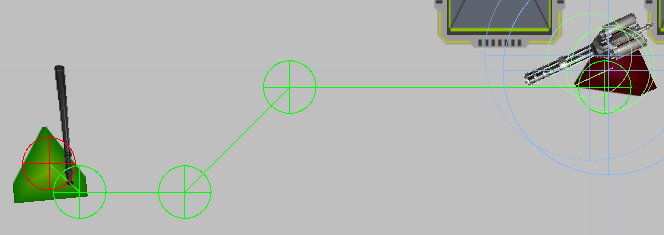
\includegraphics[width=0.7\linewidth]{pics/path_gizmo.png}
 \captionof{figure}[Debug-Anzeige für Gegnerpfade]{Debug-Anzeige des aktuellen Pfades eines Gegners. Die Pfadpunkte werden dabei als Kreise dargestellt.}
	\label{fig:pathGizmo}
\end{figure}

 Um das Debuggen zu erleichtern, werden die aktuellen Routen der Gegner bei Auswahl in der Szene als sogenannte \textit{Gizmo}s angezeigt. Dies sind Elemente, die nur innerhalb des Unity Editors angezeigt werden können, um zusätzliche visuelle Information zu Spielobjekten zu erhalten. In Abbildung \ref{fig:pathGizmo} ist die Debug-Ansicht eines Gegnerpfades beispielhaft abgebildet.

Neben dem Ablaufen von Patrouillienpunkten ist das Verhalten der Gegner, sobald der Spieler entdeckt wurde, deutlich komplexer. In diesem Fall soll der Spieler verfolgt werden und solange die Aufmerksamkeit der Gegner über dem Angriffsschwellwert liegt, gegebenenfalls aktiv gesucht werden. Da das Suchverhalten der Gegner von Typ zu Typ variieren soll, wird hierfür das Decorator-Entwurfsmuster \cite[175]{Design_Patterns} eingesetzt, wie in Abbildung \ref{fig:followBehaviourUML} dargestellt. So wird verhindert, dass für jeden Gegnertyp eine Unterklasse mit individuellem Verhaltensmuster erstellt werden muss. Stattdessen wird das Verhalten bei Erzeugung der Gegner erstellt und diesen schließlich zugewiesen und kann so je nach Typ konfiguriert werden.

\begin{figure}[h]
 \centering
 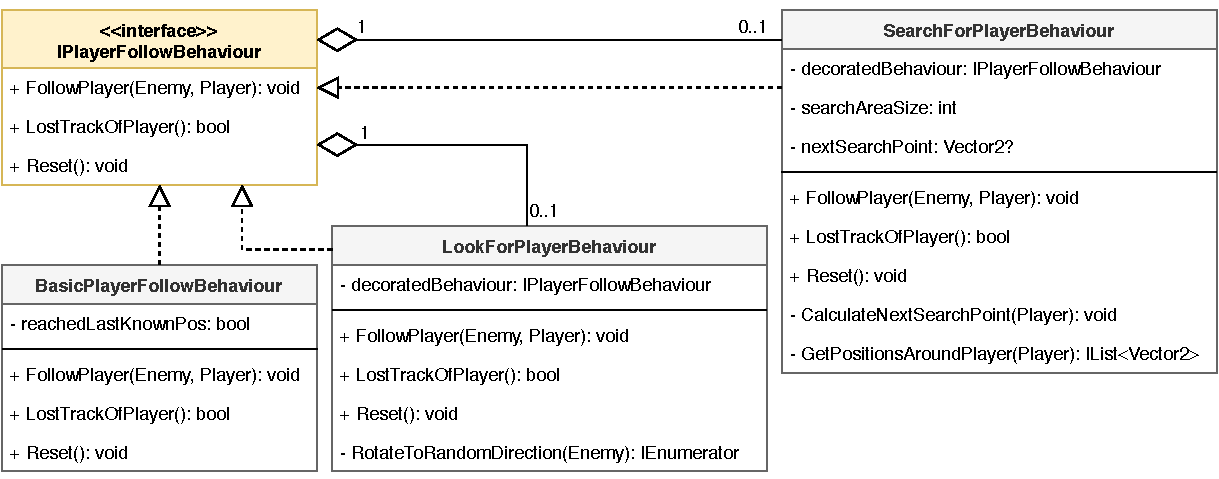
\includegraphics[width=1\linewidth]{diagrams/Player_Follow_Behaviour_UML.pdf}
 \captionof{figure}[Decorator für das Spieler-Suchverhalten der Gegner]{UML-Diagramm für das Spieler-Suchverhalten der Gegner.}
	\label{fig:followBehaviourUML}
\end{figure}

Das Interface für das Verfolgungs- beziehungsweise Suchverhalten der Gegner beinhaltet folgende drei Grundfunktionen, die durch alle Unterklassen implementiert werden müssen:

\begin{itemize}
	\item\textbf{\texttt{FollowPlayer(...)}:} Signalisiert der Verhaltensklasse, dass der Gegner dem Spieler folgen soll. Diese Methode wird zyklisch durch den Gegner aufgerufen, solange dessen Aufmerksamkeitslevel über dem Angriffsschwellwert ist.
	\item\textbf{\texttt{LostTrackOfPlayer()}:} Diese Methode gibt einen boolschen Wert zurück der angibt, ob der Gegner die Spur des Spielers verloren hat.
	\item\textbf{\texttt{Reset()}:} Diese Methode wird durch den Gegner aufgerufen, sobald dieser wieder zum Normalverhalten zurückkehrt und kann durch die konkreten Verhaltensklassen genutzt werden, um sich auf den Anfangszustand zurückzusetzen.
\end{itemize}

Alle Unterklassen, abgesehen vom \texttt{BasicPlayerFollowBehaviour}, müssen innerhalb der Inter\-face-Methoden jeweils auch die Methode des dekorierten Verhaltens aufrufen. So lässt sich das Verhalten durch jede spezifische Implementierung stückweise erweitern, ohne die Funktionalität der anderen abzuändern.

Das \texttt{BasicPlayerFollowBehaviour} ist der Grundbaustein für das Suchverhalten aller Gegner. Es setzt im Agenten des Gegners die letzte bekannte Position des Spielers als Ziel und folgt diesem so direkt. Die letzte bekannte Position ist die Stelle, an der der Spieler zuletzt durch den Gegner gesehen oder gehört wurde. Sobald dieser Punkt erreicht ist, gibt die \texttt{LostTrackOfPlayer()}-Methode auch \texttt{true} als Rückgabewert zurück. Dies wird durch die anderen Verhaltensunterklassen als Signal gewertet, weitere Suchmaßnahmen einzuleiten.

Das \texttt{LookForPlayerBehaviour} lässt den Gegner schließlich nach Erreichen der letzten bekannten Spielerposition, randomisiert in verschiedene Richtungen blicken, um so zu versuchen erneuten Sichtkontakt zum Spieler wiederherzustellen. Die Koroutine \texttt{RotateToRandomDirection()} übernimmt dabei das Rotieren des Gegners.

Weil schwerere Gegner nach Verlust der Spur des Spieler zusätzlich noch aktiv die Umgebung absuchen sollen, wird zu diesem Zweck bei diesen noch das \texttt{SearchForPlayerBehaviour} eingesetzt. Bei der Umsetzung ist entscheidend, ob die Gegner tatsächlich direkt zum Spieler navigieren sollen, also de-facto immer dessen Position kennen, oder uninformiert und somit theoretisch realistischer die Gegend beispielsweise randomisiert absuchen sollen. Konkret wird eine Kompromisslösung aus den beiden Ansätzen gewählt, sodass Gegner mit diesem Suchverhalten nicht immer direkt zum Spieler laufen, aber trotzdem gezielt in dessen Nähe nach diesem suchen, um so eine Balance aus Realismus und Herausforderung zu schaffen. Hierzu wird im Umkreis um den Spieler zufällig ein begehbares Levelteil ausgewählt und als Ziel des Navigationsagenten des Gegners gesetzt. Bei Erreichen dieses Punktes wird solange erneut ein solcher zufälliger Punkt gewählt, bis das Aufmerksamkeitslevel des Gegners unter den Angriffsschwellwert fällt. Die \texttt{searchAreaSize} gibt an, in welchem Umkreis in Form von Teilen um den Spieler Suchpunkte ausgewählt werden können. Ein geringerer Wert bedeutet also, dass der Gegner zielgenauer nach dem Spieler sucht. Dies ermöglicht, dass die Gegner zwar durchaus aktiv und relativ zielgerichtet suchen, durch die Ungenauigkeit aber dem Spieler dennoch die Möglichkeit einräumen zu entkommen.
\pagebreak

% Audio
\section{Audio} \label{audio}
Geräusche und Musik im Spiel sind ein wesentlicher Bestand, denn es erhöht die Erlebnisqualität und gibt jedem Spiel einen eigenen Charakter. Geräusche ermöglichen es dem Spieler außerdem zusätzliche Informationen wie beispielsweise die Entfernung und Richtung aus der er einen Gegner erwarten kann, zu erhalten. 

\subsection{Wichtige Komponenten in Unity}
Um Töne in Unity abzuspielen, sind folgende Komponenten notwendig:

\begin{itemize}
	\item \textit{AudioListener}: Komponente, bei der Töne empfangen werden.
	\item \textit{AudioSource}: Komponente, die Töne abspielt. 
\end{itemize}

Damit näher in der Umgebung entstehende Geräusche auch lauter sind als weiter entfernte und der Spieler Geräusche aus einer bestimmten Richtung orten kann, müssen Einstellungen bei jeder \textit{AudioSource} gemacht werden. Durch diese Einstellungen und der Entfernung der \textit{AudioSource} vom \textit{AudioListener} ist es Unity möglich, die Richtung und Lautstärke für die Entfernung des Spielers zum Geräusch genau zu berechnen. Diese Informationen werden dem physikalischen Soundsystem des Spielers mitgeteilt, sodass der Nutzer auch hören kann, aus welcher Richtung das Geräusch entstammt.

Um es dem Benutzer zu ermöglichen Geräusche verschiedener Kategorien, wie beispielsweise die Hintergrundmusik oder die Soundeffekte unterschiedlich einzustellen, werden sogenannte \textit{AudioMixer} und \textit{AudioMixerGroups} benötigt. Abbildung \ref{fig:audio_routing} zeigt das Zusammenspiel dieser Komponenten für den aktuellen Projektstand.

\begin {figure}[h]
	\begin {center}
	    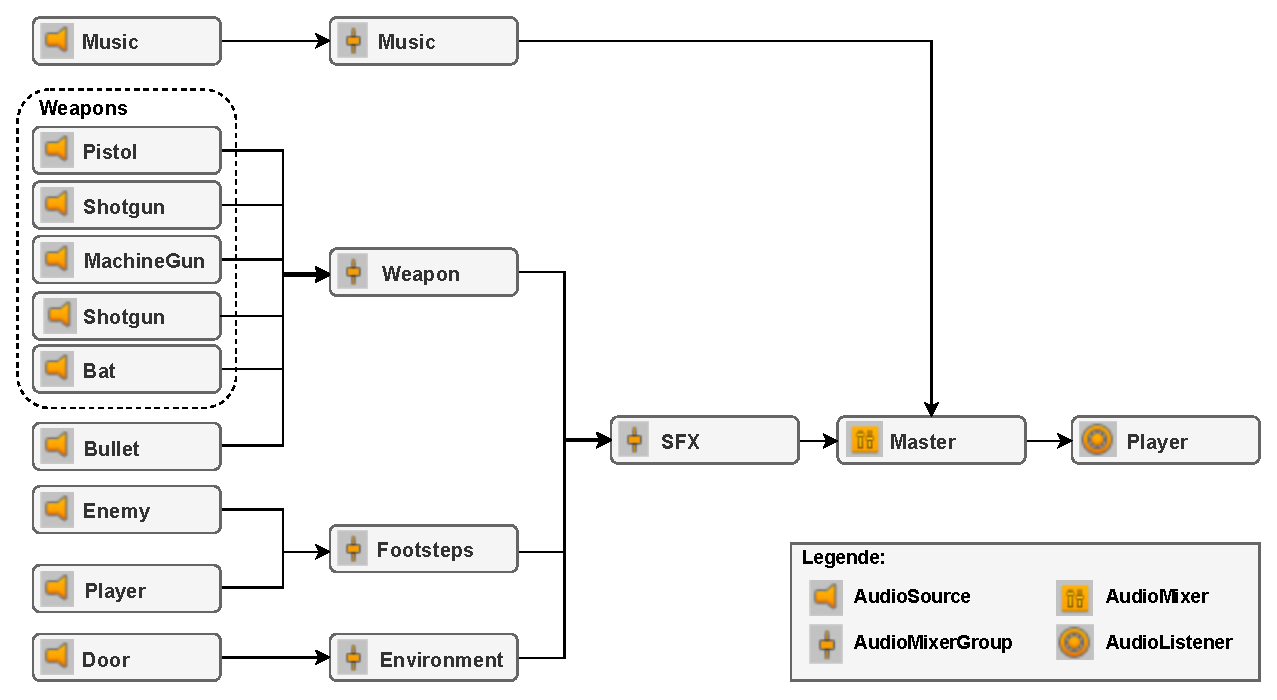
\includegraphics[width=1\textwidth]{pics/audio_routing.eps}
		\caption{Weiterleitung der Audiosignale}
		\label{fig:audio_routing}
	\end {center}
\end {figure}

Falls keine \textit{AudioMixer} und AudioMixerGruppen (\textit{AudioMixerGroups}) eingestellt sind, werden Töne direkt von der \textit{AudioSource} zum \textit{AudioListener} geleitet. Für jede \textit{AudioSource} kann eingestellt werden, zu welcher \textit{AudioMixerGroup} diese die Töne weiterleiten soll. Für einen \textit{AudioMixer} können dabei beliebig viele AudioMixerGruppen eingerichtet werden. Durch eine Hierarchie kann festgelegt werden, zu welcher übergeordneten AudioMixerGruppe eine bestimmte \textit{AudioMixerGroup} empfangene Töne weiterleitet. Standardmäßig existiert bereits bei Erstellung eines \textit{AudioMixers} eine \textit{AudioMixerGroup}: Der \textit{Master}. Da alle Tonsignale des \textit{AudioMixers} an diese Gruppe weitergeleitet werden, kontrolliert diese die Gesamtlautstärke. Ist für einen \textit{AudioListener} ein \textit{AudioMixer} eingestellt, so leitet die \textit{Master}-Gruppe eines \textit{AudioMixers} die Tonsignale an diesen weiter.
 
\subsection{Das Audiosystem}\label{sec:audiosystem}
Damit ein Spieler hören kann, wie weit ein Gegner entfernt ist und aus welcher Richtung er kommt, müssen folglich die Töne von Gegnern immer genau dort entstehen, wo sich die Gegner gerade befinden. Daher muss jeder Gegner eine eigene Audioquelle besitzen.

Damit eine Audioquelle (\textit{AudioSource}) Töne abspielen kann, muss ihr diese sogenannte Tonspur (\textit{AudioClip}) übergeben und die Methode \texttt{Play()} der Audioquelle aufgerufen werden. Die im Projekt verwendeten \textit{AudioClips}\cite{KompositeSoundCaesarBostonProfiDevelopers.2019} sind vom \textit{Asset Store}\cite{Unity_Doc_Assets_Bib} importiert worden. Zu jeder Tonspur gibt es Eigenschaften wie beispielsweise die Lautstärke, die \textit{AudioMixerGroup}, an die die Tonsignale weitergeleitet werden sollen oder, ob der \textit{AudioClip} in einer Endlosschleife gespielt werden soll. All diese Eigenschaften werden zusammen mit dem \textit{AudioClip} in einer eigenen Klasse \texttt{Sound}\ref{fig:audio_system} gespeichert. Neben Eigenschaften, die jeder \textit{AudioClip} besitzt, gibt es zwei verschiedene Situationen, in denen Geräusche entstehen und somit eine Unterteilung in zwei verschiedene Kategorien erforderlich machen: 

\begin{enumerate}
	\item Die Töne entstehen an bestimmten Orten im Spiel.
	\item Es gibt keinen bestimmten Ort im Spiel, von dem aus die Tonspur abgespielt wird.
\end{enumerate}

Die mit Abstand meisten Tonspuren müssen an bestimmten Orten abgespielt werden. Wird beispielsweise eine Waffe abgefeuert, so entsteht ein hörbares Geräusch genau bei der Waffe, ein Geräusch während dem Fliegen der Kugel und ein weiteres Geräusch genau bei dem Einschlagspunkt des Geschosses. Für das Spiel wurde zweiteres weggelassen, da zu viele Geräusche ein Spieler als störend empfinden würde, dieses im Spiel klar zu sehen ist und somit keine zusätzlichen Informationen liefert. Zudem muss beachtet werden, dass eine bestimmte Waffe im Spiel mehrfach vorhanden sein, von unterschiedlichen Positionen aus zeitlich versetzt voneinander abgefeuert werden kann, mehrere Geschosse des gleichen Typs zur gleichen Zeit existieren und auch zeitlich als auch örtlich unterschiedliche Einschlagspunkte haben können. Zu diesen Tonspuren müssen weitere Eigenschaften definiert werden, die es dem Spieler ermöglichen sowohl die Richtung als auch die Nähe von entstehenden Geräuschen einschätzen zu können.

Zum zweiten Fall gehört beispielsweise die Hintergrundmusik. All die Fälle, die zu dieser Gruppe gehören, haben zudem die Eigenschaft, dass die gleiche Tonspur nie gleichzeitig abgespielt wird. Denn der Spieler würde dies als störend empfinden. Somit kann jede Tonspur in dieser Gruppe einer einzelnen Audioquelle zugeordnet werden.

Da die Tonspuren für diese zwei Fälle unterschiedliche zusätzliche Eigenschaften benötigen, wurde eine Klasse \texttt{DynamicSound} für örtlich positionierte und eine andere Klasse \texttt{StaticSound} für synchron und ohne bestimmten Ort abzuspielende Tonspuren entworfen. Diese erben von der abstrakten Klasse \texttt{Sound}. 

Um in Unity verwendet werden zu können, muss nun zunächst für jede Tonspur eine Instanz einer der beiden Klassen erstellt und die Eigenschaften für die Tonspuren individuell angepasst werden. Dies muss möglich sein, da die Tonspuren bereits bei Erstellung unterschiedliche Lautstärken haben können. Ein sehr großer Vorteil, der sich daraus ergibt ist, dass die gleiche Tonspur für mehrere Situationen verwendet werden und somit der Entwicklungsaufwand deutliche reduziert werden kann. Wird beispielsweise eine schallgedämpfte Pistole implementiert, so kann die Tonspur der Pistole wiederverwendet und vor allem die Lautstärke dieser Tonspur und anderer Eigenschaften verändert werden. Diese eingestellten Sound-Objekte dienen dazu im Spiel Audioquellen von Spielobjekten zu konfigurieren und werden daher im nachfolgenden als \glqq{Konfigurationsobjekte\grqq{} bezeichnet.

\subsubsection{Designmöglichkeiten}
Die zentrale Rolle des zu entwerfenden Audiosystems ist es nun, diese Konfigurationsobjekte zu verwalten. Grundsätzlich gibt es hierfür zwei Implementierungsmöglichkeiten:

\begin{itemize}
	\item Eine zentrale Klasse verwaltet alle Konfigurationsobjekte und übergibt auf Anfrage eine Referenz auf das angefragte Objekt.
	\item Jedes \textit{Prefab} verwaltet die zu es gehörenden Konfigurationsobjekte.
\end{itemize}

In Unity ist es üblich solche bereits vor Laufzeit vorhandenen Objekte in einer Liste zu speichern. Alle Konfigurationsobjekte in einer zentralen Klasse in einer Liste zu speichern, würde dazu führen, dass diese schnell anwächst und somit zu folgenden Problemen:

\begin{enumerate}
	\item Änderungen an Einstellungen der Konfigurationsobjekte sind schlecht durchführbar, da das richtige Konfigurationsobjekt erst unter allen in der Liste gespeicherten Objekten gesucht werden muss. 
	\item Um eine Tonspur abzuspielen, muss immer unter allen existierenden Konfigurationsobjekten gesucht werden. Mit der Häufigkeit des Abspielens von Geräuschen ist dies ein bedeutender Faktor. 
	\item Im Code muss für jedes machbare Geräusch eines Spielobjektes speziell das dazugehörige Konfigurationsobjekt zum Abspielen angegeben werden. Da die zentrale Komponente alle Sounddateien besitzt, kann sie beispielsweise mit dem Befehl \glqq{}Waffe abfeuern\grqq{} nicht genau zuordnen, ob die Tonspur von dem Maschinengewehr oder der Pistole abgespielt werden soll.
\end{enumerate}

Durch eine geeignete Datenstruktur kann der Aufwand zum Suchen des richtigen Konfigurationsobjektes verringert werden. Dennoch ist dieser Aufwand größer, als wenn jedes \textit{Prefab} bereits die Konfigurationsobjekte besitzt, die es benötigt. 

\begin{itemize}
	\item Dadurch muss nur unter den für das Spielobjekt benötigten Konfigurationsobjekte gesucht werden, um das richtige Objekt zu finden. 
	\item Da beispielsweise eine Schrotflinte ihre eigenen charakteristischen Geräusche für das Abfeuern der Waffe oder das Nachladen besitzt, muss das zugehörige in Unity verwendete \textit{Prefab} auch seine eignen charakteristischen Geräusche besitzen können. Das Beibehalten dieser Zuordnung wird durch diesen Ansatz bewahrt, wodurch die Tonspuren leicht konfigurierbar und erweiterbar sind.
\end{itemize} 

Es wird darauf hingewiesen, dass jede Tonspur nur einmal physikalisch im Projekt existiert. Die zu den Spielobjekten  zugehörigen Audioquellen erhalten lediglich eine Referenz auf die Tonspur. Mit der Konfiguration der Audioquelle durch die Eigenschaften der Tonspur ist Unity in der Lage die für das physikalische Audiosystem des Spielers notwendigen Audiosignale zu generieren. %TODO: Hier wäre gut zu erklären, wie Unity die Tonstreifen intern behandelt. Werden diese intern repliziert, um die gleichzeitig abspielen zu können?


\subsubsection{Die Implementierung}
\begin {figure}[h]
	\begin {center}
	    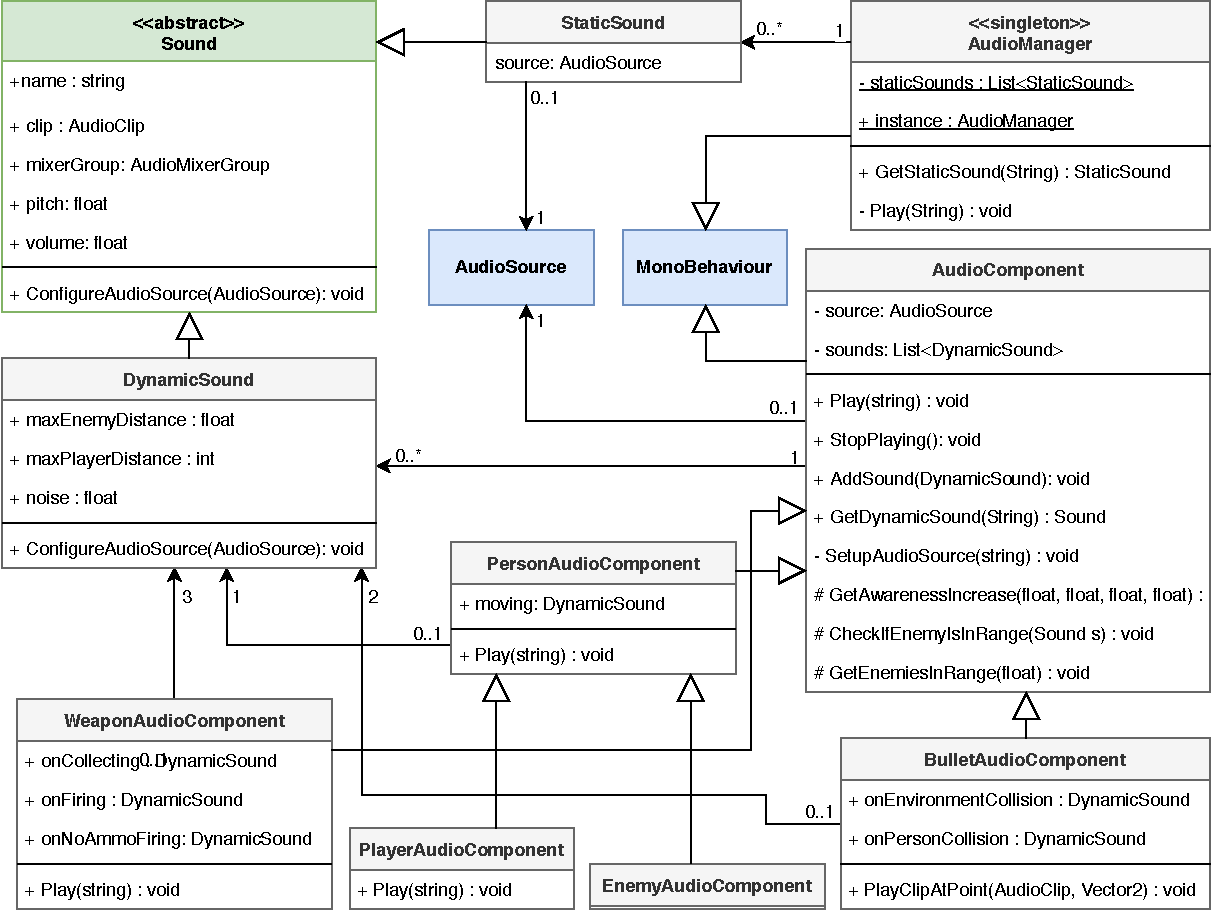
\includegraphics[width=1\textwidth]{pics/audio_audiosystem.pdf}
		\caption{Das Audio-System}
		\label{fig:audio_system}
	\end {center}
\end {figure}
Aus den vorangegangenen Überlegungen wurde das in Abbildung \ref{fig:audio_system} zu sehende Klassendiagramm für das Audiosystem entworfen und implementiert. Dabei wurden die einem \textit{Prefab} zuordnungsbaren Konfigurationsobjekte in eine eigene Komponente ausgelagert und an das Spielobjekt des \textit{Prefabs} gebunden. Dadurch entsteht keine direkte Zuordnung zwischen der Klasse und der Audiokomponente. Die Klasse muss nur auf die Basisklasse \textit{AudioComponent} zugreifen und die Methode \texttt{Play(...)} aufrufen. Durch Vererbung kann dazu diese Methode an bestimmte Typen wie Geschosse, Waffen oder Gegnern und Spielern angepasst werden. Dies ermöglicht es auch im Code nicht spezifizieren zu müssen, welche Tonspur von welcher Waffe genau abgespielt werden soll. Es reicht der Komponente mitzuteilen, dass die Tonspur zum Abfeuern der Waffe abgespielt werden soll. Dadurch sind die Abhängigkeiten im Code zur Audiokomponente geringer als bei Verwendung einer zentralen Instanz.

\subsection{Gegner reagieren auf Geräusche} \label{sec:gegnerreaktionaufaudio}
Im Spiel sollen Geräusche, die der Spieler verursacht einen Gegner auf diesen aufmerksam machen können, sodass der Gegner den Spieler gegebenenfalls sucht und bei Sichtkontakt angreift. 

\subsubsection{Designmöglichkeiten}
Es gibt grundsätzlich zwei Möglichkeiten der Umsetzung:
\begin{enumerate}
	\item Gegner prüfen in regelmäßigen Abständen auf Geräusche in der näheren Umgebung.
	\item Geräusche benachrichtigen Gegner in der näheren Umgebung.
\end{enumerate}

Der erstere Ansatz würde dazu führen, dass für den Spieler unverständliche Effekte auftreten könnten wie beispielsweise, dass die Aufmerksamkeitsanzeige eines Gegners bei einem vom Spieler verursachten sehr lauten Geräusch in seiner näheren Umgebung entweder gar nicht oder sofort stark ansteigt. Dies liegt daran, dass ein Radius um den Gegner herum bestimmen würde, ob ein Geräusch erkannt werden kann oder nicht. Wie laut das Geräusch dabei ist, spielt zunächst keine Rolle. Würde man versuchen alle möglichen Geräusche miteinzubeziehen, die die Aufmerksamkeit des Gegners erhöhen könnten, so müsste man den Radius auf das lauteste Geräusch setzen, das der Gegner hören könnte. Wird dies umgesetzt, so würden auch sehr viele leisere Geräusche zunächst dabei sein, die nach der Berechnung für die Reichweite der Lautstärke und dem Vergleich der Distanz zum Gegner wieder aussortiert werden. %Die bei dieser Variante resultierende Überlegung ist einen fließenden Übergang durch mehrere Bereiche um den Gegner herum nachzuahmen. Dieser fließende Übergang ist bei letzterer Variante bereits vorhanden: 
Diese unnötige Berechnung ist bei letzterer Variante nicht vorhanden: Dadurch, dass einem Geräusch eine Lautstärke  als Attribut gegeben werden kann, kann auch der Radius für jedes Geräusch, in dem es Gegner aufmerksam macht, flexibel eingestellt werden.   

Daneben muss unterschieden werden, ob der Spieler oder der Gegner das Geräusch verursacht hat. Dabei wurde festgelegt, dass für Waffen und Projektile egal ist, ob ein Spieler oder ein Gegner die zugehörigen Geräusche verursacht hat, da ein Gegner seine Waffe nicht einsetzen würde, wenn ein Spieler nicht in der näheren Umgebung wäre. Durch Vererbung kann bei der zweiten Variante vermieden werden, dass die Funktion für die Benachrichtigung über ein Geräusch aufgerufen wird, indem nur die Methoden \texttt{Play(...)} der Audiokomponenten von Waffen, Geschossen und Spielern diese Funktionalität aufrufen. Bei der ersteren Version muss hingegen eine Überprüfung zwingend stattfinden.

Als nächstes muss die durch diese Funktionalität  entstehende unvermeidbare Auslastung für die zusätzlichen Berechnungen berücksichtigt werden. Beim ersteren Ansatz steigt die Auslastung pro Gegner im Spiel an, da jeder Gegner andauernd prüfen muss, ob Geräusche auf einen Spieler in der Nähe Rückschlüsse ziehen lassen. Geräusche außerhalb der Aufmerksamkeitsreichweite der Gegner erhöhen hingegen nicht die Auslastung zusätzlich. Beim letzteren Ansatz verursacht potentiell jedes aktive Geräusch eine höhere Auslastung, da überprüft werden muss, ob ein Gegner in Reichweite ist. Gegner außerhalb der Reichweite der Geräuschlautstärke hingegen erhöhen die Auslastung nicht.

Die Auslastung bei beiden Varianten kann dabei auf ein Minimum reduziert werden, indem nur in einem gewissen Umkreis um den Spieler herum die zugehörigen Funktionen aufgerufen werden, wodurch beide Varianten in etwa die gleiche Auslastung verursachen sollten. Für das Spiel wurde die letztere Variante implementiert, da diese für den Spieler ein verständlicheres Verhalten von Gegnern zur Folge hat und bereits ohne größere Performanzeverbesserung gute Resultate liefert.

\subsubsection{Die Implementierung}
Für die Implementierung dieses Features kann auf das Konzept des Audiosystems zurückgegriffen werden. Dabei muss jedes mal, wenn die Methode \texttt{Play(...)} einer Audiokomponente eines Spielers, eines Geschosses oder einer Waffe aufgerufen wird überprüft werden, ob sich Gegner in der Umgebung befinden. Hierfür kann die Vererbung genutzt werden, um diese Überprüfung bei Geräuschen ausgehend von Gegnern zu vermeiden. Da jedes Geräusch eine unterschiedliche Lautstärke hat und auch die Entfernung sowie die Art des Gegners eine Rolle spielen kann, wie sehr die Aufmerksamkeit eines Gegners ansteigt, müssen diese bei der Berechnung für die Aufmerksamkeitserhöhung miteinbezogen werden. Hierfür besitzt jeder Gegner ein eigenes Attribut wie sehr die Aufmerksamkeit von diesem erhöht wird, jedes Objekt des Typs \texttt{DynamicSound} besitzt ein Attribut für die Aufmerksamkeitserhöhung und die Strecke zwischen dem Ursprungsort des Geräusches und der aktuellen Position des Gegners kann durch die zwischen diesen Positionen liegende Wegstrecke berechnet werden. Dabei wird nicht die Luftstrecke, sondern die hindernisfreie Wegstrecke des Geräusches bis zum Gegner für die Berechnung herangezogen. Für die Berechnung wird die Funktion \texttt{GetAwarenessIncrease(...)} genutzt. Dabei wird vor der Berechnung zunächst mit der Methode \texttt{GetEnemiesInRange(...)} die in der Nähe befindlichen Gegner gesucht. Sind keine Gegner in dem Wirkungsbereich des Geräusches, so wird die Methode verlassen.

\subsection{Einstellung der Lautstärke verschiedener Kategorien}
\begin {figure}[h]
	\begin {center}
	    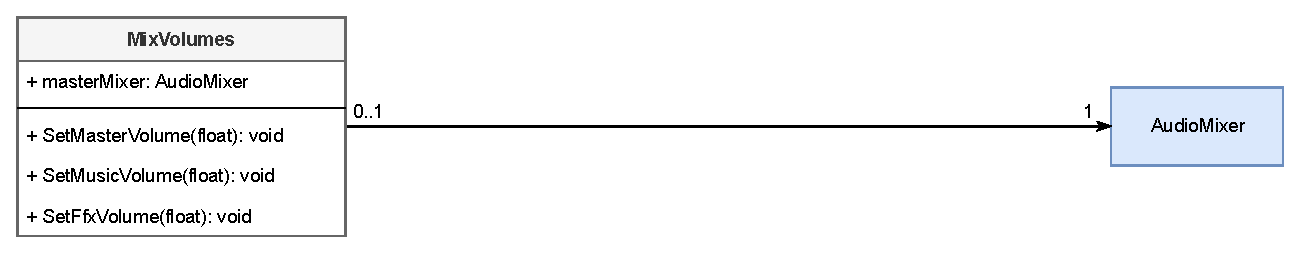
\includegraphics[width=1\textwidth]{pics/audio_category_configuration.eps}
		\caption{Implementierung für das Einstellen der Lautstärke verschiedener Kategorien}
		\label{fig:audio_category_configuration}
	\end {center}
\end {figure}
Für einen Benutzer ist es beim Audiosystem wichtig einstellen zu können, wie laut die Lautstärke jeder einzelnen Soundkategorie ist. Abbildung \ref{fig:audio_category_configuration} zeigt den hierfür implementierten Teil des Audiosystem. Aktuell kann im Optionsmenü des Hauptmenüs eingestellt werden, wie laut das Gesamtvolumen, die Hintergrundmusik und die Soundeffekte sein sollen. Das Audiosystem wurde auch in diesem Bereich so ausgelegt, dass weitere Kategorien leicht implementiert werden können. Bei jedem Schieberegler für diese Einstellungen wird bei Veränderung der Position dieses Reglers ein Event ausgelöst welches eine bestimmte Funktion in der Klasse \texttt{MixVolumes} anspricht mit dem aktuellen Stand des Reglers von null bis eins.





\pagebreak

% Serialisierung und Deserialisierung
\section{Serialisierung und Deserialisierung von Spielständen}
\label{sec:designSerialization}

In den vorhergehenden Kapiteln wurden verschiedene Funktionalitäten des Spiels ausführlich dargestellt. Wie bereits im Einführungskapitel beschrieben, soll ein Spieler die Möglichkeit haben, existierende Spielstände abspeichern sowie gesicherte Zwischenstände zu Beginn der Applikation wiederherstellen zu können. Dies geschieht über einen Serialisierungs- und Deserialisierungsprozess, der im Laufe dieses Kapitels näher erläutert wird. 

%Eine weitere Grundfunktionalität der Software stellt die Serialisierung und Deserialisierung diverser Spielszenerien dar. Ein Spieler soll die Möglichkeit haben, existierende Spielstände abspeichern sowie gesicherte Zwischenstände zu Beginn der Applikation wiederherstellen zu können. 

Im Folgenden wird zunächst die Wahl eines geeigneten Dateiformats zur Sicherung von Spiel\-stän\-den beschrieben. Anschließend werden grundlegende Designentscheidungen zur Erfüllung dieser Anforderungen erläutert. Abschließend wird der Prozess des Speicherns und Ladens eines Levels dargestellt. 

\subsection{Wahl eines geeigneten Dateiformats}


Die Sicherung eines Spielstandes erfolgt in einer hierarchisch strukturieren Textform. Hierzu existieren verschiedene Möglichkeiten, deren Vor- und Nachteile es gegeneinander abzuwägen gilt. 

Eine nahe liegende Variante stellt die \textit{Erweiterbare Auszeichnungssprache} (engl. \textit{Extensible Markup Language, XML}) dar. Die gewünschte hierarchische Struktur wird hierbei durch das Verschachteln verschiedener Elemente ineinander ermöglicht. Ein wesentlicher Vorteil dieser Notation ist, dass es sich um einen offenen Standard handelt, der vom World Wide Web Consortium (W3C) entwickelt und dort weiterhin gepflegt wird. Des Weiteren können Dateien dieses Formats von Menschen gelesen und verstanden werden. Dies begünstigt die Wartbarkeit und führt zu einer schnelleren Fehlerbehebung im Zuge des Entwicklungsprozesses. 

Die \textit{JavaScript Objektnotation} (engl. \textit{JavaScript ObjectNotation, JSON}) stellt eine weitere Möglichkeit zur Speicherung hierarchisch organisierter Daten dar. Das JSON Dateiformat verfügt über alle zuvor genannten Vorteile von XML. Darüber hinaus benötigt ein JSON Dokument aufgrund der wesentlich simpleren Syntax deutlich weniger Speicherplatz als eine vergleichbare XML Datei mit identischem Inhalt. Die geringere Dateigröße bietet einen großen Vorteil hinsichtlich der konkreten Aufgabe, da Speicher- und Wiederherstellungsprozesse performanter ausgeführt werden können. Des Weiteren können hierdurch auch umfangreichere Spielzwischenstände mit vergleichsweise geringen Dateigrößen gesichert werden. Nach Gegenüberstellung der Vor- und Nachteile beider Dateiformate wurde daher entschieden, die Spielzwischenstände im JSON Format zu sichern. 


%XML:
%- Offener Standard
%- Dateien können nicht nur von Maschinen, sondern auch von Menschen gelesen werden.
%- Erlaubt Strukturierung von Daten -> Verschachtelung möglich / Hierarchie realisierbar
%- Hinter XML steht nicht eine einzelne Firma, sondern es wurde federführend vom World Wide Web Consortium (W3C) entwickelt und wird dort auch weiterhin gepflegt. Der Standard ist offen und für jeden einsehbar.

%Json (JavaScript ObjectNotation):
%- Alles, was XML auch bietet
%- Darüber hinaus: Schlanker -> daher schneller beim speichern/laden
%- XML ist komplizierter zu parsen als Json es ist. 

%- Format! in Form von generierten JSON-Dateien! Warum Json? Kurz, übersichtlich, Speichersparend. Vergleich mit XML, Vorteile, Nachteile. 

\subsection{Beteiligte Komponenten und grundsätzlicher Aufbau}\label{sec:structureSerialization}

In Abbildung \ref{fig:serialization_diagram} ist ein UML-Klassendiagramm mit allen Komponenten dargestellt, die im Zuge des Serialisierungs- und Deserialisierungsprozesses von Relevanz sind. Um die Übersichtlichkeit zu wahren, wurde hierbei auf sämtliche Konstruktoren sowie Getter und Setter Methoden aller Klassen verzichtet. Des Weiteren wurden nur Klassen, Beziehungen, Attribute und Methoden in das Diagramm aufgenommen, die im Zuge des Serialisierungs- und Deserialisierungsprozesses aktiv genutzt werden. 

Anhand des Diagramms ist zu erkennen, dass der \texttt{LevelController} die zentrale Instanz darstellt. Der \texttt{LevelController} hält eine Referenz auf eine Instanz der Klasse \texttt{LevelData-\linebreak Collection}, welche wiederum Referenzen zu allen Objekten besitzt, die serialisiert und deserialisiert werden. Die Klasse \texttt{LevelDataCollection} agiert in diesem Kontext daher als eine Art Container für Level Elemente, Items und Gegner. Da sowohl die charakteristischen Daten (beispielsweise Gegnertyp, Patrouillenpunkte, ...) als auch die aktuelle Position eines Spielobjekts gespeichert werden, müssen zwei Referenzen für jeden Typ vorgehalten werden. Beispielsweise enthält das Attribut \texttt{enemyData} eine Liste mit Referenzen zu Objekten, die die charakteristischen Merkmale der Gegner beschreiben, wohingegen das Attribut \texttt{enemies} eine Liste mit Referenzen auf alle existierenden gegnerischen Spielobjekte mit ihren aktuellen Positionen enthält. Es werden Wände, Türen, Waffen, Gegner, Zielpositionen, Eigenschaften des Levels und Start- sowie aktuelle Position des Spielers abgespeichert. Für die verschiedenen Elemente werden die folgenden Attribute serialisiert und deserialisiert:

\vspace{3mm}
\begin{tabular}[t]{ll}
%\tabitem 
\textbf{Wand:} & Position\\
\textbf{Tür:} & Position, Rotation\\
\textbf{Waffe:} & Position, Rotation, Typ, Munitionsmenge\\
\textbf{Gegner:} & Position, Typ, Patrouillenpunkte, Waffentyp, Munitionsmenge\\
\textbf{Zielzone:} & Position\\
\textbf{Level:} & Größe\\
\textbf{Spieler:} & Aktuelle Position, Waffentyp, Munitionsmenge
\end{tabular}
\vspace{4mm}


Des Weiteren besitzt der \texttt{LevelController} Beziehungen zu allen Klassen, die an der logischen Umsetzung des Serialisierungs-/Deserialisierungsprozesses beteiligt sind. Klassen, die die Schnittstelle \texttt{ILevelDataProvider} implementieren, verfügen über Methoden, die Informationen bezüglich der verschiedenen Spielelemente liefern und agieren somit als Datenquelle. In Abbildung \ref{fig:serialization_diagram} wird die Methode \texttt{GetEnemyData()} stellvertretend für alle Methoden der verschiedenen Spielelemente dargestellt. Die Schnittstelle \texttt{ILevelLoader} implementierende Klassen sind für die Instanziierung der konkreten Spielobjekte verantwortlich, ausgehend von den Informationen eines konkreten \texttt{ILevelDataProviders}. Die Methoden \texttt{SerializeLevel(...)} und \texttt{DeserializeLevel(...)} der Schnittstellen \texttt{ILevelSerializer} und \texttt{ILevelDeserializer} implementieren die entsprechende Logik für den jeweiligen Vorgang. Um das Ersetzbarkeitsprinzip (auch Liskovsches Substitutionsprinzip genannt, siehe \cite{Liskov_Substitution_Principle}) zu erfüllen, werden als Datentyp dieser vier Variablen innerhalb des \texttt{LevelControllers} ausschließlich die jeweiligen Schnittstellen-Typen verwendet. Zur Laufzeit werden diese Typen durch konkrete, die Schnittstelle implementierende Klassen ersetzt. 

%\vspace{1em}
%\begin{minipage}{\linewidth}
\begin{figure}
	\centering
	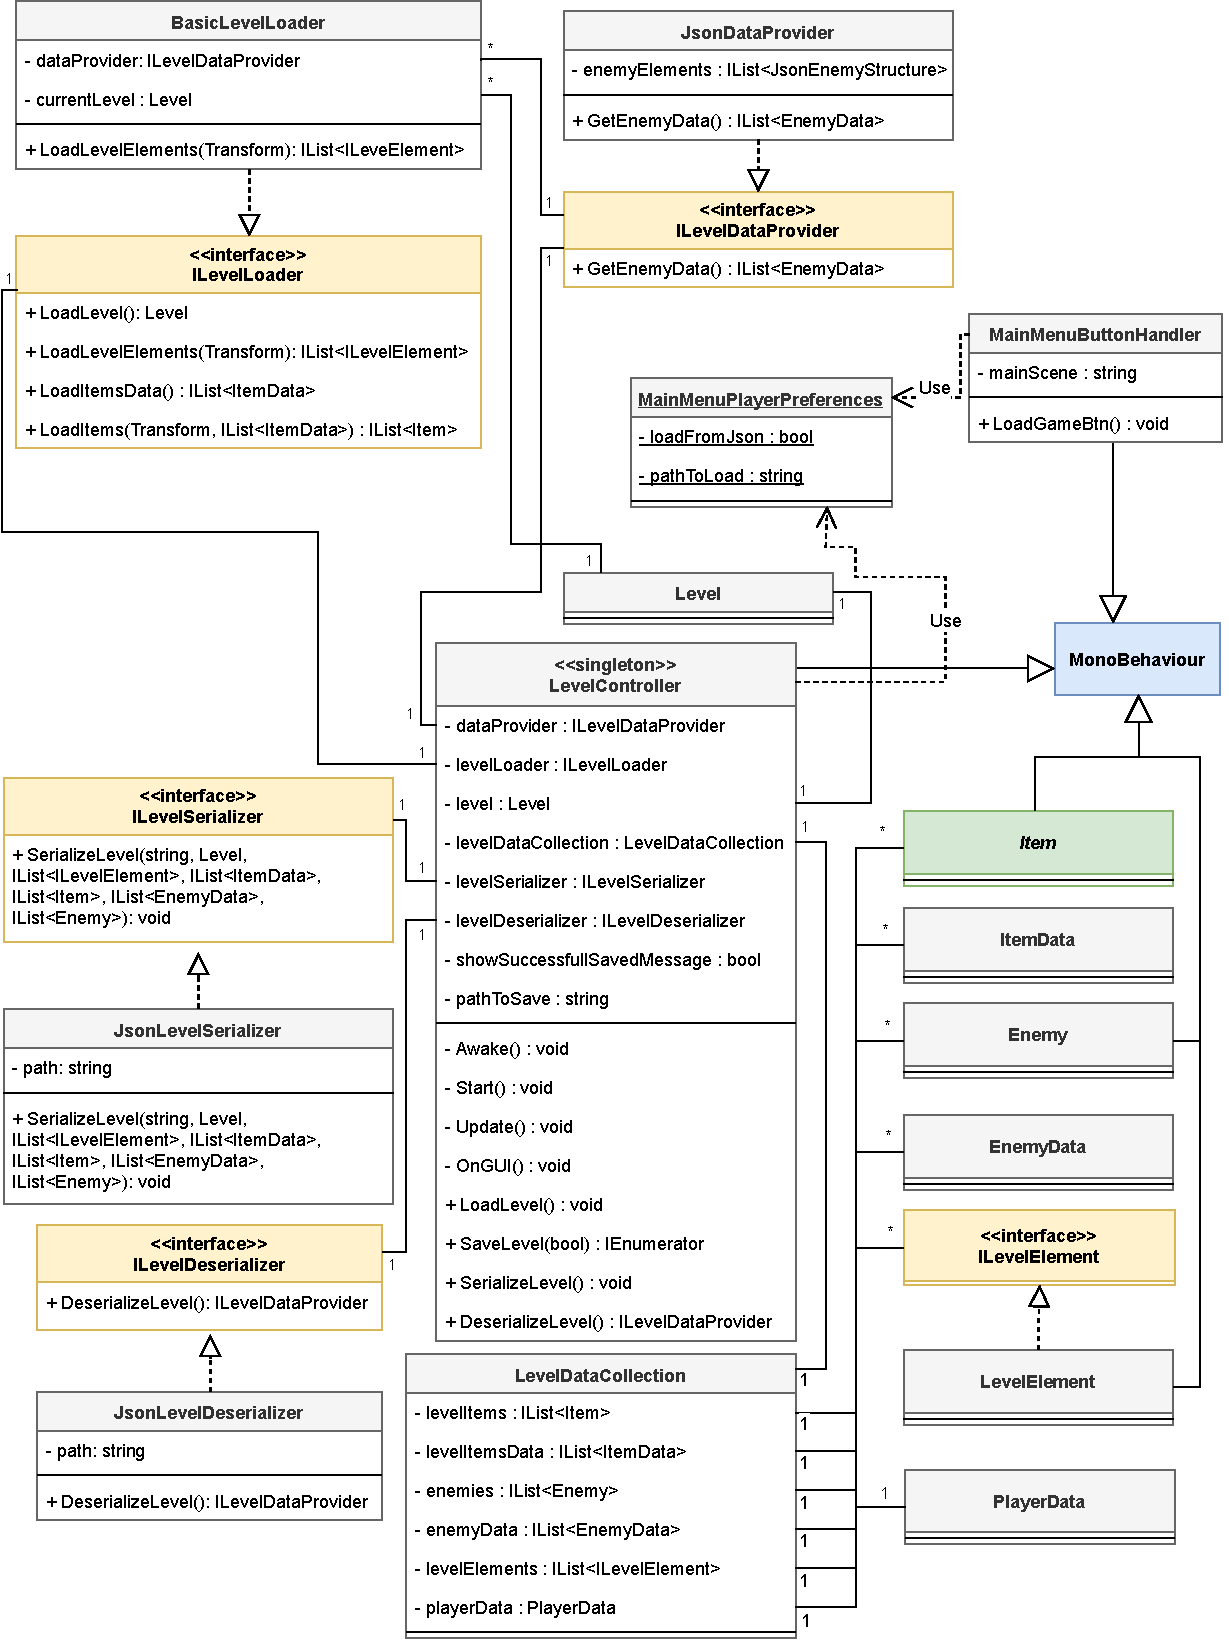
\includegraphics[width=1.00\linewidth]{diagrams/Level_Serialization_Deserialization_reduced.pdf}
	\captionof{figure}[Komponenten der Serialisierung und Deserialisierung]{UML-Klassendiagramm aller am Serialisierung- und Deserialisierungsprozess beteiligten Komponenten.}
	\label{fig:serialization_diagram}
	\end{figure}
%\end{minipage}

%- Im UML zu sehen, stark gekürzt.
%- Was wird serialisiert/deserialisiert? Welche Attribute? Sieht man im UML gekürzt. 
%- LevelController hält alles (Referenzen auf alles zu ser. des. bare)
%- Referenzen auf ILevelSer. und ILevelDes.
%- Ref. auf ILeveDataProvider, stellt die Daten für die Spielobjekte bereit. Im UML wurde exemplarisch nur für Enemies die Methode gezeigt. es existieren natürlich mehr. 
%- Referenzen auf ILevelLoader, erstellt konkrete Spielobjekte
%- Interfaces, um erweiterbar. => Liskovsches Substitutionsprinzip oder auch Ersetzbarkeitsprinzip. Interface Typen können durch konkrete abgeleitete Klassen ersetzt werden. 

%- Im UML:
%=> Verzichten auf Konstruktoren, Getter und Setter.

\subsection{Speichern eines Spielstands}
%
%Der Ablauf zum Speichern eines Spielstandes beginnt, sobald im laufenden Spiel die F2 Taste betätigt wird. Das Eintreten dieser Aktion wird in der \texttt{Update()} Methode des \texttt{LevelControl-\linebreak lers} zyklisch überprüft.

Der Ablauf zum Speichern eines Spielstandes beginnt, sobald im laufenden Spiel die "`F2"' oder "`F3"' Taste betätigt wird. Das Eintreten einer dieser Aktionen wird in der \texttt{Update()} Methode des \texttt{LevelControllers} zyklisch überprüft. Sobald eines dieser beiden Ereignisse eintritt, wird die Koroutine \texttt{SaveLevel(bool selectPath)} aufgerufen. Der Parameter \texttt{selectPath} hängt von der betätigten Taste ab und indiziert, ob der Benutzer den Standardpfad zur Sicherung der JSON Datei anpassen möchte. 

Durch Betätigung der "`F2"' Taste signalisiert ein Spieler der Unity-Engine, dass er den Pfad, an dem die zu sichernde JSON Datei abgelegt werden soll, selbst spezifizieren möchte. Hierzu wird der \texttt{SaveLevel(...)}-Koroutine der boolsche Wert \texttt{true} als Argument übergeben. Es öffnet sich daraufhin ein Dialog, der den Benutzer auffordert, einen Speicherort für die zu sichernde JSON Datei zu selektieren. Der Dateiname setzt sich standardmäßig aus einem fixen Präfix gefolgt vom aktuellen Datum und der momentanen Uhrzeit zusammen. 

Sollte die Aktion durch das Betätigen der "`F3"' Taste ausgelöst worden sein, öffnet sich kein Dialog und das Präfix des Dateinamens deutet auf eine Schnellspeicherung hin. In diesem Fall wird der boolsche Indikator \texttt{showSuccessfulSavedMessage} innerhalb der \texttt{SaveLevel(...)}-Methode auf \texttt{true} gesetzt. Innerhalb der von \textit{MonoBehaviour} geerbten Methode \texttt{void OnGUI()} wird dieser Wert einmal pro Einzelbild abgefragt. Solange dieser \texttt{true} ist, wird dem Spieler eine Meldung auf dem Bildschirm angezeigt, die über den Erfolg des Speichervorgangs Rückmeldung gibt. Nach einer festgelegten Zeitspanne von drei Sekunden wird das Attribut \texttt{showSuccessfulSavedMessage} wieder auf den Wert \texttt{false} gesetzt, und die Benachrichtigung verschwindet wieder.

Sobald der Dateiname für die zu sichernde Datei feststeht, wird im \texttt{LevelController} die Methode \texttt{SerializeLevel()} aufgerufen. Im Falle einer Schnellspeicherung geschieht dies noch vor der Rückmeldung des Speichererfolgs an den Benutzer. Innerhalb dieser Methode wird ein konkreter \texttt{JsonLevelSerializer} instanziiert und dessen \texttt{SerializeLevel(...)}-Methode mit allen Argumenten aufgerufen, die für den Serialisierungsprozess von Relevanz sind. 

Die konkrete Logik zur Serialisierung erfolgt anschließend in dieser Methode. Die benötigten Daten der übergebenen Argumente werden in hierfür speziell vorgesehene Klassen überführt, die ausschließlich zu Serialisierungszwecken instanziiert werden und nur die notwendigen Attribute beinhalten. Die gewünschte hierarchische Struktur innerhalb der zu generierenden JSON Datei wird durch Referenzen innerhalb dieser Klassen untereinander realisiert. Auf Basis dieser Dateien wird im Anschluss mithilfe des Frameworks Json.NET\footnote{https://www.newtonsoft.com/json} eine entsprechende JSON Datei generiert. Abschließend wird diese Datei am Ort des gewählten Pfades im Dateisystem abgelegt. 

%- Szene ist geladen. In der Update vom LevelController auf F2 lauschen. File Dialog öffnen.
%- Standardtext im File Dialog.
%- Rufe SerializeLevel vom LevelController auf
%- Instanziiere konkreten JsonLevelSerializer
%- Rufe Methode von JsonLS auf und übergebe alles relevante (was wird übergeben, siehe JSON)
%- Informationen aus Data und konkreten Spiel Objekten werden in Json Klassen überführt
%- Benutzte Framework -> einfach zu benutzen -> spart Performanz im Gegensatz zu selber schreiben
%- Schreibe Json File ins FileSystem.

\subsection{Laden eines Spielstands}

Beim Starten der Applikation kann ein existierender Spielstand geladen werden. Hierzu muss der Spieler im Hauptmenü die entsprechende Schaltfläche betätigen. Es öffnet sich dann ein Dialog, der den Benutzer auffordert, die wiederherzustellende JSON Datei zu selektieren.

Das Hauptmenü existiert in einer eigenen Szene, unabhängig von der eigentlichen Spielszene. Dies bedeutet, dass zentrale Komponenten, wie beispielsweise der \texttt{LevelController}, zu diesem Zeitpunkt noch nicht existieren und erst mit dem Wechsel zur Hauptszene geladen werden. Es ist lediglich die Klasse \texttt{ButtonHandler} vorhanden, in der die Wahl des Benutzers (neues Spiel beginnen oder existierenden Spielstand laden) in Form einer boolschen Variable sowie gegebenenfalls der Pfad zur wiederherzustellenden Datei gespeichert sind. Entscheidet sich der Spieler dazu, einen existierenden Spielstand zu laden, wird dieser Indikator auf \texttt{true} sowie der entsprechende Pfad gesetzt.

Im Anschluss wird die Hauptszenerie mit all ihren Komponenten erstellt. Die Logik des \texttt{Level-\linebreak Controllers} hängt dabei allerdings von den Eingaben des Benutzers ab. Dazu müssen die im \texttt{ButtonHandler} vorhandenen Informationen in irgendeiner Weise über die beiden Szenen hinweg an den \texttt{LevelController} übertragen werden. Hierfür sind verschiedene Möglichkeiten denkbar, die jeweils mit Vor- und Nachteilen verbunden sind.

\subsubsection{Übertragen von Informationen über mehrere Szenen hinweg}

Eine simple Möglichkeit zur Übertragung von Informationen über mehrere Szenen hinweg stellt die Verwendung von \textit{PlayerPrefs} \cite{Unity_Doc_PlayerPrefs} dar. Dabei handelt es sich um einen von Unity bereitgestellten Mechanismus, der es dem Entwickler ermöglicht, verschiedene Informationen im Dateisystem zu sichern und zu einem späteren Zeitpunkt wieder abzufragen. Die Verwendung ist aufgrund der von Unity bereitgestellten Funktionalität äußerst simpel. Des Weiteren ermöglicht dieses Vorgehen eine Sicherung von Informationen über mehrere Anwendungen hinweg, da die gespeicherten Daten mit Spielende nicht automatisch gelöscht werden. Die direkte Speicherung von Informationen auf Ebene des Dateisystems ist allerdings auch mit negativen Aspekten verbunden. Da die zu sichernden Daten beispielsweise im Falle eines Windows-Betriebssystems direkt in der Registrierungsdatenbank festgeschrieben werden, skaliert das Vorgehen sehr schlecht für Applikationen, in denen viele Daten vorgehalten werden müssen. Zudem werden die Einträge in der Registrierungsdatenbank unverschlüsselt und ohne jeglichen Sicherheitsmechanismus abgelegt, wodurch gespeicherte Informationen jederzeit durch Unbefugte eingesehen und manipuliert werden können. 

Ein ähnlicher Ansatz wie der soeben beschriebene ist, die Speicherung der zu übertragenden Informationen selbst zu implementieren. Hierdurch kann der Speicherort des zu sichernden Dokuments frei gewählt sowie potenzielle Verschlüsselungsmechanismen zum Schutz der Datenintegrität verwendet werden. Der lesende und schreibende Zugriff auf diese Datei ist allerdings mit nicht unerheblichem zeitlichem Aufwand verbunden, der abhängig von der jeweiligen Verschlüsselungstechnologie weiter ansteigen kann.

Als Alternative zu den beiden obigen, dateibasierten Ansätzen, ist die Verwendung einer Singleton Klasse eine weitere Möglichkeit zur Übertragung von Informationen über verschiedene Szenen hinweg. Dabei wird beim ersten Aufruf der \texttt{Instance()}-Methode eine neue Instanz der jeweiligen Klasse erzeugt und einer statischen \texttt{instance} Variablen zugewiesen, die auch nach einem Wechsel der Spielszene weiterhin existiert. Bei allen weiteren Aufrufen dieser Methode wird die Referenz auf die instanziierte Klasse zurückgegeben. Hierdurch entfällt die Verwaltung eines externen Dokuments und alle relevanten Daten werden innerhalb der Applikation vorgehalten. Dies bietet zum einen zeitliche Vorteile bei schreibenden und lesenden Zugriffen auf die Daten, zum anderen muss keine extra Datei im Dateisystem abgelegt werden. 
%Im konkreten Fall ist die Verwendung der \texttt{MainMenuButtonHandler} Klasse als Singleton allerdings nicht ohne Weiteres möglich, da diese Klasse von \texttt{MonoBehaviour} erbt und somit nicht instanziiert werden kann. 

Eine zentrale Datenhaltung mit globalem Zugriff innerhalb der gesamten Applikation kann auch in Form einer statischen Klasse realisiert werden. Diese bietet alle oben genannten Vorteile des Singleton Entwurfsmusters und lässt sich des Weiteren äußerst einfach realisieren. Im Gegensatz zu Singleton Klassen können statische Klassen nicht als Parameter in Methoden übergeben werden, können keine Schnittstellen implementieren und nicht von anderen Klassen erben. Da im konkreten Fall keine dieser Techniken verwendet wird, existiert kein Grund, der gegen die Verwendung einer statischen Klasse spricht. Es existiert daher eine statische Komponenten mit dem Namen \texttt{MainMenuPlayerPreferences}, deren Eigenschaften durch die Klasse \texttt{MainMenuButtonHandler} gesetzt werden und im \texttt{LevelController} zu einem späteren Zeitpunkt ausgelesen werden. 



%https://gamedev.stackexchange.com/questions/110958/what-is-the-proper-way-to-handle-data-between-scenes
%
%=> Bei DestroyOnLoad wird das GameObject die ganze Zeit über vorgehalten (=> also das MonoBehaviour), bei static class nur die Klasse!

\subsubsection{Erstellen der Spielobjekte}

Der \texttt{LevelController} ruft in seiner \texttt{Start()}-Methode beim Laden der Hauptszene den boolschen Indikator \texttt{LoadFromJson} der statischen Klasse \texttt{MainMenuPlayerPreferences} ab. Anhand dieses Indikators entscheidet der \texttt{LevelController}, welcher \texttt{ILevelDataProvider} als Quelle zur Instanziierung der Spielobjekte verwendet wird. Sollte die Variable \texttt{false} sein, wird die Klasse \texttt{TestLevelDataProvider} instanziiert. Diese stellt ein vordefiniertes Standardlevel mit verschiedenen Level Elementen, Items und Gegnern zur Verfügung. Andernfalls wird die private Methode \texttt{DeserializeLevel()} aufgerufen und deren Rückgabewert verwendet.

Innerhalb der privaten Methode \texttt{DeserializeLevel()} wird eine neue Instanz der Klasse \texttt{Json-\linebreak LevelDeserializer} mit dem Pfad der entsprechenden JSON Datei instanziiert. Dieser Pfad wird aus der statischen Komponente \texttt{MainMenuPlayerPreferences} ausgelesen. Durch einen Aufruf der Methode \texttt{DeserializeLevel()} der Klasse \texttt{JsonLevelDeserializer} erfolgt die Umkehroperation der Serialisierung: Das selektierte JSON Dokument wird mithilfe des Json.NET Frameworks in die jeweiligen JSON-Klassen konvertiert und es wird ein \texttt{JsonDataProvider} zurückgegeben.

Dieser wird anschließend im \texttt{LevelController} als Datenquelle zur Erstellung der Spielobjekte genutzt. Hierzu wird ein \texttt{BasicLevelLoader} mit dem soeben erzeugten Objekt als Konstruktorargument instanziiert. Dieser erzeugt durch die Verwendung diverser statischer Fabrikmethoden der Klassen \texttt{LevelElementFactory} und \texttt{ItemFactory} konkrete Spielobjekte aus den Daten des übergebenen \texttt{JsonDataProviders}. Die Erstellung der Spielobjekte für die Gegner und den Spieler erfolgt anschließend innerhalb der \texttt{LoadEnemies(...)} und \texttt{StartLevel()}-Methode im \texttt{LevelController} durch die Verwendung entsprechender statischer Fabrikmethoden der Klasse \texttt{PersonController} auf Basis des vorhandenen \texttt{JsonDataProviders}.
%Dieser erzeugt durch die Verwendung diverser Fabrikmethoden konkrete Spielobjekte aus den Daten des übergebenen \texttt{JsonDataProviders}.





%- Starten der Applikation kann Spielstand geladen werden. Menü existiert in seperater Szene.
%- Starten der App. -> Menü Szene öffnet sich -> ButtonHandler Klasse ist instanziiert
%- Klick auf "Load Game" öffnet File Dialog , selektiere Pfad zum Laden
%- Das Bool Flag LoadGame und der Pfad müssen zwischen den Szenen übergeben werden (LevelController existiert noch nicht). Dafür gibt es unterschiedliche Möglichkeiten:
%	=> PlayerPrefs
%	...
%	=> Vorteile/Nachteile aufzeigen!
%- Laden der MainScene -> LevelController -> In der Awake wird das Flag geprüft und ggf. der Pfad gesetzt
%- In der Start (also Erstellung der Szene) wird geprüft, ob Flag true ist. Wenn nein => wähle Standard Data Provider, wenn ja => rufe LevelController Methode DeserializeLevel auf. Dort instanzieere Klasse, rufe Methode auf, returned ILevelDataProvider. Nutze dann diesen. 
%- BasicLevelLoader Instanz erstellen. ABhängig vom ILevelDAtaProvider erstellt dieser die konkreten Spielobjekte in der Szene. 



%\textbf{TODO} UML Diagramme für den Ser./Des. Prozess hier einfügen. Kurz auf die geplanten Features eingehen (Level speichern, Laden eines Levels, Laden eines vorhandenen Spielstandes).



%\textbf{TODO} Json-Listing hier einfügen. Unterkapitel machen: Ablauf beim Level speichern und laden erläutern. Json-File erklären. 

%%\vspace{25px}
%\begin{figure}[!t]
%\begin{lstlisting}[language=json,firstnumber=1,caption={Todo},captionpos=b,label={point_visualization}]
%{
%	"Size": {
%		"x": 64,
%		"y": 64
%	},
%	"SpawnPosition": {
%		"x": 3.0,
%		"y": 3.0
%	},
%	"ActualPosition": {
%		"x": 5.77,
%		"y": 5.44
%	},
%	"LevelElements": {
%		"Walls": [{
%				"Position": {
%					"x": 2,
%					"y": 0
%				}
%			}],
%		"Doors": [{
%				"Position": {
%					"x": 38,
%					"y": 11
%				},
%				"Rotation": "HORIZONTAL" 
%			}] 
%	},
%	"LevelItems": {
%		"Weapons": [{
%                "Position": {
%                    "x": 3.5,
%                    "y": 6.0
%                },
%                "Rotation": 30.0,
%                "Type": "PISTOL",
%                "Amount": 12
%            }]
%	},
%	"Enemies": [{
%            "Position": {
%                "x": 5.33,
%                "y": 61.5
%            },
%            "Type": "BASIC",
%            "PatrolPoints": [{
%                    "x": 14.0,
%                    "y": 61.0
%                },
%                {
%                    "x": 2.0,
%                    "y": 61.0
%                }],
%            "WeaponType": "MACHINEGUN",
%            "Amount": 20
%        }]
%}
%\end{lstlisting}
%\end{figure}
\pagebreak

% Schnittstelle für Machine-Learning
\section{Design und Implementierung einer Schnittstelle für maschinelles Lernen}\label{sec:aiInterface}

Wie im Einführungskapitel beschrieben ist es ein Ziel des Projektes, eine Grundlage für ein weiteres Projekt mit dem Thema \textit{maschinelles Lernen} (engl. \textit{machine learning}) zu schaffen. Dazu wird eine Schnittstelle benötigt, über die mithilfe der im vorherigen Kapitel beschriebenen Serialisierung und Deserialisierung Informationen über den Spielstand übertragen und Teile des Spiels gesteuert werden können.

\subsection{Umfang der Schnittstelle}\label{sec:interfaceDesign}

Die Schnittstelle umfasst eine Steuerung und Ausgabe relevanter Informationen für die Nicht-Spieler-Charaktere, mit dem Ziel, eine Verbesserung der Benutzererfahrung durch maschinelles Lernen zu ermöglichen. Dabei wäre es beispielsweise denkbar, dass sich die Schwierigkeit der Gegner an die Spielweise des Nutzers anpasst.

Gesteuert werden die Bewegungen der Charaktere inklusive Blickrichtung und Geschwindigkeit, die Attacken mit und ohne Waffe sowie die Interaktionen mit Gegenständen in der Umgebung. Außerdem ermöglicht die Schnittstelle einen Abbruch der Steuerung, die bewirkt, dass der Gegner zu seinem Standardverhalten zurückkehrt (siehe \ref{sec:enemyDesign}).

Zu den relevanten Informationen, die übergeben werden, gehören Informationen über den gesteuerten Charakter. Diese umfassen die am Prefab eingestellten Werte für den Charaktertyp, zum Beispiel die maximale Geschwindigkeit oder die Größe des Sichtfeldets, sowie charakterspezifische Eigenschaften wie die Waffe und die Menge an Munition. Ebenso wichtig sind Informationen über den Status des Charakters, darunter die verbleibende Anzahl an Leben sowie die aktuelle Position und Geschwindigkeit. Außerdem werden Informationen über das Level benötigt, insbesondere über die Objekte in der Umgebung sowie durch den Spieler verursachte Geräusche. Die Informationen über den Aufbau des Levels und die Spieler-Position werden dabei bewusst auf die direkte Umgebung des Charakters eingeschränkt, um die Entwicklung eines allwissenden Gegners zu verhindern.

\subsection{Vernetzung}\label{sec:interfaceSocket}

Eine Möglichkeit für die Erzeugung einer Schnittstelle zu einem anderen Programm ist der Unity-eigene Networkmanager \textit{UNet} \cite{Unity_Doc_UNet}, mit dem sehr leicht Verbindungen zu anderen Programmen hergestellt werden können. \textit{UNet} ist sehr mächtig, allerdings wird die Unterstützung in absehbarer Zeit eingestellt werden, da ein neues System entwickelt wird. Zudem wurde \textit{UNet} explizit für die Entwicklung von Multiplayer-Spielen entwickelt, weshalb der potenzielle Nutzer der Schnittstelle für seine Applikation ebenfalls an Unity gebunden wäre.

Da eine flexible, platformunabhängigen Schnittstelle erstrebenswert ist, sind \textit{TCP Sockets} die bessere Wahl \cite{Microsoft_Socket}. Dazu wird zu der Hauptszene des Spiels ein Controller hinzugefügt, der für die Schnittstelle zuständig ist. Dieser Controller hat eine Komponente namens \texttt{Socket-\linebreak Component}, die für die Herstellung der Verbindung sowie die Datenübertragung zuständig ist. Empfangene Daten werden für die Weiterverarbeitung an die ebenfalls am Controller hängende AIInterfaceComponent weitergegeben (siehe \ref{sec:interfaceControls}). Außerdem werden in einem festen Zeitabstand die Umgebungsdaten der aktiven Gegner an alle Clients übertragen (siehe \ref{sec:interfaceSerialization}).

Am Controller kann im Unity-Editor über die öffentlichen Variablen der Socket-Komponente der Zeitintervall für die Übertragung der Daten eingestellt werden sowie ob und an welchem Port eine Verbindung hergestellt werden soll.

\subsection{Steuerung eines Charakters}\label{sec:interfaceControls}

Um einen Charakter zu steuern, muss über die TCP-Verbindung ein Befehl im JSON-Format an das Unity-Spiel gesendet werden. Die Befehlsstruktur ist in der Klasse \texttt{JsonEnemyCommand- \linebreak Structure} definiert. Der Befehl enthält die ID des zu steuernden Charakters und den Namen des auszuführenden Befehls sowie gegebenenfalls notwendige Zusatzinformationen.

Empfangene Befehle werden durch die Socket-Komponente an die \texttt{AIInterface}-Komponente weitergeleitet, wo sie deserialisiert werden. Mithilfe des \texttt{PersonControllers} wird anhand der ID der richtige Gegner ermittelt und die entsprechende Methode der Schnittstellenkomponente des Gegners ausgeführt. Das Standardverhalten des Gegners wird daraufhin abgebrochen und es werden nur noch die Befehle ausgeführt, die von dem Socket empfangen werden.

Die Schnittstellenkomponente des Gegners hat folgende Methoden:

\begin{itemize}
	\item \texttt{SetDestination(Vector2 destination, float velocity)}
	\item \texttt{SetRotation(float rotation)}
	\item \texttt{FireWeapon()}
	\item \texttt{DropWeapon()}
	\item \texttt{CloseCombatAttack()}
	\item \texttt{StopOverride()}
	\item \texttt{Interact(string id)}
\end{itemize}

Mit der Methode \texttt{SetDestination(...)} kann ein neues Ziel festgelegt werden. Als Parameter werden die Zielkoordinaten sowie die Geschwindigkeit, mit der sich der Charakter bewegen soll, übergeben. Das Pfadfindung wird dabei von dem \texttt{NavAgent} des Charakters übernommen (siehe \ref{sec:pathfinding}). Über die Methode \texttt{SetRotation(...)} kann außerdem die Blickrichtung geändert werden.

Für die Attacken können die Methoden \texttt{FireWeapon()} und \texttt{CloseCombatAttack()} verwendet werden, mit \texttt{Interact(...)} und \texttt{DropWeapon()} können Waffen aufgenommen und abgelegt werden. Mit \texttt{StopOverride()} kann außerdem die externe Kontrolle des Gegners abgebrochen werden. Der Gegner kehrt daraufhin zu seinem Standardverhalten zurück.

Die IDs der aktiven Gegner sowie der interaktiven Objekte werden beim Start des Spiels generiert und können den Umgebungsdaten entnommen werden. Die ausführbaren Befehle heißen so wie die Methoden der Schnittstellenkomponente des Gegners. Ein Befehl könnte also beispielsweise so aussehen:

\texttt{
\string{
\string"EnemyID": "16a04a3a-57e2-453a-a132-3bc1543153a2",
"Method": \newline\string"SetDestination",
"Destination": \string{
"x": 12,
"y": 14
\string},
"Velocity": 3
\string}
}

\subsection{Serialisierung der Umgebungsdaten}\label{sec:interfaceSerialization}

Wie bereits beschrieben werden die für die aktiven Gegner relevanten Informationen regelmäßig über das Socket versendet. Um sicherzustellen, dass die Schnittstelle genau die Daten übergibt, die für den Gegner relevant sind, ohne dass dieser allwissend sein kann, müssen die Attribute des Gegners sowie alle Objekte im Sichtfeld des Gegners (siehe Kapitel \ref{sec:enemyImplementationAwareness}) serialisiert werden. 

Das bedeutet jedoch, dass der bestehende Level-Serializer (siehe \ref{sec:designSerialization}) hier nicht verwendet werden kann, da dieser explizit zum Serialisieren ganzer Levels entwickelt wurde. Hinzu kommt, dass hier Objekte serialisiert werden müssen, die zum Speichern des Levels nicht benötigt werden und dass bei den zu serialisierenden Objekten andere Attribute relevant sind. Außerdem kann zwischen den Objekten im Sichtfeld des Gegners und den Data-Objekten des Level-Controllers keine Verbindung hergestellt werden, sodass diese für die Serialisierung nicht verwendet werden können.

Deshalb werden eine eigene Klasse für die Serialisierung der für die Schnittstelle relevanten Daten und eigene Strukturen für die Serialisierten Objekte entwickelt.

In einem nächsten Schritt könnten die Serialisierungssysteme für das Level und für die Umgebungsdaten konsolidiert werden. Dies könnte beispielsweise mithilfe von \textit{Reflection} umgesetzt werden (siehe \cite{Reflection}).

\subsection{Implementierung einer Webapplikation}\label{sec:interfaceExample}

Zur Demonstration der Schnittstelle wird eine kleine Webapplikation geschrieben. Das Backend ist in \textit{NodeJS} geschrieben und stellt eine Verbindung zum TCP-Socket des Unity-Spiels her. Das Frontend ist mit \textit{VueJS} umgesetzt und wird im Sekundentakt aktualisiert. Die Verbindung zwischen Frontend und Backend ist mit \textit{axios} implementiert, das \textit{Routing} funktioniert mit \textit{Express}.

Im Frontend werden zur besseren Übersicht nicht alle Daten ausgegeben, sondern nur, wie in Abbildung \ref{fig:webapp} zu sehen ist, der Gegnertyp, die verbleibenden Leben, der Waffentyp und die Menge an Munition sowie die aktuelle Position und Blickrichtung. Für die verfügbaren Aktionen gibt es Schaltflächen.

\begin{figure}[h]
 \centering
 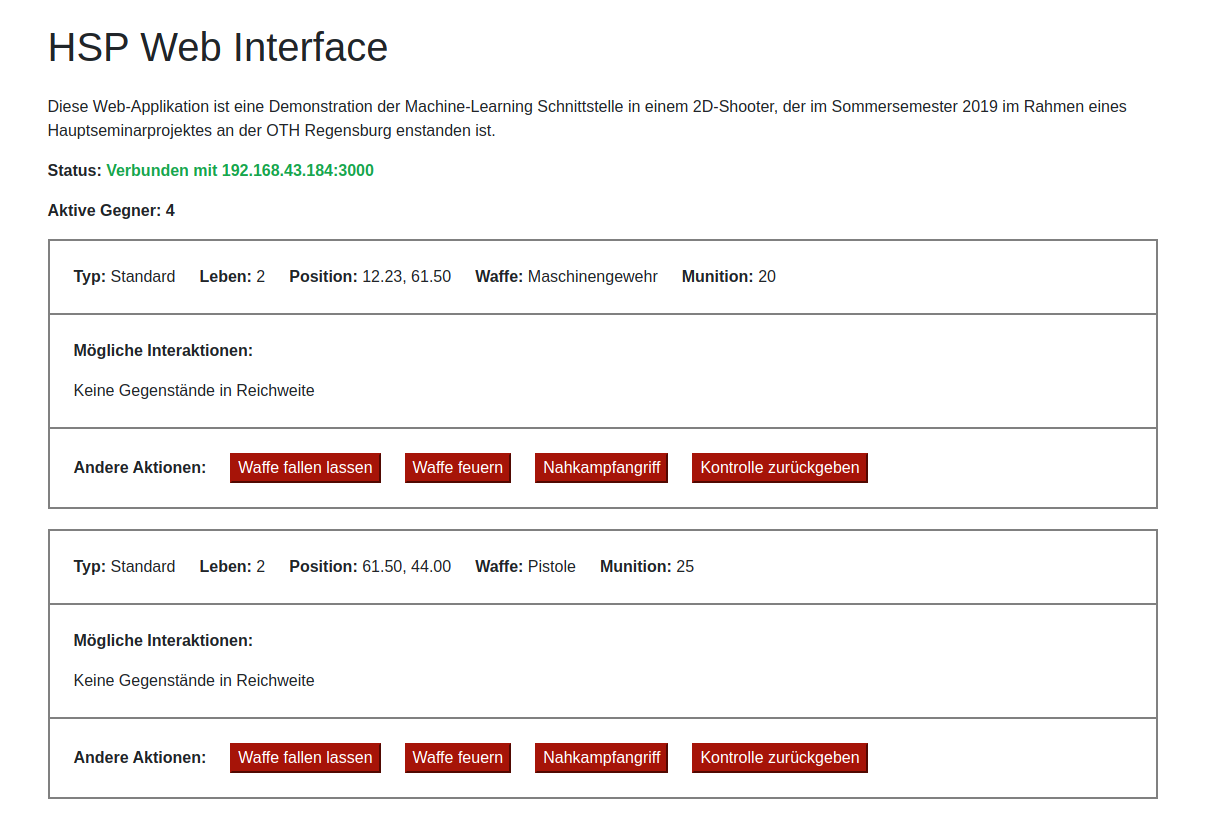
\includegraphics[width=0.835\linewidth]{pics/web-app_connected.png}
 \captionof{figure}[Demo-Applikation]{Benutzeroberfläche der Demo-Applikation}
	\label{fig:webapp}
\end{figure}

Die Applikation demonstriert nicht nur die Funktionsfähigkeit der Schnittstelle, sondern auch, dass die Programmiersprache bei der Entwicklung einer künstlichen Intelligenz zur Steuerung der Gegner keine Rolle spielt.

\subsection{Möglichkeiten der Schnittstelle}\label{sec:interfacePossibilities}

Die Schnittstelle bietet nicht nur eine Grundlage für die Forschung mit maschinellem Lernen, sondern könnte leicht erweitert werden. Es würde sich beispielsweise anbieten, die \texttt{Person} Hierarchie und die Schnittstelle so anzupassen, dass nicht nur Gegner gesteuert werden können, sondern auch der Spieler. Dies könnte auch für eine Analyse von Spielerverhalten interessant sein.

In jedem Fall sollte die Fehlerbehandlung der Schnittstelle verbessert werden, insbesondere der Umgang mit falschem Input sowie mit Verbindungsproblemen. Außerdem wäre es sinnvoll, die Optionen für die Verbindung in das Hauptmenü aufzunehmen.

\pagebreak

% Der Level Editor
\section{Der Level-Editor} \label{leveleditor}
Die Erstellung eines Levels ist in jedem Spiel sehr von Bedeutung. Dieses kann in Unity erstellt werden, indem programmiertechnisch in Skripten \textit{Prefabs} manuell instanziiert werden. Die Aufgabe der Erstellung von vielen verschiedenen Leveln wird in Unternehmen allerdings oftmals an Personen ohne tiefgreifende Kenntnisse in der Informatik weitergegeben und würde auf diese Weise zu viel Zeit in Anspruch nehmen. Um dem Spieler möglichst viel Inhalt mit möglichst geringem Entwicklungsaufwand bieten zu können, muss es möglich sein verschiedene Level leicht zu implementieren und diese testen zu können. Hierfür wird entweder ein Level-Editor oder ein Level-Generator benötigt. Das Erstellen eines Levels soll auch für Benutzer ohne Informatik-Kenntnisse geeignet sein, da diese es oft sind, die durch das Erstellen und Hinzufügen von weiteren Leveln das Interesse an diesem Spiel für die Gemeinschaft der Spieler bewahren. Um dies zu ermöglichen, wird ein Level-Editor mit grafischer Benutzeroberfläche benötigt. Im Folgenden werden Möglichkeiten zum Design eines Level-Editors untersucht. 

\subsection{Designmöglichkeiten}
Für Unity gibt es viele Tutorials, die zeigen wie man einen Level-Editor erstellt. Dabei wird meist eine sehr einfache Variante vorgestellt. Hierbei wird mit Hilfe einer Bildbearbeitungssoftware zunächst eine Karte mit Verwendung von unterschiedlichen Farben und transparentem Hintergrund erstellt wie Bild \ref{leveleditor_designarts_levelcreation} zeigt. Im Anschluss wird dieses Bild in Unity geladen und jeder farbige Pixel als ein bestimmtes Objekt interpretiert wie in Bild \ref{leveleditor_designarts_gameplay} dargestellt.

\begin{figure}[h]
    \begin{minipage}[t]{0.49\textwidth}
         \subfloat[Die Levelerstellung]{ \label{leveleditor_designarts_levelcreation}
        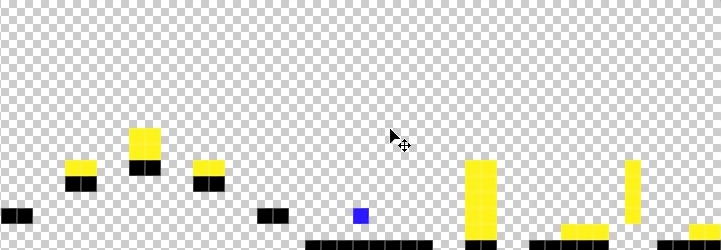
\includegraphics[width=1\textwidth]{pics/leveleditor_designarts_levelcreation.png}}
    \end{minipage}
    \hfill
    \begin{minipage}[t]{0.49\textwidth}
         \subfloat[Das erstellte Level im Spielmodus]{ \label{leveleditor_designarts_gameplay}
        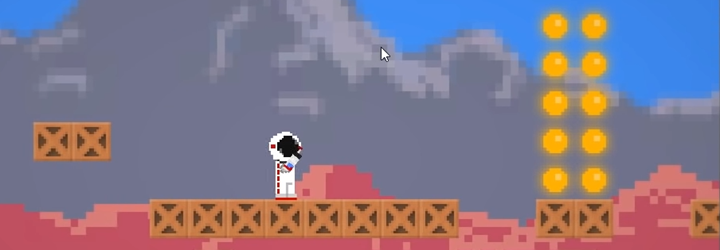
\includegraphics[width=1\textwidth]{pics/leveleditor_designarts_gameplay.png}}
    \end{minipage}
    \caption[Ein in Unity oft implementierter Level-Editor]{Ein in Unity oft implementierter Level-Editor\cite{Brackeys.2017}}
\end{figure} 

In diesem Beispiel wurde für jeden gelben Pixel eine Goldmünze zum einsammeln, für jeden schwarzen Pixel ein Flurstück zum gehen und für einen blauen Pixel die Spielerstartposition gewählt. Diese Möglichkeit des Level-Editors schaut zunächst verblüffend einfach und für jedes 2D-Spiel geeignet aus. Jedoch hat dieser Ansatz einen sehr großen Nachteil:

Für jeden möglichen Zustand eines Objektes muss prinzipiell eine eigene Farbe definiert werden. Dies bedeutet, dass alleine eine beliebig einstellbare Magazingröße einer Waffe theoretisch unendlich viele Farben zur Folge hat. Indem man die Anzahl der möglichen instanziierbaren Zustände eines Objektes beschränkt kann man diesem Problem etwas entgegenwirken. Begrenzt man die Anzahl der einstellbaren Magazingrößen auf drei verschiedene Größen für jede Waffe so erhält man für 10 Waffen 30 unterschiedliche Farben. Berücksichtigt man dabei, dass ein Feind jede beliebige Waffe oder keine tragen kann, so müssen bereits bei 3 Gegnern und dem Spieler (4 * (30 + 1)) = 124 verschiedene Farben definiert werden. Aus diesen Überlegungen ist bereits erkennbar, dass die Anzahl der zu definierenden Farben bei einer Erweiterung des Spiels sehr stark anwächst. Bereits bei über 100 verschiedenen Farben verliert ein Benutzer schnell die Übersicht. Dieses Problem wird noch verstärkt, wenn berücksichtigt werden muss, dass sich Objekte auch überlappen können. Aufgrund dieser extrem schlechten Erweiterbarkeit und Benutzerunfreundlichkeit bei größeren Spielen wurde diese Variante nicht implementiert.

%-- Unity Erweitung für Entwickler-LevelEditor: Erklärung, Begründung, wieso diese Variante nicht hergenommen wurde (alpha-Stand, Editor ist nur für Entwickler gedacht)  Eine andere Möglichkeit eines Leveleditors wird in der neuesten Version von Unity angeboten. Bei dieser Variante kann im Unity-Editor können Objekte zu einem neuen Panel eingestellt werden. Im Anschluss können diese Objekte ausgewählt und in einer Szene platziert werden. 

In Unity gibt im \textit{Asset Store} ebenfalls bereits fertige Level-Editoren zu finden. Der \textit{Asset Store} ist eine von Unity bereitgestellte Plattform, auf dem Entwickler \texttt{Assets} für andere Entwickler zur Verwendung im Spiel anbieten. \textit{Assets} können \textit{Prefabs}, aber auch Sammlungen von unterschiedlichen Arten von \textit{Prefabs} oder sogar in Unity integrierbare Softwarekomponenten wie Level-Editoren sein. Diese Editoren sind jedoch nur sehr schlecht für das bereits existierende Spiel geeignet, da bei diesen oftmals bereits Spielobjekte enthalten sind, die optisch nicht zum Spiel passen und ein großer Umbau dieser Level-Editoren stattfinden muss, um diese für das Spiel nutzen zu können. Hierzu sind Level-Editoren meist nur für Entwickler gedacht, da ein Spieler diese im Spiel nicht nutzen kann.

Dem entgegengesetzt wurde bei dem Design für den Level-Editor ein Editor zur Nutzung für Entwickler als auch Benutzer entwickelt. Ziel ist es, dass nicht nur ein Entwickler, sondern auch jeder Benutzer des Spiels die Möglichkeit haben soll, ein eigenes Level zu erstellen. Dies erlaubt eine viel größere Vielfalt an Leveln, erhöht die Menge des Spielinhalts für einen Benutzer und verringert gleichzeitig den Entwicklungsaufwand zum Erstellen von neuen herausfordernden Leveln. Dabei wurden zunächst folgende Anforderungen für den Level-Editor definiert:

\begin{enumerate}
	\item \textbf{Effizienz:} Dem Benutzer muss es möglich sein schnellstmöglich ein spielbares Level zu erstellen oder zu bearbeiten.
	\item \textbf{Benutzerfreundlichkeit:} Der Benutzer muss  komfortabel und intuitiv ohne Anleitung sofort ein Level erstellen können.
	\item \textbf{Erweiterbarkeit:} Es soll mit geringen Aufwand möglich sein bereits in das Spiel implementierte Elemente wie neue Waffen in den Level-Editor zu integrieren.
	\item \textbf{Geringe Abhängigkeiten}: Der Level-Editor stellt einen eigenen Bereich des Spiels dar. Änderungen an dem Level-Editor (und umgekehrt), mit Ausnahme der Änderung an Schnittstellen zu gemeinsamen Komponenten, sollen den jeweils anderen Bereich der Software nicht beeinträchtigen.
\end{enumerate}

Diese Anforderungen stellen sicher, dass der Benutzer gut mit dem Level-Editor arbeiten kann und somit die Bereitschaft erhöhen neue Level zu erstellen und diese mit der Gemeinschaft der Spieler und Entwickler zu teilen. Anforderung 3 stellt sicher, dass ein Entwickler kaum Aufwand betreiben muss, um ein neues Element für den Level-Editor benutzbar zu machen. Mit der letzten Anforderung soll bewirkt werden, dass Änderungen an einer Komponente die Funktionalität der jeweils anderen nicht beeinträchtigen.

\subsection{Die Benutzeroberfläche}\label{sec:user_interface}
Für die Implementierung musste ein Weg gefunden werden, um all diese Anforderungen umzusetzen. Dabei wurden zunächst Eigenschaften des Level-Editors definiert, die dem Benutzer es ermöglichen sollen besonders effizient und intuitiv ein Level zu erstellen oder zu bearbeiten. Folgende Eigenschaften wurden zur Kontrolle der Einhaltung der Anforderungen definiert:

\begin{itemize}
	\item Der Benutzer soll eine Rückmeldung erhalten, welches Objekt er bei Mausklick editieren kann.
	\item Der Benutzer soll ein Objekt per Mausklick verschieben können. Dabei soll ihm vorher angezeigt werden, welches Objekt er aktuell verschieben würde.
	\item Der Benutzer soll mit Hilfe des Verschiebens einer Waffe einen Gegner oder Spieler mit dieser bewaffnen können.
	\item Der Benutzer soll per Klick auf eine Schaltfläche, das auf der Schaltfläche angegebene Spielobjekt bei der Maus angezeigt bekommen und bei jedem Mausklick auf der Karte bei der gewählten Position eine Instanz des dort angezeigten Spielobjektes erstellen können.
	\item Mit einem Mausklick auf ein bereits platziertes Objekt sollen änderbare Eigenschaften wie Munitionsmenge bei Waffen angezeigt und durch den Benutzer leicht verändert werden können.
	\item Für Levelelemente wie Wände soll es möglich sein bei gedrückter Maustaste und gleichzeitigem Bewegen der Maus bei den Positionen des Mauszeigers automatisch Spielobjekte des ausgewählten Typs zu platzieren.
	\item Ein auf die Karte gesetztes Objekt soll ohne Änderung direkt bei Speicherung des Levels im zugehörigen Spiel verwendet werden können.
	\item Es soll möglich sein komfortabel mit der Kamera hinein- und herauszuzoomen, als auch die Position der Kamera zu ändern.
\end{itemize}

Die Interaktion des Benutzers mit dem Level-Editor geschieht durch die Benutzeroberfläche des Editors, die im Folgenden vorgestellt wird. Mit ihr und der damit verbundenen Anwendungslogik werden diese Eigenschaften erfüllt. 

\subsubsection{Die Benutzeroberfläche}
\begin {figure}[h]
	\begin {center}
	    \includegraphics[width=1\textwidth]{pics/leveleditor_interface.png}
		\caption{Die Benutzeroberfläche des Level-Editors}
		\label{fig:userinterface_leveleditor}
	\end {center}
\end {figure}

Abbildung \ref{fig:userinterface_leveleditor} zeigt die Benutzeroberfläche des Level-Editors. Diese ist unterteilt in den Le\-vel\-ver\-wal\-tungs-Bereich (links oben), den Objekterstellungs- und Lösch-Bereich (links am Rand) und den Objektbearbeitungs-Bereich (rechter Rand). 

Mit dem Levelverwaltungsbereich kann ein neues Level erstellt, ein Level geladen oder gespeichert werden. Zum Erstellen eines neuen Levels können die Textfelder \glqq{}W\grqq{} für Weite und \glqq{}H\grqq{} für Höhe genutzt werden, um die Größe des neuen Levels festzulegen und mit der Schaltfläche \glqq{}New Level\grqq{} wird dieses erstellt. Das aktuell im Editor vorhandene Level mit allen Spielobjekten wird dabei ohne Sicherung gelöscht und durch das neue Level ersetzt. Sollen die Änderungen behalten werden, so ist es wichtig das Level vorher zu speichern, um dieses mit Hilfe der gespeicherten Datei wieder in den Editor laden zu können.

Mit dem Objekterstellungs- und Lösch-Bereich können neue Spielobjekte erstellt oder bereits im Level vorhandene Objekte gelöscht werden. Hierfür muss die Schaltfläche für das zugehörige Objekt gedrückt und das ausgewählte Objekt mit der Maus auf die gewünschte Position auf der Karte mit einem Mausklick gesetzt werden. Möchte man ein Objekt löschen, so muss analog die Schaltfläche \glqq{}Deletion Mode\grqq{} gedrückt und auf das zu löschende Objekt auf der Karte mit der linken Maustaste geklickt werden.

Im Objektbearbeitungs-Bereich können Eigenschaften von Objekten bearbeitet werden. Letzterer wird sichtbar, wenn im Level-Editor auf ein markiertes Objekt geklickt wird und der Lösch- oder Platzierungsmodus nicht aktiviert ist. Hier werden für jedes Objekt spezifische Eigenschaften zum Einstellen angezeigt. Beispielsweise ist es möglich für einen Gegner eine Patroullienroute zu erstellen oder die Munitionsmenge für eine bestimmte Waffe festzulegen. Im Bild \ref{fig:userinterface_leveleditor} ist letzteres sichtbar. 

Es ist zu erwähnen, dass jedes Level bei Erstellung eine Wandumrandung an den Kanten des Levels erhält, die nicht gelöscht oder verschoben werden können. Dies wurde festgelegt, da ein Spieler oder andere Spielobjekte sich nicht über den Rand der Karte hinaus bewegen sollen.

Die Interaktion des Benutzers mit dem Level-Editor funktioniert mit Hilfe der beiden Maustasten, dem Bewegen der Maus und dem Mausrad. mit dem Mausrad kann aus der Karte hinein- und herausgezoomt werden. Wird die rechte Maustaste nur kurz gedrückt, so wechselt der Editor in den sogenannten \glqq{}Leermodus\grqq{}. Dies bedeutet der Editor verlässt den aktuellen Zustand und wechselt in den Startzustand, bei dem Objekte nicht verändert, platziert oder gelöscht werden können. Wird die rechte Maustaste gedrückt gehalten und die Maus bewegt, so kann zu einem anderen Ort der Karte mit der Kamera navigiert werden. Die linke Maustaste hat je nach Zustand eine andere Bedeutung:

\begin{itemize}
	\item \textbf{Leermodus:} 	
	\begin {itemize}
	\item Tastendruck ein markiertes Objekt: Wechsel in den Editiermodus
	\item Tastendruck auf eine freie Fläche der Karte: Keine Wirkung
	\item Auf ein markiertes Objekt wird geklickt, gehalten und die Maus bewegt: Die Position des Spielobjektes auf der Karte wird verändert
	\end{itemize}
	\item \textbf{Platzierungsmodus:} 
	\begin{itemize}
	\item Tastendruck auf ein Stück der Karte ohne Level-Element: ein neues Spielobjekt wird an der Position des Mauszeigers platziert.
	Tastendruck auf ein Stück der Karte mit Level-Element: Keine Wirkung
	\item Gedrückt halten: Ist das ausgewählte Spielobjekt ein Level-Element, so werden, wenn möglich, an den Positionen des Mauszeigers Instanzen des ausgewählten Spielobjektes erstellt.
	\end{itemize} 
	\item \textbf{Editiermodus:} 
	\begin{itemize}
	\item Tastendruck auf ein Spielobjekt: Aktualisierung des Objektbearbeitungsbereiches für das ausgewählte Spielobjekt
	\item Tastendruck auf einen leeren Fleck der Karte: Wechsel in den Leermodus und Verbergen des Objektbearbeitungsbereiches
	\end{itemize} 
	\item \textbf{Löschmodus}: 
	\begin{itemize}
	\item Tastendruck auf ein markiertes Objekt: Löschen des Objektes
	\item Gedrückt halten: Jedes Spielobjekt das markiert wird, wird sofort gelöscht.
	\end{itemize}
	\item \textbf{Modus zum Setzen von Patroullienrouten}: 
	\begin{itemize}
	\item Tastendruck Auf ein Stück der Karte ohne Level-Element: Setzen eines Wegpunktes
	\item Tastendruck Auf ein Stück der Karte mit Level-Element: Keine Wirkung
	\end{itemize}  
\end{itemize}

Wird im Modus für das Setzen der Patroullienroute eines Gegners dieser Modus verlassen, so wird die für den Gegner bis dahin gesetzte Patroullienroute gespeichert. Das Arbeiten mit diesen Zuständen soll die Steuerung des Level-Editors für den Benutzer erleichtern, da ansonsten unnötig viele Tasten für unterschiedliche Funktionalität belegt werden müssten. Für Details zur Umsetzung des Level-Editors wird auf die im nachfolgenden Abschnitt vorgestellte Implementierung verwiesen.

%Mit Hilfe des Levelverwaltungs-Bereiches kann ein neues Level mit einer beliebigen Größe erstellt, ein bereits existierendes Level zum Editieren geladen oder ein bereits erstelltes Level gespeichert werden.

%Beim Drücken der Schaltfläche "Neues Level" werden die in den Textfeldern vorhandenen Werte ausgelesen und die Funktion CreateLevel(...) des LevelCreators übergeben. 


%Bei Klick auf einer dieser Schaltflächen wird das Flag für den Platzierungsmodus gesetzt und eine Instanz des ausgewählten Prefabs erstellt welches der Maus folgt. Bei einem Mausklick auf die Karte wird dort wo sich das der Maus folgende SpielObjekt befindet ein weiteres Objekt dieser Art instanziiert, in das Verzeichnis für die auf der Karte befindlichen Spielobjekte eingetragen (inScenePlacedObjects). Da sich Levelelemente und Objekte anderen Typs nicht gleichzeitig auf einem Kartenstück befinden können, wird hinterlegt auf welchem Kartenstück sich das Spielobjekt befindet.


%Wird die Schaltfläche für das Laden eines Levels gedrückt, so ruft der InterfaceButtonHandler die Funktion LoadLevel() des LevelCreators auf, welcher den Befehl zum Laden der Daten an den LevelController mit Hilfe der Funktion LoadLevelData() übergibt und danach die Daten mit Hilfe des LevelDatenManagers mit Hilfe der Funktion GetLevelData() abruft und dem Modul LevelPlacement über die Funktion PlaceObjects(...) die SpielObjekte für das Level erstellen und platzieren lässt.    

%Wird die Schaltfläche zum Speichern des Levels gedrückt, so ruft der InterfaceButtonHandler die Funktion SaveLevel() des LevelCreators auf, welche die auf der Karte platzierten Objekte dem LevelDataManager mit Hilfe der Funktion SaveLevelData(...) zum Speichern übergibt und nach der Speicherung der Objekte dem LevelController den Befehl zur Serialisierung der Spielobjekte mit Hilfe der Funktion SaveLevel() übergibt. 

%Wird auf ein Objekt mit der Maus geklickt ohne im Lösch- oder Platzierungsmodus zu sein wird das Flag für den Editiermodus gesetzt. Wird auf ein anderes Objekt geklickt so wird das neu ausgewählte Objekt bearbeitet. Wird hingegen auf kein Objekt geklickt, so wird der Editiermodus verlassen und es wird weder ein Objekt erstellt, gelöscht oder bearbeitet. Wird ein Gegner ausgewählt so können die Wegpunkte für diesen Gegner gesetzt werden. Hierfür muss im zu dem zugehörigen Objekteditorfenster in der Benutzeroberfläche die Schaltfläche "Start" zum Starten des WegPlatzierungsmodus gedrückt werden. Wird dieser gedrückt, so können über einen Klick auf die Karte die Wegpunkte nacheinander für den Gegner gesetzt werden. Wird auf die Schaltfläche "Stop" gedrückt oder einer der anderen Modusse über das Drücken der jeweiligen Schaltfläche gestartet, so wird werden die aktuell gesetzten Wegpunkte in dem Gegner-Spielobjekt gespeichert. 

%Im Objektbearbeitungsbereich können Levelelemente, Gegner und Waffen erzeugt, gelöscht oder bearbeitet werden. Im InterfaceManager sind diese in die zwei Benutzerbereiche Objektbearbeitung und Objekterstellung/-löschung unterteilt. Abbildung \ref{fig:object_management} zeigt den dazugehörigen internen Aufbau. Aus Gründen der Übersichtlichkeit wurden im LevelCreator Abhängigkeiten zu anderen Komponenten und Attribute in der Klasse PlacedObject weggelassen, die aus dem zugehörigen Interface ersichtlich sind. 

\subsection{Die Implementierung}\label{sec:implementation}
\begin {figure}[h]
	\begin {center}
	    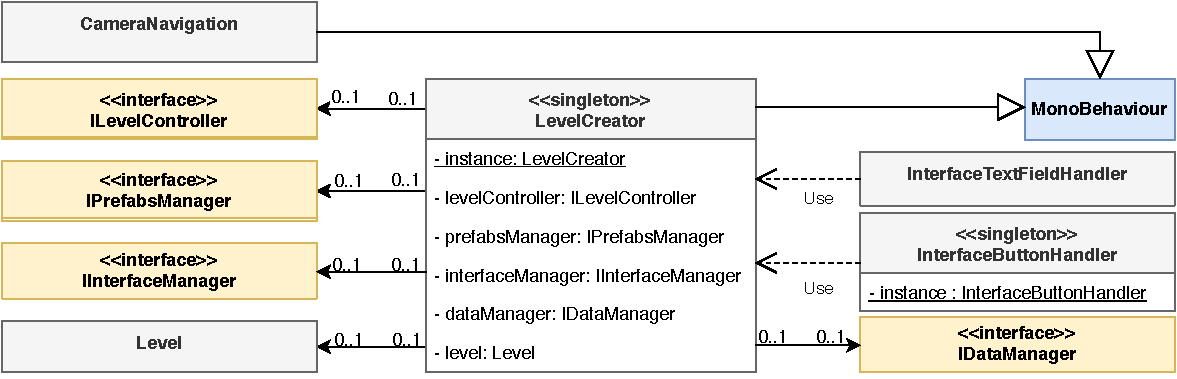
\includegraphics[width=1\textwidth]{pics/leveleditor_core.pdf}
		\caption{Der Level-Editor mit seinen Kernkomponenten}
		\label{fig:leveleditor_core}
	\end {center}
\end {figure}

Der Level-Editor stellt einen eigenständigen Bereich des Spiels dar. Für die Umsetzung des Editors konnten folgende Aufgabenbereiche identifiziert werden:

\begin{itemize}
	\item Die Ereignisbehandlung: Die Kommunikation der Komponenten bei Benutzeraktionen
	\item Die Kameranavigation
	\item Die Verwaltung der \textit{Prefabs}	
	\item Die Verwaltung und Aktualisierung der Benutzeroberfläche
	\item Die Datenverwaltung
	\item Das Platzieren, Löschen und Editieren von Spielobjekten
	\item Das Laden und Speichern eines Levels
\end{itemize} 

Für jeden dieser Aufgabenbereiche wurde eine eigenständige Komponente entwickelt. Abbildung \ref{fig:leveleditor_core} zeigt die Abhängigkeiten der Kernkomponente \texttt{LevelCreator} zu den anderen intern verwendeten Komponenten. Dieses \textit{UML}-Diagramm soll einen Überblick über die Kernkomponenten des Level-Editors geben. Hierfür wurden die Methoden der zu den Komponenten gehörigen Interfaces und Klassen weggelassen. Der \texttt{LevelCreator} stellt die zentrale Komponente dar, die zusätzlich zu seiner eigenen Funktionalität sich auch um die Weiterleitung von Informationen an die anderen Komponenten kümmert. Um ein sogenanntes Gottobjekt, ein Objekt das alles weiß, zu vermeiden wurde für jeden Aufgabenbereich eine eigenständige Komponente entwickelt und jeder dieser Komponenten wird ausschließlich über die in der Abbildung dargestellten Schnittstellen nach dem \textit{Facade}-Entwurfsmuster\cite{Gamma.2011} angesprochen. Tabelle \ref{table:task_component_association} zeigt die Zuordnung der Aufgabengebiete zu den Komponenten.

\begin{table}[h]
\begin {tabularx}{\linewidth}{
    | >{\hsize=1.0\hsize}X| % 50% of 2\hsize 
    >{\hsize=1.0\hsize}X|% 50% of 2\hsize 
       % sum=2.0\hsize for 2 columns
  }
  \hline
  	    \textbf{Aufgabengebiet} & \textbf{Komponente} \\ [1.0ex]
		\hline
		 Die Ereignisbehandlung & \texttt{InterfaceButtonHandler/ TextFieldHandler} \\[0.5ex]
		 \hline
		 Die Kameranavigation & \texttt{CameraNavigation} \\[0.5ex]
		 \hline
		Die Verwaltung der \textit{Prefabs} & \texttt{PerfabsManager} \\[0.5ex] \hline
		 Die Verwaltung und Aktualisierung der Benutzeroberfläche & \texttt{InterfaceManager} \\[0.5ex]
		 \hline
		 Die Datenverwaltung & \texttt{DataManager} \\[0.5ex]
		 \hline
		Das Platzieren, Löschen und Editieren von Spielobjekten & \texttt{LevelCreator} \\[0.5ex]
		\hline
		Laden und Speichern eines Levels & \texttt{LevelController} \\[0.5ex]
		\hline
\end{tabularx}
\caption{Die Zuordnung der Aufgabengebiete zu den verwendeten Komponenten}
\label{table:task_component_association}
\end{table}

Durch das Einführen von Interfaces zwischen diesen Komponenten, werden die Abhängigkeiten der Komponenten voneinander auf ein Minimum reduziert. Zusätzlich wurde eine Hierarchie eingeführt, um zyklische Abhängigkeiten zu verhindern. Die einzigen Komponenten die auf den \texttt{LevelCreator} zugreifen sind die Komponenten für die Ereignisbehandlung und auch nur dann, wenn der Benutzer ein Ereignis beispielsweise durch das Drücken einer Schaltfläche ausgelöst hat. Der \texttt{LevelCreator} leitet die für die anderen Kernkomponenten benötigten Informationen weiter und kümmert sich um die Koordination und Initialisierung dieser Komponenten.

Im Folgenden wird die Implementierung für die verschiedenen Komponenten vorgestellt. Dabei werden diese nach der folgenden Reihenfolge vorgestellt:

\begin{enumerate}
	\item Die Ereignisbehandlung
	\item Die Kameranavigation
	\item Der Begriff \textit{Prefab} im Level-Editor
	\item Die Verwaltung der \textit{Prefabs}	
	\item Die Verwaltung und Aktualisierung der Benutzeroberfläche
	\item Das Platzieren, Löschen und Editieren von Spielobjekten
	\item Die Datenverwaltung und das Laden und Speichern eines Levels
\end{enumerate} 

\subsubsection{Die Ereignisbehandlung: Die Kommunikation der Komponenten bei Benutzeraktionen} \label{chapter:eventmanagement}
\begin {figure}[h]
	\begin {center}
	    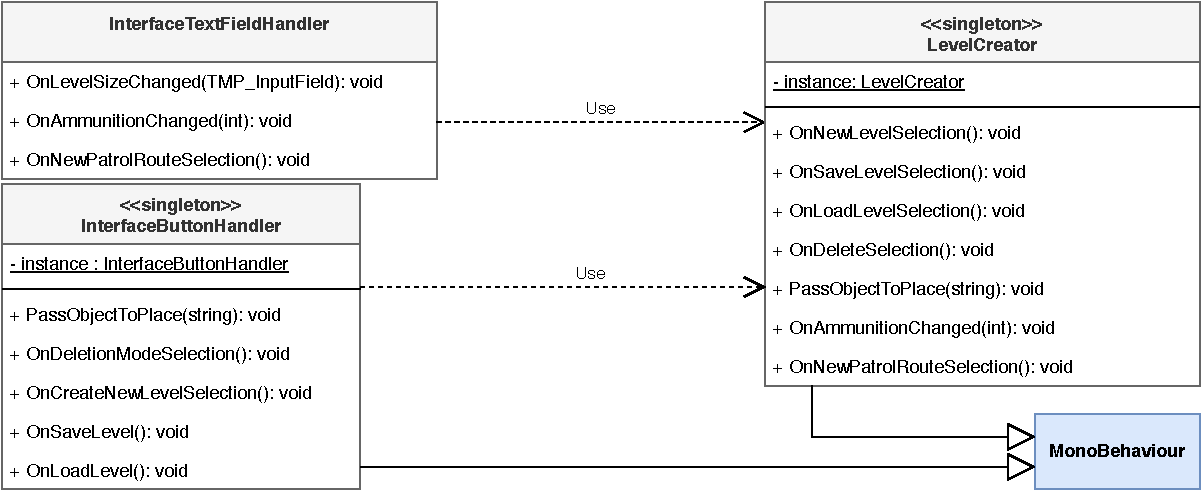
\includegraphics[width=1\textwidth]{pics/leveleditor_eventhandler.pdf}
		\caption{Die Ereignisbehandlung des Level-Editors}
		\label{fig:eventhandler}
	\end {center}
\end {figure}

Abbildung \ref{fig:eventhandler} zeigt die beteiligten Komponenten für die Ereignisbearbeitung. Es gibt zwei Komponenten, die Ereignisse abfangen: Der \texttt{InterfaceTextFieldHandler} für Ereignisse ausgelöst von Textfeldern und der \texttt{InterfaceButtonHandler} für Ereignisse ausgelöst durch das Drücken von Schaltflächen. Dabei gibt es folgende Fälle bei denen Ereignisse ausgelöst werden:

\begin{enumerate}
	\item Änderung des Textfeldes für die Weite oder Höhe eines neuen Levels
	\item \glqq{}New Level\grqq{}-Schaltfläche drücken
	\item \glqq{}Deletion Mode\grqq{}-Schaltfläche wird gedrückt
	\item Drücken einer Schaltfläche zum Platzieren eines Spielobjektes auf die Karte
	\item Änderung der Munitionsmenge im Objekt-Editor Bereich
	\item Erstellung oder Löschung einer Patroullienroute eines Spielobjektes
	\item \glqq{}Load Level\grqq{}-Schaltfläche drücken
	\item \glqq{}Save Level\grqq{}-Schaltfläche drücken
\end{enumerate}

In allen Fällen wird immer eine Funktion des \texttt{LevelCreators} aufgerufen, welcher die Bearbeitung dieser Aufgabe an andere Module übergibt und im Fall mehrerer beteiligten Komponenten sich um die schrittweisige Bearbeitung dieser Aufgabe kümmert.

Von dieser Regel gibt es nur eine einzige Ausnahme: Der erste Fall. Bei der Änderung des Textes in den Textfeldern für die Weite oder Höhe eines neuen Levels wird der \texttt{LevelCreator} und auch sonst keine andere Komponente miteinbezogen. Ein von Unity integrierter Validator kümmert sich darum, dass nur \textit{integer} Werte im zweistelligen Wertebereich eingegeben werden dürfen, während der \texttt{InterfaceTextfieldhandler} selbst überprüft, ob der neu eingegebene Wert im Wertebereich von 10 bis 99 liegt. Falls dem nicht so ist, so wird der Wert auf den Standardwert 30 gesetzt.

Beim Drücken der Schaltfläche \glqq{}New Level\grqq{} werden die in den Textfeldern vorhandenen Werte ausgelesen und der Funktion \texttt{OnNewLevelSelection(...)} des \texttt{LevelCreators} übergeben. Dieser löscht daraufhin das vorhandene Level und erstellt mit den übergebenen Werten ein Neues.

In den Fällen 3 und 4 wechselt der \texttt{Level-Editor} in den Zustand Löschmodus für das Löschen von Spielobjekten oder in den Platziermodus und zeigt das auf der Karte platzierbare Spielobjekt bei dem Mauszeiger an.

Das Erstellen oder Löschen der Patroullienroute oder die Änderung der Munitionsmenge findet im Objekteditier-Bereich der Benutzeroberfläche statt.  
Die Änderung der Munitionsmenge führt zum Aufruf der Funktion \texttt{OnAmmunitionChanged()} des \texttt{LevelCreators}, welcher die Munitionsmenge mit Hilfe eines eigenen Moduls \texttt{Objekteditier-Modul} des Objektes anpasst und dem \texttt{InterfaceManager} das aktualisierte Objekt zur Aktualisierung der Benutzeroberfläche übergibt.

Beim Aufruf der Funktion \texttt{OnNewPatrolRouteSelection()} hingegen, ausgelöst durch die Schaltfläche \glqq{}New Patrol Route\grqq{}, gibt der \texttt{LevelCreator} seinem Modul \texttt{ObjectDeletionModule} die Anweisung zum Löschen der Patroullienroute und versetzt ihn in den Modus für das Setzen einer neuen Patroullienroute. 

Die Bearbeitung der letzten beiden Fälle wird im Abschnitt \glqq{}Die Datenverwaltung und das Laden und Speichern eines Levels\grqq{} erklärt.

\subsubsection{Die Kameranavigation}
\begin {figure}[h]
	\begin {center}
	    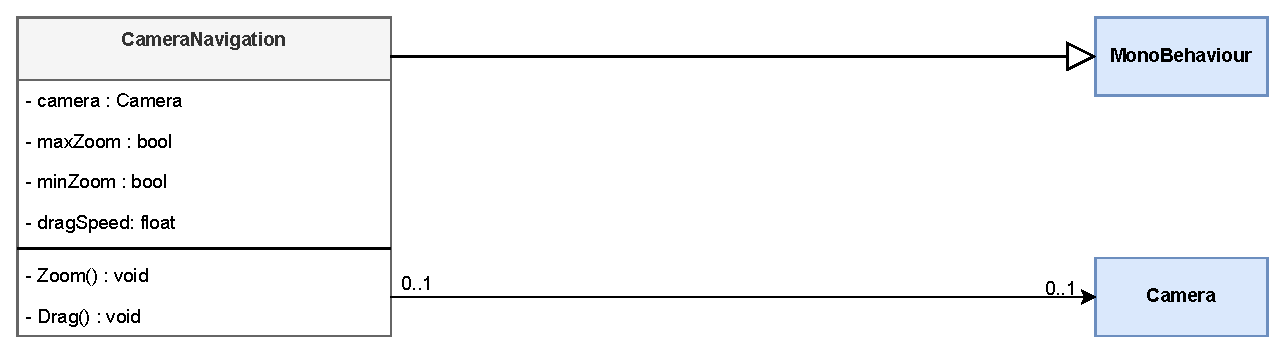
\includegraphics[width=1\textwidth]{pics/leveleditor_cameranavigation.eps}
		\caption{Die Kameranavigation im Level-Editor}
		\label{fig:leveleditor_cameranavigation}
	\end {center}
\end {figure}
Die Kameranavigation kontrolliert die Kamera des Level-Editors. Wie bereits beschrieben ist es im Level-Editor möglich über das Scrollen mit dem Mausrad zu einem Punkt der Karte hinein- und wieder herauszuzoomen. Hierfür wird intern die Funktion \texttt{Zoom()} verwendet. Desweiteren kann bei gedrückt halten der rechten Maustaste und Änderung gleichzeitigem Bewegen der Maus die Position der Kamera geändert und so ein anderer Ort der Karte bearbeitet werden. Hierfür wird die Funktion \texttt{Drag()} genutzt.


\subsubsection{Der Begriff \textit{Prefab} im Level-Editor}
\begin {figure}[h]
	\begin {center}
	    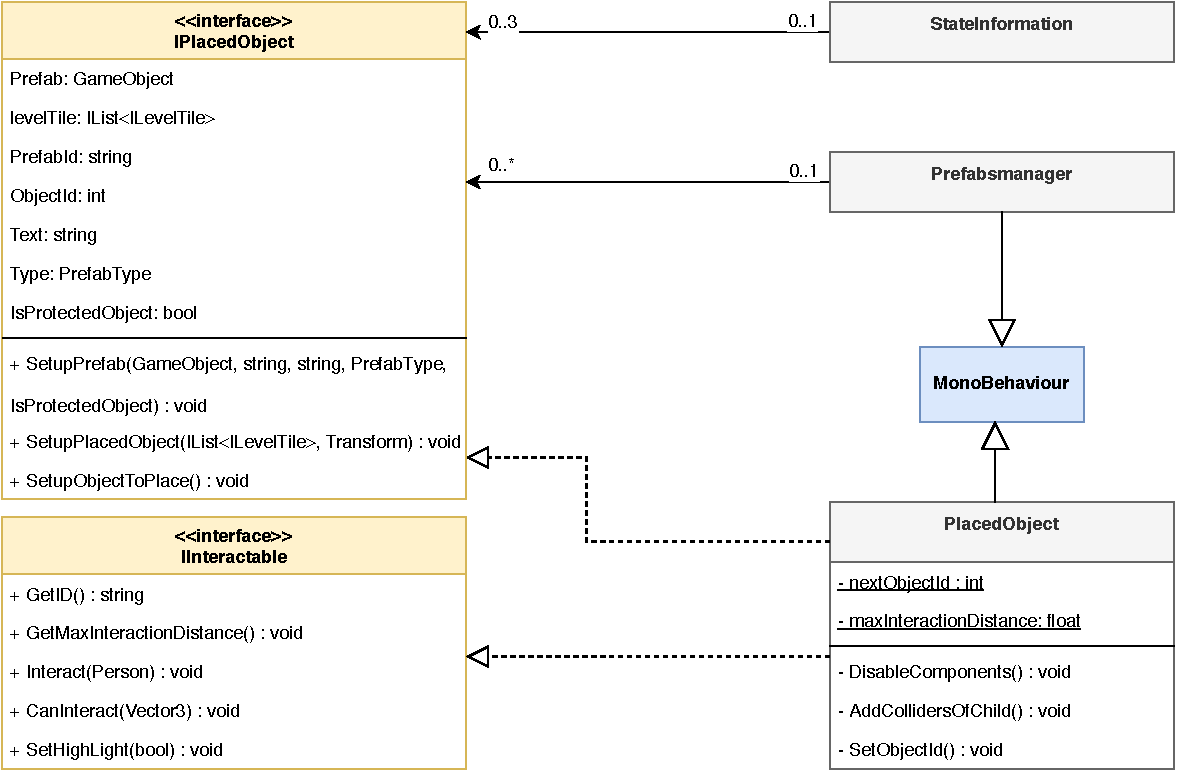
\includegraphics[width=1\textwidth]{pics/leveleditor_placedobject.pdf}
		\caption{Der Aufbau des verwendeten Containerobjekt \texttt{PlacedObject}}
		\label{fig:leveleditor_placedobject}
	\end {center}
\end {figure}

Um auf ein bestimmtes Objekt einzuwirken, ob es zu löschen, bearbeiten oder zu verschieben, ist es zunächst nötig dafür zu sorgen, dass der Benutzer weiß welches Objekt die Aktion betrifft. Hierfür kann der bereits implementierte \texttt{InteractableHoverHandler} benutzt werden. Durch diesen wird ein Objekt blau hinterlegt, wenn er mit der Maus über dieses Objekt fährt und mit Hilfe des \texttt{InteractableProximityChecker} kann auf dieses Objekt zugegriffen werden. Um diese Komponenten im Level-Editor nutzen zu können, muss jedes Objekt, das markiert werden soll das Interface \texttt{IInteractable} implementieren. Im eigentlichen Spiel soll es allerdings nicht vorkommen, dass eine Tür beispielsweise blau markiert wird oder gar verschoben werden kann. Um es trotzdem zu ermöglichen Level-Elemente wie Wände oder Türen und Gegner oder den Spieler markieren zu können, und die Abhängigkeiten des Level-Editors zum eigentlichen Spiel so gering wie möglich zu halten, wurde eine Art Container-Objekt eingeführt. Jedem Spielobjekt egal welchen Typs wurde ein Objekt übergeordnet und bestimmte Komponenten des Spielobjektes deaktiviert, da sonst beim Setzen eines Gegners und eines Spielers der Gegner den Spieler anfangen würde anzugreifen. Dadurch ist es möglich weiterhin auf die spezifischen Eigenschaften der Spielobjekte zuzugreifen, während die Interaktion auf diese Objekte über das Container-Objekt gehandhabt wird. Somit können direkte Abhängigkeiten vermieden werden, was dazu führt, dass für das Platzieren und Verwalten von Spielobjekten im Level egal ist, um welches Spielobjekt es sich genau handelt. 

Abbildung \ref{fig:leveleditor_placedobject} zeigt den internen Aufbau dieses Container-Objektes. Durch die Implementierung des Interfaces \texttt{IInteractable} und die Verlagerung des \textit{Colliders} des Spielobjektes zum Container-Objekt werden nicht mehr die durch das Interface importierten Funktionen des Spielobjektes aufgerufen, sondern die des Container-Objektes. Dadurch ist es auch mit der Methode \texttt{Interact()} möglich einem Gegner oder Spieler eine Waffe zu geben oder die Spielobjekte auf der Karte zu verschieben. Da ein \textit{Collider} nur ein Spielobjekt besitzen kann, muss das Container-Objekt von der Unity-Klasse \textit{MonoBehaviour} erben. Aus Gründen der Übersichtlichkeit wurden die aus den Interfaces importieren ersichtlichen Attribute und Methoden im Container-Objekt weggelassen. 

Das Container-Objekt hat folgende Attribute:

\begin{itemize}
	\item \textbf{objectId:} Die Objekt-Id mit der jedes platzierte Objekt eindeutig identifiziert werden kann.
	\item \textbf{Text:} Der Text der bei der zugehörigen Schaltfläche in der Benutzeroberfläche angezeigt wird.
	\item \textbf{Prefab:} Das untergeordnete Spielobjekt.
	\item \textbf{Type:} Der Typ des Spielobjektes, also ob es sich um ein Level-Element, Spieler, Gegner oder eine Waffe handelt.
	\item \textbf{LevelTile:} Auf welchem Stück oder Stücken der Karte das Spielobjekt platziert ist 
	\item \textbf{PrefabId:} Der Identifikator mit dem bei Klick auf eine Schaltfläche für das Setzen eines \textit{Prefabs} festgestellt werden kann, welches \textit{Prefab} ausgewählt wurde. Diese ID wird dem \texttt{PrefabsManager} übergeben, um eine Instanz des zugehörigen \textit{Prefabs} zu erhalten.
	\item \textbf{IsProtedObject:} Dieses Flag legt fest, ob das Objekt gelöscht oder verändert werden darf. Dies ist für die Randbegrenzung wichtig, da dort Wände nicht verschoben oder sogar gelöscht werden dürfen.
\end{itemize}

Der Typ des Spielobjektes ist unter anderem wichtig, um später entscheiden zu können, welche Eigenschaften bei dem jeweiligen Spielobjekt zum Ändern angezeigt werden. 

Dieses neue \textit{Prefab} stellt das Objekt dar, mit dem alle Komponenten des Level-Editors arbeiten. Dabei greifen alle Komponenten ausschließlich über das zugehörige Interface \texttt{IPlacedObject} auf dieses \textit{Prefab} zu. Die Komponenten, die eine Referenz auf ein solches Container-Objekt speichern sind der \texttt{LevelCreator} und der \texttt{PrefabsManager}. Der \texttt{LevelCreator} speichert in seinem Objekt \texttt{StateInformation} temporär Instanzen von \textit{Prefabs} ein, um weitere Klone von diesen Erstellen zu können oder diese zu bearbeiten. Der \texttt{PrefabsManager} hingegen verwaltet die eigentlichen \textit{Prefabs}. Dieser wird im nächsten Abschnitt genauer erläutert.

\subsubsection{Die Verwaltung der \textit{Prefabs}}
\begin {figure}[h]
	\begin {center}
	    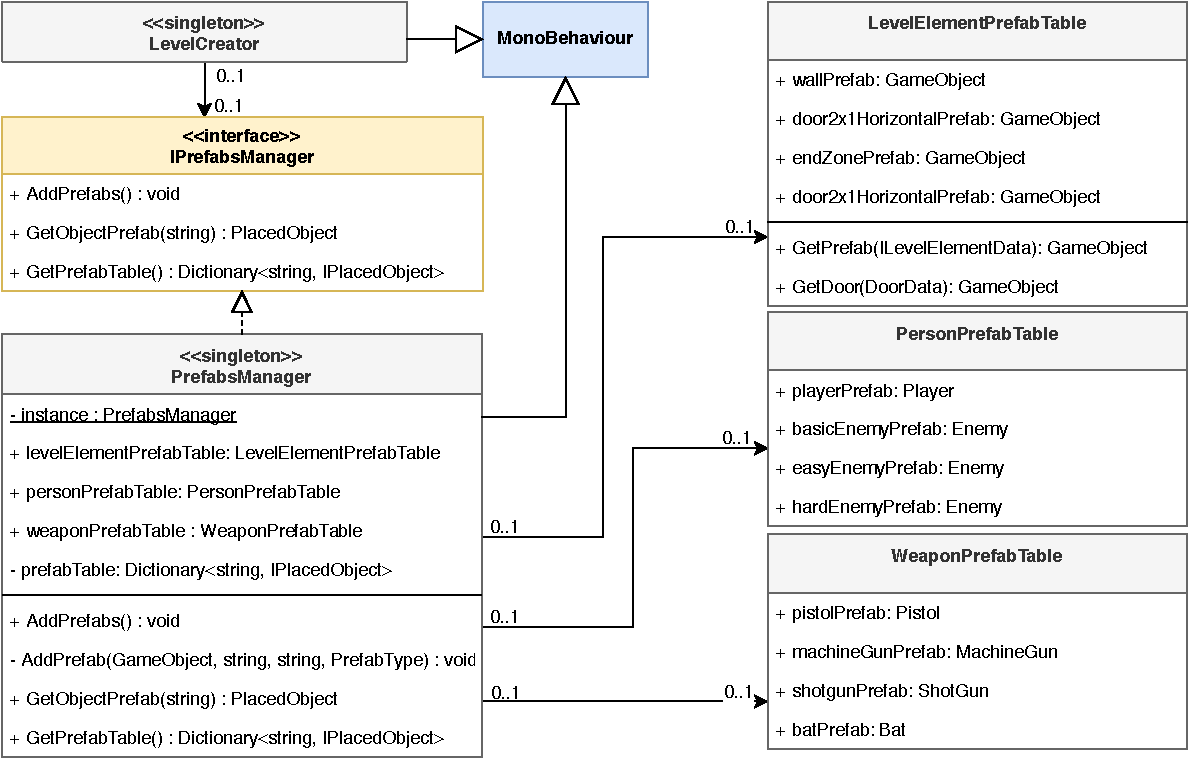
\includegraphics[width=1\textwidth]{pics/leveleditor_prefabsmanager.pdf}
		\caption{Der \texttt{PrefabsManager} des Level-Editors}
		\label{fig:prefabsmanager}
	\end {center}
\end {figure}

Wird der Level-Editor gestartet, so werden als erstes die \textit{Prefabs} für das Erstellen von neuen Spielobjekten geladen und jedes dieser \textit{Prefabs} ein Container-Objekt übergeordnet, das mit Informationen zu diesem \textit{Prefab} angereichert wird. Daraus entsteht ein neues temporär existierendes \textit{Prefab} zur Verwendung im Level-Editor. Das Klassendiagramm in Abbildung \ref{fig:prefabsmanager} gibt einen Überblick über die interne Implementierung des \texttt{PrefabsManager}. Wie zu sehen ist greift der \texttt{PrefabsManager} dabei auf die in den Tabellen \texttt{LevelElementPrefabTable}, \texttt{PersonPrefabTable} und \texttt{WeaponPrefabTable} gespeicherten \textit{Prefabs} zu. Die Funktion \texttt{Add- \linebreak Prefabs()} dient zur Initialisierung der \texttt{PrefabTabelle}. Dadurch kann der \texttt{LevelCreator} die Initialisierung der Komponenten steuern. Die Funktion \texttt{GetPrefabTable()} bewirkt schließlich, dass der \texttt{PrefabsManager} eine Kopie der intern verwendeten Tabelle zur Speicherung und Zuordnung der \textit{Prefabs} übergibt. Diese Kopie wird dem \texttt{IntefaceManager} zur Initialisierung übergeben. 

Neben dem Laden der \textit{Prefabs} kümmert der \texttt{PrefabsManager} sich auch um die Verwaltung dieser. Dabei ist es wichtig, dass die \textit{Prefabs} von Komponenten anderer Aufgabenbereiche zur Laufzeit nicht verändert werden können, da eine Änderung dieser zur Laufzeit auch eine permanente Änderung der in Unity hinterlegten \textit{Prefabs} zur Folge hätte. Daher erstellt der \texttt{PrefabsManager} auf Anfrage eines \textit{Prefabs} mit der Funktion \texttt{GetObjectPrefab(...)} eine neue Instanz des angefragten \textit{Prefabs} und übergibt diese. 

\subsubsection{Die Verwaltung und Aktualisierung der Benutzeroberfläche}

\begin {figure}[H]
	\begin {center}
	    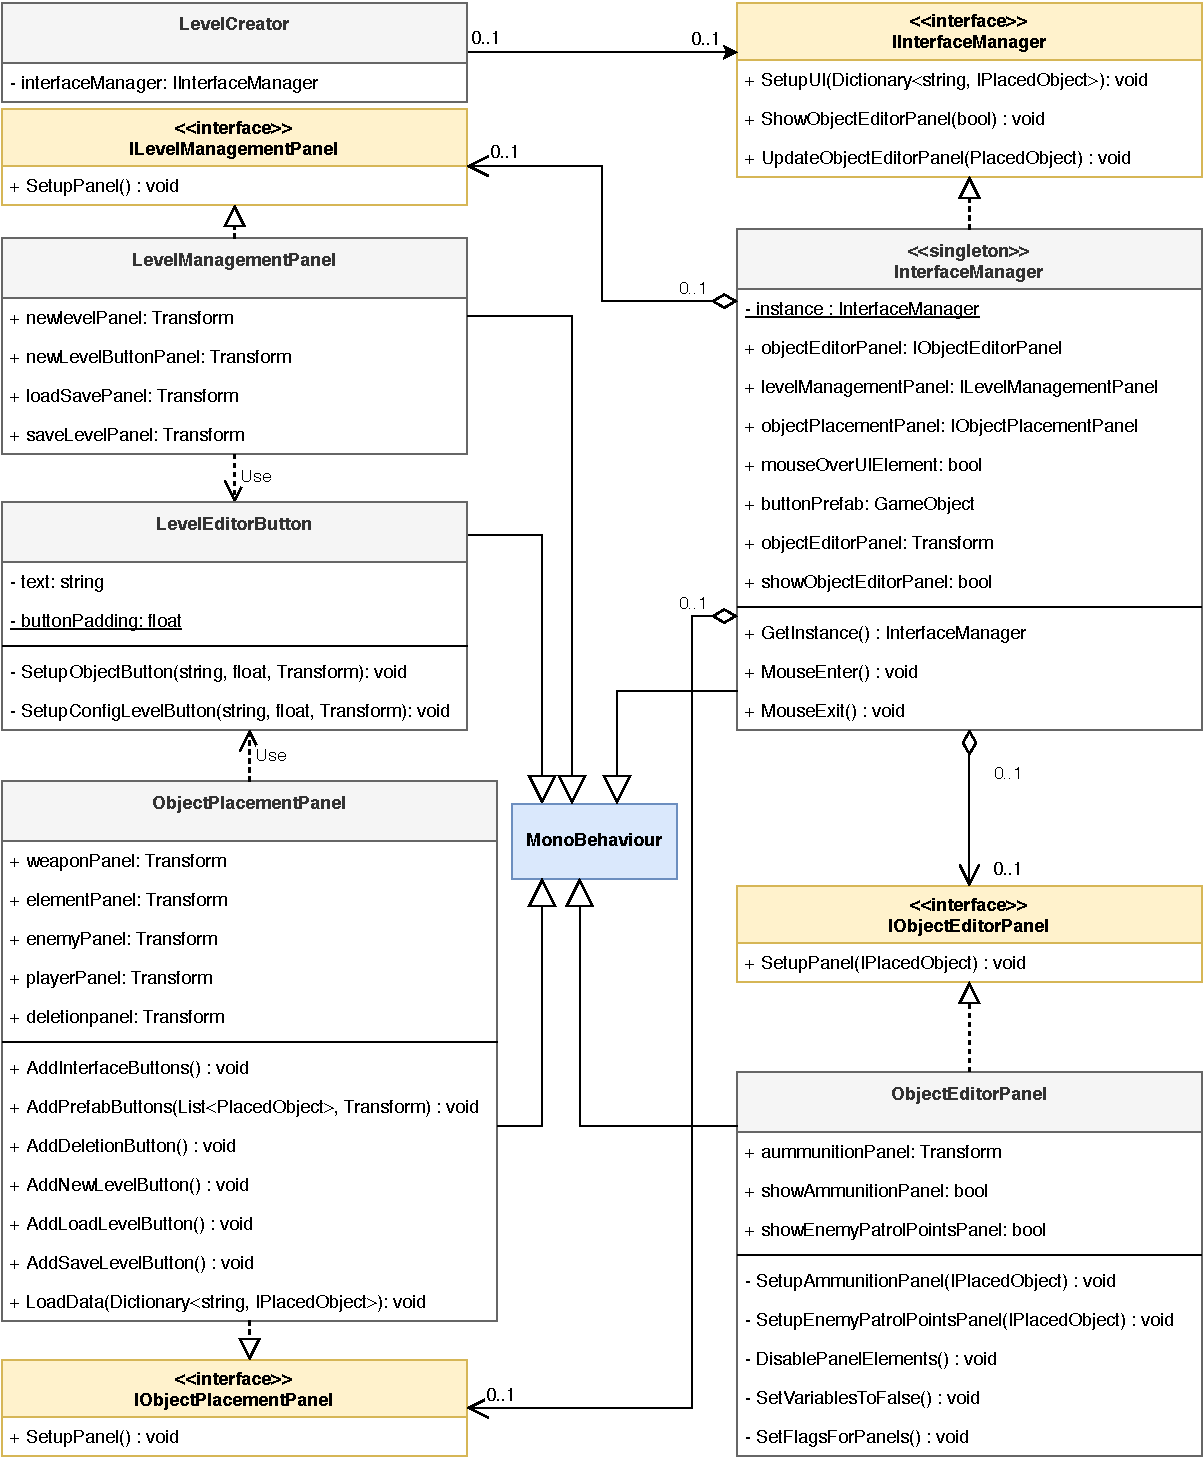
\includegraphics[width=1\textwidth]{pics/leveleditor_interfacemanager.pdf}
		\caption{Der \texttt{InterfaceManager}: Die Verwaltung der Benutzeroberfläche des Level-Editors}
		\label{fig:interfacemanager}
	\end {center}
\end {figure}

Mit Hilfe des \texttt{InterfaceManagers} wird die Benutzeroberfläche erstellt, aktualisiert und verschiedene Bereiche des Objekteditor-Bereiches der Benutzeroberfläche je nach Typ des im Editor ausgewählten \textit{Prefabs} angezeigt oder verborgen. Nach dem Laden der \textit{Prefabs} übergibt der \texttt{LevelCreator} die \textit{Prefabs}-Tabelle zum Auslesen an den \texttt{InterfaceManager}, um die Schaltflächen für alle platzierbaren Spielobjekte im Objekterstellungs- und Lösch-Bereich für die Benutzeroberfläche einzurichten. Dadurch kann bei Mausklick auf eine Schaltfläche später die hinterlegte ID des \textit{Prefabs} an den \texttt{PrefabsManager} übergeben werden, welcher eine neue Instanz des \textit{Prefabs} zum Platzieren übergibt. Abbildung \ref{fig:interfacemanager} zeigt die interne Implementierung des \texttt{InterfaceManagers}. Dieser ist intern in vier Bereiche unterteilt: Der \texttt{InterfaceManager} zur Gesamtverwaltung der Benutzeroberfläche und drei weitere eigenständige Komponenten für die im Kapitel Benutzeroberfläche vorgestellten Bereiche. 

Für die Interaktion des \texttt{LevelCreators} mit dem \texttt{InterfaceManager} werden die Funktionen \texttt{SetupUI(...)} zur Initialisierung der Benutzeroberfläche, die Funktion \texttt{ShowObjectEditor- \linebreak Panel(...)} zur Anzeige des Objekteditor-Bereiches, wenn sich der Editor im Zustand der Objektbearbeitung befindet, und die zugehörige Funktion \texttt{UpdateObjectEditorPanel(...)}. Mit dieser Funktion wird das auf der Karte ausgewählte Objekt übergeben und somit dem \texttt{InterfaceManager} alle Informationen zur Aktualisierung des Objekteditor-Bereiches übergeben. Für die Aktualisierung dieses Bereiches kümmert sich die Teilkomponente \texttt{ObjectEditorPanel}, an dem das dem \texttt{InterfaceManager} übergebene Objekt weitergereicht wird. Bei jeder Änderung der Textfelder, wird dieser Komponente das neue veränderte Objekt übergeben und aktualisiert den Objektbearbeitungs-Bereich. Die beiden anderen Bereiche, die Levelverwaltung und Objekterstellung und -löschung müssen nicht aktualisiert werden, da diese keine Felder zur Änderung des Zustandes eines Spielobjektes besitzen.

\begin {figure}[H]
	\begin {center}
	    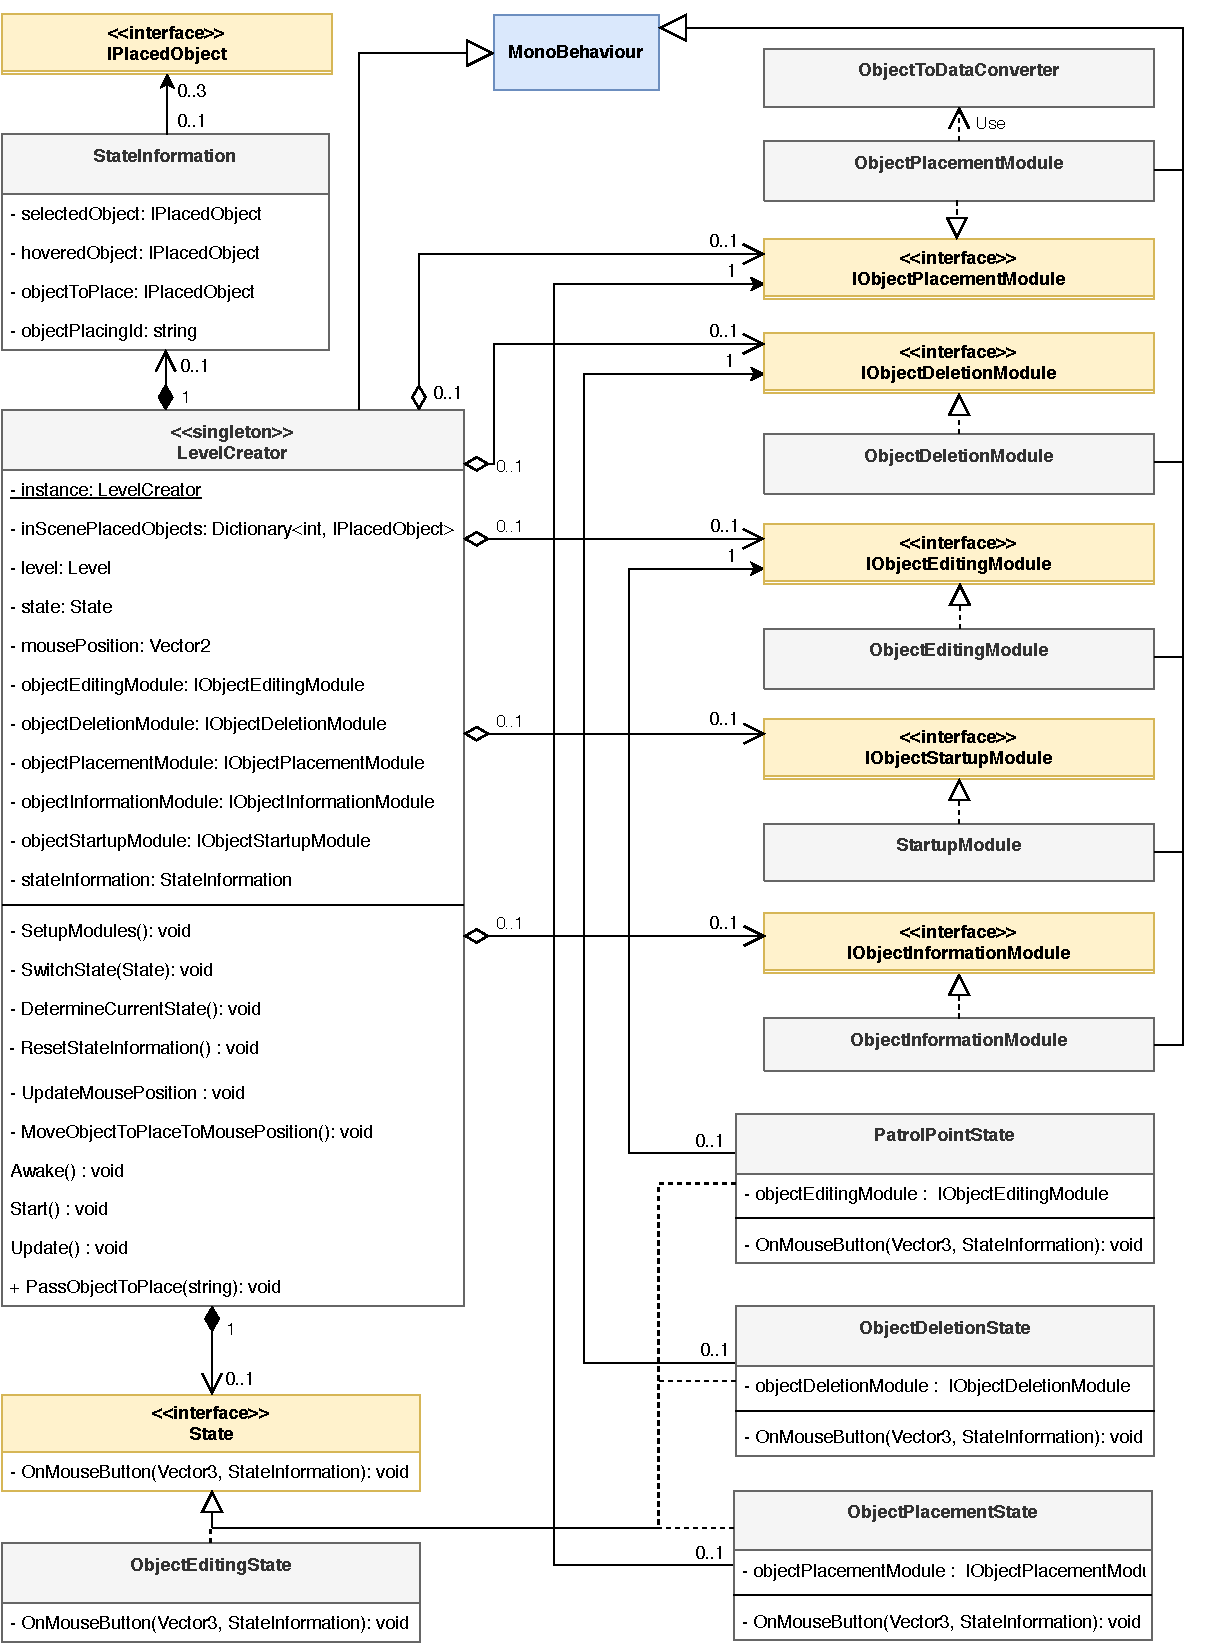
\includegraphics[width=1\textwidth]{pics/leveleditor_levelcreator_compressed.pdf}
		\caption{Der \texttt{LevelCreator}: Die Objektverwaltungskomponente im Level-Editor}
		\label{fig:leveleditor_levelcreator}
	\end {center}
\end {figure}

\subsubsection{Das Platzieren, Löschen und Editieren von 
von Spielobjekten}
Der \texttt{LevelCreator} stellt die Hauptkomponente des Level-Editors dar. Wie bereits erklärt

\begin{itemize}
	\item koordiniert diese Komponente die Initialisierung des Level-Editors und
	\item leitet Informationen an alle anderen Komponenten weiter.
	\item Die Annahme von Ereignissen, Weitergabe von Aufgaben an andere Komponenten und Koordination der Bearbeitung
\end{itemize}

Hierzu hat er selbst folgende wichtige Aufgaben:
\begin{itemize}
	\item Die Bestimmung des aktuellen Zustandes des Level-Editors
	\item Sicherstellung eines \glqq{}sauberen\grqq{} Zustandsüberganges
	\item Aktualisierung und Kontrolle der zu einem Zustand zugehörigen Zustandsinformationen
	\item Weitergabe von Aktionen wie dem Tastendruck der Maus an das aktuelle Zustandsobjekt über die Schnittstelle \texttt{State}
\end{itemize}

Wie bei der Benutzeroberfläche bereits erklärt wurde, gibt es die Zustände Objekterstellung, Objektlöschung, Objektbearbeitung und den Modus für das Setzen der Patroullienroute eines im Bearbeitungsmodus befindlichen Gegners. Ein Tastenklick mit der linken Maustaste kann dabei je nach Zustand eine andere Wirkung haben. Bei der Implementierung wurde daher das als \textit{State-Design-Pattern}\cite{Gamma.2011} bekannte Entwurfsmuster genutzt. Die für das Bearbeiten, Erstellen und Löschen eines Spiels notwendige Funktionalität lässt sich jedoch nur sehr schwer voneinander trennen, da diese Funktionalitäten oftmals voneinander stark abhängen. Beispielsweise werden im Platzierungsmodus alle Waffen und Gegner auf einem Levelstück gelöscht, wenn dort ein Levelelement platziert wird. Auf die zugehörige Funktionalität muss auch im Platzierungsmodus zugegriffen werden können. Um die Abhängigkeiten voneinander so gering wie möglich zu halten und eine Struktur hineinzubringen, wurde die gesamte Funktionalität in insgesamt 5 Module unterteilt und für den Zugriff auf jedes Modul, ein Interface implementiert. Abbildung \ref{fig:leveleditor_levelcreator} zeigt das entstandene Designkonzept für die Implementierung des \texttt{LevelCreators}. Aus Gründen der Übersichtlichkeit und aus Platzmangel mussten alle Methoden in den Modulen und zugehörigen Interfaces, sowie unwichtige Attribute in der Klasse \texttt{LevelCreator} weggelassen werden. 

Die Klasse \texttt{LevelCreator} kontrolliert den Zustand des Levels, während bei Aktionen je nach Zustand unterschiedliche Funktionalitäten vom jeweiligen Zustandsobjekt aufgerufen werden. Aktuell wird das Zustands-Entwurfsmuster nur für einen Tastendruck der linken Maustaste verwendet, dennoch ermöglicht dieses, das Verhalten des Level-Editors schnell anzupassen oder zu erweitern. Wie zu sehen, ist die eigentliche Funktionalität, dargestellt durch die Module, in die Bereiche Erstellen, Informationsausgabe, Editieren, Löschen, und Startup unterteilt. Diese Unterteilung wurde nach dem \textit{CRUD}-Prinzip\cite{Torim.2012} (Create, Read, Update, Delete) gewählt. Wie allgemein bekannt ist, können verschiedene Aktionen meist in die Bereiche Informationsausgabe (Read), Änderung (Update), Löschen (Delete) und Erstellen (Create) eindeutig eingeordnet werden. Der weitere Bereich Startup enthält Funktionalität, die ausschließlich zur Initialisierung eines Levels benötigt wird. Hierzu zählt beispielsweise das Setzen der äußeren Wände zur Randbegrenzung oder die Funktionalität zur Konvertierung der durch den \texttt{LevelController} geladenen Spielobjekte, die im nächsten Abschnitt genauer erläutert wird. 

Mit Hilfe der Methode \texttt{SwitchState()} wird der Zustand gewechselt. Dabei ist es auch möglich von einem Zustand wieder in den gleichen zu wechseln. Wird zum Beispiel im Objektbearbeitungsmodus auf ein anderes Objekt geklickt, so wird dieser Zustand beibehalten und die aktuellen Eigenschaften für das neu ausgewählte Objekt im Objektbearbeitungsbereich der Benutzeroberfläche angezeigt. Wird hingegen im Objektplatzierungsmodus auf die Schaltfläche für das bereits ausgewählte Objekt noch einmal gedrückt, so wird der Platzierungsmodus verlassen  und der Level-Editor befindet sich im Leermodus. Analog tritt dieser Fall ein, wenn im Löschmodus die Schaltfläche zum Aktivieren des Löschmodus gedrückt wird. Wechselt der Editor in den Leermodus, so wird immer die Methode \texttt{ResetStateInformation()} aufgerufen. Hierbei werden die im Zustandsinformations-Objekt gespeicherten Informationen gelöscht. In diesem Objekt werden die aktuell markierten, ausgewählten oder zu platzierenden Objekte, falls vorhanden, gespeichert. Mit Hilfe dieser Informationen kann im Objekt des aktuellen Zustandes die richtige Information entnommen und zur Bearbeitung an die Module weitergegeben werden. Dabei ist wichtig zu wissen, dass immer nur ein Zustand im Level-Editor gleichzeitig aktiv sein kann.
 

\subsubsection{Die Datenverwaltung und das Laden und Speichern eines Levels}
\begin {figure}[h]
	\begin {center}
	    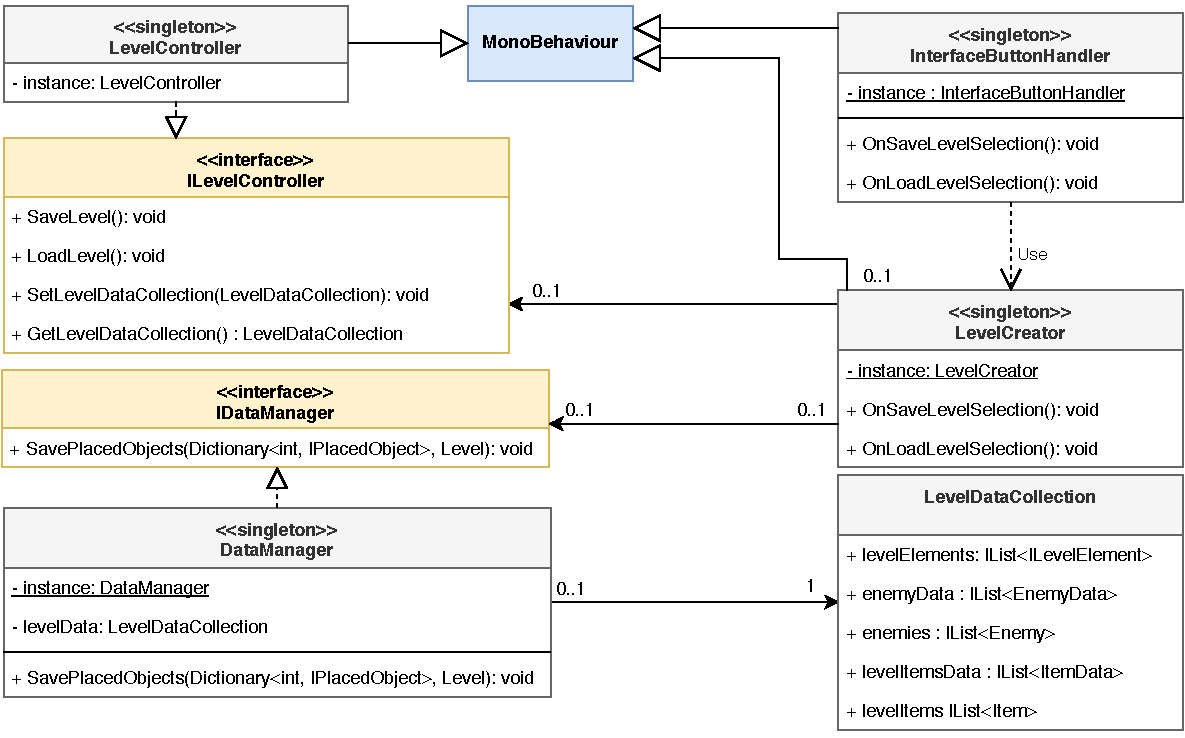
\includegraphics[width=1\textwidth]{pics/leveleditor_levelcontroller.pdf}
		\caption{Das Laden und Speichern mit Hilfe des \texttt{LevelControllers}}
		\label{fig:leveleditor_levelcontroller}
	\end {center}
\end {figure}

Für das Laden eines Levels zum Bearbeiten im Level-Editor oder das Speichern eines Levels im Editor kann bereits auf die Funktionalität zur Serialisierung und Deserialisierung im \texttt{LevelController} zurückgegriffen werden. Mit Hilfe dieser Komponente und der Datenverwaltungskomponente wird das Speichern und Laden eines Levels umgesetzt. Dabei wurde ein Interface eingeführt, um die Abhängigkeiten zwischen dem \texttt{LevelController} und dem \texttt{LevelCreator} so gering wie möglich zu halten.

Die Aufgabe der Datenverwaltung ist es die Daten zu den im Level befindlichen Spielobjekten zu verwalten, damit bei Speicherung des Levels alle für die Serialisierung notwendigen Informationen an den \texttt{LevelController }übergeben werden können. Diese eigenständigen Komponenten werden beim Speichern nacheinander ausgeführt, d.h. es werden die erstellten Informationen über die im Level befindlichen Spielobjekte von der Datenverwaltungskomponente über den \texttt{LevelCreator} an den \texttt{LevelController} über die Schnittstelle \texttt{ILevelController} übergeben. Dabei werden werden die Methoden \texttt{SetLevelDataCollection(...)} zur Aktualisierung der Referenzen auf die Daten und die Methode \texttt{SaveLevel()} aufgerufen, um den \texttt{LevelController} den Befehl zur Serialisierung und somit zur Speicherung des Levels zu geben. 

Für das Laden eines Levels wird zunächst die Methode \texttt{LoadLevel()} der Schnittstelle genutzt, um die Spielobjekte aus den gespeicherten Daten erstellen zu lassen. Nach dem Laden werden die im Objekt \texttt{LevelDataCollection} gespeicherten Referenzen zu diesen Spielobjekten vom \texttt{LevelCreator} über die Methode \texttt{GetLevelDataCollection()} des Interfaces geladen. Um diese Spielobjekte im Level-Editor bearbeiten zu können, ist es notwendig diese in das Format des Level-Editors zu übersetzen. Hierfür muss das \textit{Prefab} jedes Spielobjektes bestimmt und das zugehörige Container-Objekt im \texttt{PrefabsManager} geladen werden. Da die Eigenschaften des Spielobjektes des \textit{Prefabs} aus dem \texttt{PrefabsManager} wie die Position nicht mit den Eigenschaften des geladenen \textit{Prefabs} übereinstimmen, muss das im Container-Objekt untergeordnete Spielobjekt gegen das geladene Spielobjekt ersetzt werden. Danach werden die Position auf das Container-Objekt übertragen, bestimmte Komponenten des Spielobjektes deaktiviert und der \textit{Collider} des jeweiligen Spielobjektes auf das Container-Objekt übertragen.

\pagebreak

% Testen des Spiels
\section{Softwaretests in Verbindung mit Unity}
\label{sec:testing}

In den vorhergehenden Kapiteln wurden die verschiedenen Funktionalitäten des Spiels ausführ\-lich beschrieben. Um das Vertrauen in die eigene Arbeit zu erhöhen und Fehler im Zuge des Entwicklungsprozesses frühzeitig identifizieren zu können, ist die Erstellung und Durchführung von Softwaretests ein weiterer wichtiger Bestandteil des Projekts. 

%Bei der Entwicklung von Software ist Testen aus vielerlei Gründen eine wichtige Aufgabe. Unter anderem wird hierdurch das Vertrauen in die eigene Arbeit erhöht, da fehleranfällige Stellen zu einem frühen Zeitpunkt im Entwicklungsprozess identifiziert werden. Des Weiteren wird in vielen Projekten ein gewisser Erfüllungsgrad verschiedenster Testmetriken vonseiten der Auftraggeber gefordert, um das Vertrauen in das entwickelte Produkt auch auf Gegenseite herzustellen. 

Im Folgenden wird die Durchführung von zweierlei Arten von Tests beschrieben, die bei der Entwicklung des Projekts zum Einsatz kommen. Zunächst wird hierbei auf automatisierte Modultests inklusive deren Besonderheiten in Verbindung mit dem Unity Framework eingegangen. Anschließend werden verschiedene manuelle Tests vorgestellt, die im Zuge des Projekts durchgeführt werden.  

\subsection{Modultests}

Um die einwandfreie Funktionalität des implementierten Quellcodes bereits zur Entwicklungszeit
sicherstellen zu können, wurden automatisierte Modultests parallel zum eigentlichen
Programmcode entwickelt. Die Verwendung des Unity Frameworks erforderte hierbei ein vom Standard abweichendes Vorgehen, welches im Nachfolgenden näher erläutert wird. Hierbei wird zunächst auf die allgemeine Vorgehensweise zur Erstellung von Modultests unter Unity eingegangen. Anschließend werden Problemstellungen erläutert, die sich daraus ergeben, und zwei Lösungsansätze dafür aufgezeigt. Abschließend wird eine Übersicht bezüglich der Testabdeckung innerhalb des Projekts gegeben. 

\subsubsection{Allgemeines zu Modultests in Unity}

%https://de.slideshare.net/MikkoMcMenamin/unit-testing-in-unity-128173223


Das Unity Framework unterstützt Entwickler bei der Erstellung von Modultests durch die Bereitstellung einer Test Applikation, dem \textit{Unity Test Runner} (siehe Abb. \ref{fig:unity_test_runner}). Dieser ist ein grafisches Werkzeug, das die Ausführung von Testfällen per Knopfdruck ermöglicht und eine visuelle Rückmeldung bezüglich der einzelnen Ergebnisse liefert. 

%\vspace{1em}
%\begin{minipage}{\linewidth}
%	\begin{center}
      \begin{figure}[!t]
      \begin{center}
		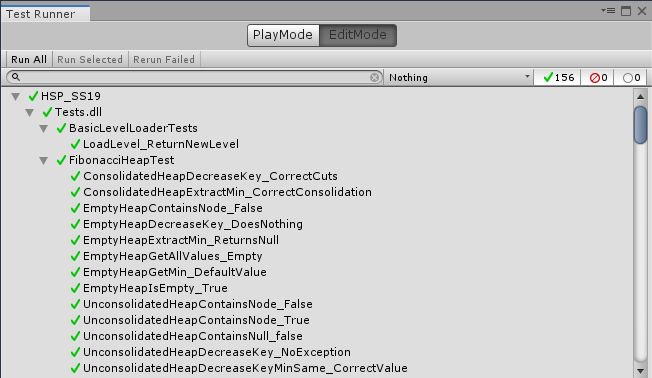
\includegraphics[width=1.00\linewidth]{pics/unity_test_runner.png}
		\captionof{figure}[Grafische Oberfläche des Unity Test Runners]{Grafische Oberfläche des Unity Test Runners}
		\label{fig:unity_test_runner}
		  \end{center}
		\end{figure}
%	\end{center}
%\end{minipage}

Wie in Abbildung \ref{fig:unity_test_runner} zu erkennen ist, können Testfälle in die beiden Kategorien \textit{PlayMode} und \textit{EditMode} unterteilt werden. Die Zuordnung erfolgt durch eine entsprechende Annotation über der Signatur einer Testmethode. Modultests, die als \textit{EditMode} deklariert sind, stellen die leichtgewichtigere Variante dar. Diese Testmethoden entsprechen dem auch außerhalb von Unity üblichen Verständnis von Modultests. Bei der Ausführung der Tests werden diese direkt im Editor-Modus von Unity durchgeführt. Spezielle Methoden von Spielobjekten, wie beispielsweise \texttt{Update()}, \texttt{Awake()} und \texttt{Start()} werden hierbei nicht aufgerufen. Tests, die im \textit{EditMode} ausgeführt werden, benötigen daher wenig Zeit zur Durchführung und sind äußerst performant. Ihr Einsatz zielt in erster Linie auf die Überprüfung einzelner isolierter Methoden ab, die ein gleichbleibendes Verhalten aufweisen und nicht von mehreren aufeinanderfolgenden Einzelbildern oder der Unity Spieleengine abhängen. Ein Beispiel hierfür ist die Funktionalität einer Datenstruktur. Im Gegensatz hierzu wird bei jeder als \textit{PlayMode} Test deklarierten Methode eine komplette Spielszene innerhalb der Unity-Engine geladen und alle oben genannten Methoden werden für jedes Spielobjekt ausgeführt. Das System verhält sich bei der Ausführung eines \textit{PlayMode} Tests exakt so, als würde ein Benutzer die Unity Applikation starten und die jeweilige Methode ausführen. Dies resultiert in lang andauernden Prozessen, die eher zur Überprüfung dynamischer Spielinhalte über mehrere Einzelbilder hinweg oder auch zur Überprüfung bestimmter Eigenschaften erzeugter Spielobjekte geeignet sind. Durch \textit{PlayMode} Tests lassen sich beispielsweise Testfälle konstruieren, die die Bewegung eines Spielobjekts über den Bildschirm verfolgen und innerhalb eines jeden Einzelbilds die tatsächliche Position des Objekts mit der kalkulierten, erwarteten Position vergleichen. Die Einsatzbereiche der beiden Varianten von Modultests sind nicht klar abgegrenzt. Die Vor- und Nachteile müssen für jede Funktionalität gegenübergestellt und auf ihre Verwendbarkeit hin untersucht werden.  

%- Play Mode: Unity Engine wird gesteartet
%- Play Mode: Auch hier können keine MonoBehaviours instanziiert werden. Entweder leeres Spielobjekt usw. , oder ganze Szene laden!
%- Play Mode: Möglichkeit 2: Ganze Szene wird geladen! Mit allen !!!Spielobjekten, etc. => Keine isolierten Tests von kleinen Komponenten! Modultests => kleinste Module => Methoden!
%
%- PlayMode Tests testen ganze Abläufe, sind sehr langsam. 




Zur Implementierung der Modultests wird die Open-Source Bibliothek NUnit\footnote{https://nunit.org/} verwendet. Durch Annotation der Methoden innerhalb einer Testklasse lassen sich diese Methoden in unterschiedliche Kategorien mit verschiedenen Verwendungszwecken einteilen. In Tabelle \ref{tab:nunit_annotations} sind die wichtigsten Annotationen der NUnit Bibliothek mit ihren zugehörigen Bedeutungen beschrieben. Des Weiteren bietet NUnit vielfältige Möglichkeiten in Form von statischen Methoden, um erwartete mit tatsächlichen Ergebnissen zu vergleichen oder auch bestimmte Eigenschaften von Resultaten zu überprüfen. 

%- Wichtige Annotationen


\begin{table}[t!]
\caption[Häufig genutzte Annotationen der NUnit Bibliothek mit zugehöriger Bedeutung]{Häufig genutzte Annotationen der NUnit Bibliothek mit zugehöriger Bedeutung}
\begin{center}
\begin{tabular}{|l|l|}
\hline
  Annotation & Beschreibung \\
  \hline
  \texttt{$[$Test$]$} & Kennzeichnet eine Methode innerhalb einer Testklasse als Test. \\
  \texttt{$[$TestCase$]$} & Ermöglicht die mehrmalige Ausführung einer Testmethode mit \\ 
  &	verschiedenen Argumenten. \\
  \texttt{$[$SetUp$]$} & Kennzeichnet eine Methode, die \textbf{vor jedem} Test einer Testklasse \\
  & aufgerufen wird. \\
  \texttt{$[$TearDown$]$} & Kennzeichnet eine Methode, die \textbf{nach jedem} Test einer Testklasse \\
  & aufgerufen wird.  \\
  \texttt{$[$OneTimeSetUp$]$} & Kennzeichnet eine Methode, die \textbf{einmalig vor allen} Tests einer \\
  & Testklasse ausgeführt wird. \\ 
  \texttt{$[$OneTimeTearDown$]$} & Kennzeichnet eine Methode, die \textbf{einmalig nach allen} Tests einer \\
  & Testklasse ausgeführt wird.  \\
  \hline
\end{tabular}
\label{tab:nunit_annotations}
\end{center}
\end{table}

%=>> Wichtige Methoden (Assert, etc.) ???

Bei der Erstellung von Modultests muss berücksichtigt werden, dass viele zu testende Module aufgrund von äußeren Abhängigkeiten nicht beziehungsweise nur schwer isoliert getestet werden können. Diese Abhängigkeiten können beispielsweise Eingabeparameter sein, die über spezielle Eigenschaften verfügen, welche dann in einer konkreten Testmethode zur Steuerung des Kontrollflusses verwendet werden. Um eine funktionale Komponente so isoliert wie nur möglich testen zu können, muss daher in vielen Fällen die Umgebung der zu testenden Funktionalität künstlich nachgebildet werden. Dies geschieht durch die Verwendung von Platzhalter-Objekten, auch \textit{Mocks} genannt, die anstelle von realen Instanzen der notwendigen Klassen verwendet werden. In diesem Projekt wird hierfür die Bibliothek NSubsitute\footnote{https://nsubstitute.github.io/} verwendet. 

Ein weitverbreitetes Vorgehen bei der Erstellung von Modultests ist die Strukturierung der inneren Funktionalität einer Testmethode in drei klar voneinander abgegrenzte Bereiche. Diese Bereiche werden als \textit{Vorbereitung}, \textit{Aktion} und \textit{Bestätigung} bezeichnet. Im ersten Abschnitt werden alle Objekte, die für den Aufruf der zu testenden Methode notwendig sind, initialisiert und die Werte der Daten festgelegt, die an die zu testende Methode übergeben werden. Anschließend wird die zu testende Methode mit den vorbereiteten Daten aufgerufen. Im dritten Bereich wird überprüft, ob das Ergebnis der zu testenden Methode mit dem erwarteten Ergebnis übereinstimmt. Dieses Vorgehen wird, in Anlehnung an die Anfangsbuchstaben der englischen Bezeichnungen der einzelnen Bereiche \textit{Arrange}, \textit{Act} und \textit{Assert}, auch als \textit{AAA}-Muster bezeichnet. Auch in diesem Projekt werden die Testmethoden nach dieser Struktur entwickelt. 

%\begin{tabular}[t]{ll}
%%\tabitem 
%\textbf{Wand:} & Position\\
%\textbf{Tür:} & Position, Rotation\\
%\textbf{Waffe:} & Position, Rotation, Typ, Munitionsmenge\\
%\textbf{Gegner:} & Position, Typ, Patrouillenpunkte, Waffentyp, Munitionsmenge\\
%\textbf{Ziel:} & Position\\
%\textbf{Level:} & Größe, Startposition, Aktuelle Position
%\end{tabular}


\subsubsection{Schwierigkeiten bei der Erstellung der Modultests}

Die Entwicklung von Modultests in Unity Projekten ist mit verschiedenen Herausforderungen verbunden, die in Projekten außerhalb der Unity-Engine nicht existieren. Diese resultieren aus dem von Unity festgelegten Zusammenspiel zwischen Spielobjekten, Verhaltensklassen, die diesen Spielobjekten als Komponenten hinzugefügt werden können, und den logischen Abhängigkeiten innerhalb dieser Klassen.

Die größte Herausforderung stellt hierbei das Testen von Klassen dar, die von der Unity eigenen Basisklasse \textit{MonoBehaviour} erben. Da jede Klasse, die einem Spielobjekt als Komponente hinzugefügt werden soll, von \textit{MonoBehaviour} erben muss, ist die Zahl dieser abgeleiteten Klassen innerhalb eines Unity Projekts sehr groß. 

Dies bringt verschiedene Probleme mit sich. Zum einen lassen sich von \textit{MonoBehaviour} abgeleitete Klassen nicht auf Ebene des Quellcodes instanziieren. Dies ist allerdings eine Grundvoraussetzung, um im Aktionsbereich eines Modultests eine zu testende Methode dieser Klasse aufrufen zu können. Zum anderen können Klassen dieses Typs auch nicht durch Platzhalter Objekte nachgebildet werden. Dies hat zur Konsequenz, dass die Umgebungen von Klassen, die selbst zwar nicht von \textit{MonoBehaviour} erben, aber Abhängigkeiten zu solchen abgeleiteten Klassen besitzen, nur sehr schwer und stellenweise unmöglich nachzustellen sind.

Die Tatsache, dass von \textit{MonoBehaviour} abgeleitete Klassen nicht instanziiert werden können, bringt auch weiterführende Probleme in Hinblick auf statistische Aspekte im Zuge der Qualitätssicherung mit sich. Herkömmliche Werkzeuge zur Überprüfung der Testabdeckung und Ermittlung verschiedener Testmaße lassen sich nicht mehr ohne Weiteres benutzen, da die implementierten Testmethoden vom Standard abweichend entwickelt werden müssen, um ausgeführt werden zu können. 

Eine weitere Herausforderung im Zuge des Entwicklungsprozesses ist die Durchführung von \textit{PlayMode} Testfällen. Da zu Beginn eines jeden Testfalls eine komplette Spielszene innerhalb der Unity-Engine geladen wird, ist die Ausführung dieser Tests sehr rechen- und zeitintensiv. Bereits wenige Testfälle genügen, um eine länger andauernde Testphase zu verursachen. Mit steigender Anzahl an Testfällen nimmt die benötigte Zeit schnell zu, wodurch eine iterative Durchführung im laufenden Entwicklungsprozess erschwert wird. 

%- Klassen, die von MonoBehaviour erben -> Wieso sind die ein Problem? -> Begründung! (Kann man nicht instanziieren, ...) => WARNUNG, kein ERROR!
%
%- Kann man nicht mit NSubstitute mocken!
%
%- Warum nicht Play Mode Tests: jedes Mal wird die ganze Unity Engine gestartet! => Im laufenden Entwicklungsprozess zu aufwändig für jede kleine Komponente!
%
%- Testabdeckung mit herkömmlichen Tools nicht möglich

\subsubsection{Beschreibung verschiedener Lösungsansätze zum Testen von MonoBehaviours}
\label{chapter:mono_beh_testen_loesungen}

Es existieren zwei unterschiedliche Ansätze, um von \textit{MonoBehaviour} abgeleitete Klassen zu testen. Bei ersterer Möglichkeit werden einer Testklasse zwei private Attribute hinzugefügt, wobei ein Attribut vom Typ \texttt{GameObject} und das andere vom Typ der Klasse sein muss, deren Funktionalität überprüft werden soll. Anschließend wird ein neues \texttt{GameObject} instanziiert und die Referenz dem entsprechenden Attribut zugewiesen. Dem neu erstellten, leeren Spielobjekt wird nun die Klasse mit der zu testenden Funktionalität als Komponente hinzugefügt. Der Rückgabewert dieser Methode wird in dem dazugehörigen Attribut abgespeichert. Ab diesem Zeitpunkt ist es möglich, alle öffentlichen Methoden der Klasse aufzurufen, welche die zu testende Funktionalität enthält. Da das soeben beschriebene Vorgehen zu Beginn einer jeden Testmethode ausgeführt werden muss, bietet es sich an, den hierfür notwendigen Programmcode in eine eigene Methode auszulagern und diese mit der NUnit Annotation \texttt{OneTimeSetUp} zu kennzeichnen. Die Methode wird hierdurch einmalig zu Beginn der Testphase ausgeführt und die gesetzten, privaten Attribute können in allen folgenden Testmethoden verwendet werden. 

Eine weitere Möglichkeit zur Lösung des Problems ist die Anwendung des \textit{Humble Object Pattern} \cite{xUnit_Test_Patterns_Refactoring}. Gerard Meszaros beschreibt in seinem Lehrbuch sieben unterschiedliche Varianten dieses Entwurfsmusters, die sich je nach konkretem Anwendungsfall unterscheiden. Im Folgenden wird lediglich die für das Projekt relevante Variante näher beschrieben, für eine ausführliche Erläuterung der übrigen Optionen siehe \cite{xUnit_Test_Patterns_Refactoring}.

Die grundlegende Idee des Entwurfsmusters ist es, den Programmcode, der die eigentliche Logik ausführt, in eine neue Komponente auszulagern und diese isoliert zu testen. Eine Visualisierung dieser Vorgehensweise ist in Abbildung  \ref{fig:humble_object_pattern} dargestellt. Anstatt die zu testende Komponente mit ihren Abhängigkeiten direkt zu testen (Abb. \ref{fig:humble_01}) wird die relevante Logik in eine neue Komponente verlagert und dort getestet (Abb. \ref{fig:humble_02}). Das \textit{Humble Objekt} agiert dann nur noch als eine Art Vermittlerschicht, die die isolierte Funktionalität dieser Komponente aufruft und die Rückgabewerte weiterverarbeitet. Innerhalb des \textit{Humble Objekts} wird wenig eigener Quellcode benötigt. Es ist lediglich für die Bereitstellung der benötigten Informationen beim Aufruf der ausgelagerten Methoden verantwortlich. Da der übrige Quellcode innerhalb eines \textit{Humble Objekts} vor allem die Interaktion des Objekts mit seiner Umwelt zum Ziel hat, kann auf das Testen dieser Funktionalitäten meist verzichtet werden. 


      \begin{figure}[tbh]
      \centering
      \begin{minipage}[c]{0.8\textwidth}
     \subfloat[\label{fig:humble_01}]{
       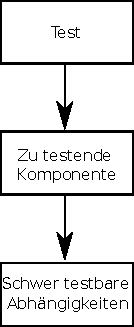
\includegraphics[width=0.2205\textwidth]{pics/humble_object_pattern_01.pdf}
     }
     \hfill
     \subfloat[\label{fig:humble_02}]{
       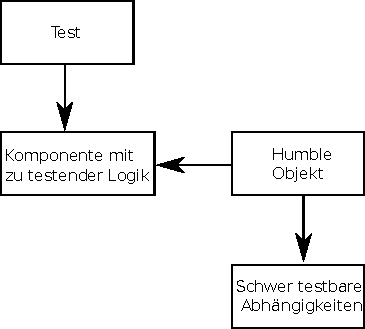
\includegraphics[width=0.598\textwidth]{pics/humble_object_pattern_02.pdf}
     }
     \hfill
     \caption[Veranschaulichung des \textit{Humble Object Pattern}.]{Veranschaulichung des Humble Object Pattern. Abbildung \sref{fig:humble_01} zeigt die Ausgangssituation, in \sref{fig:humble_02} wird das Ergebnis dargestellt. Die tatsächliche Logik einer Komponente wird in eine neue Klasse ausgelagert und dort isoliert getestet.}
     \label{fig:humble_object_pattern}
\end{minipage}
   \end{figure}


In \cite{xUnit_Test_Patterns_Refactoring} beschreibt Meszaros drei verschiedene Möglichkeiten, die Referenz eines \textit{Humble Objekts} auf die Komponente, die die ausgelagerte Logik enthält, zu realisieren. Die simpelste Möglichkeit ist, für jede Methode einer Klasse eine weitere Methode zu erstellen, die die tatsächliche Logik enthält. Hierbei ist keine Referenz zu anderen Klassen notwendig, allerdings leidet die Übersichtlichkeit und Klassen können schnell sehr groß werden. Bei Variante zwei wird für jede Klasse, die zu testende Funktionalität enthält, eine neue Klasse erstellt und die zu testenden Methoden mit der tatsächlichen Logik innerhalb dieser platziert. Das \textit{Humble Objekt} hält dann eine Referenz auf diese Klasse. Die letzte Möglichkeit erweitert dieses Vorgehen noch und sieht vor, das \textit{Humble Objekt} als abgeleitete Klasse der Klassen mit ausgelagerter Funktionalität zu realisieren. Somit können die Methoden mit ausgelagerter Funktionalität in verschiedenen Klassen verwaltet werden. Das \textit{Humble Objekt} muss lediglich von diesen Klassen erben und keine Referenzen speichern.

Hinsichtlich des konkreten Projekts ergeben sich durch eine Gegenüberstellung der beiden soeben vorgestellten Herangehensweisen Vor- und Nachteile für beide Seiten. Das Hinzufügen einer Komponente zu einem leeren Spielobjekt führt zu weniger Klassen, als es bei der Anwendung des \textit{Humble Object Pattern} der Fall wäre. Dort wird für jede zu testende Klasse eine weitere benötigt, wodurch sich die Anzahl notwendiger Klassen verdoppelt. Dies resultiert in unübersichtlicheren Strukturen. Darüber hinaus ist es oftmals nicht ohne Weiteres möglich, anwendungsbezogenen Quellcode von äußeren Abhängigkeiten klar abzugrenzen. Die Auslagerung der für die Logik verantwortlichen Codefragmente in eigene Methoden erfordert in manchen Fällen einen nicht unerheblichen Aufwand und führt auch hier zu unübersichtlicheren Strukturen mit stellenweise viel Quellcode, der lediglich die Kommunikation zwischen dem \textit{Humble Objekt} und dem ausgelagerten Code steuert. Diese Kommunikation führt neben einem höheren Entwicklungsaufwand auch zu Einbußen hinsichtlich der Performanz des Gesamtsystems. Ein positiver Aspekt des \textit{Humble Object Pattern} ist die Tatsache, dass mit Hilfe von Standardverfahren und Werkzeugen verschiedene Testüberdeckungsmetriken berechnet werden können. Doch selbst dieses Argument wird durch Unity eigene Besonderheiten abgeschwächt, die eine automatisierte Auswertung der Testüberdeckung erschweren. Nach Abwägung aller Vor- und Nachteile wurde daher entschieden, die zu testenden Komponenten direkt zu testen und daraus entstehende Nachteile bewusst in Kauf zu nehmen. 


%- Direkt die Klassen testen (wie kommt man mit MonoBehaviours klar?) => Leere Spielobjekte erstellen und Komponenten hinzufügen. 
% - Schneller!
%- Keine redundanten Klassen
%- Weniger Codevolumen
%- Übersichtlicherer Code
%- Teilweise sehr kompliziert, den Code auszulagern (Abhängigkeiten, siehe Zugriff auf transform-Objekte usw. ...)
%- 
%\linebreak
%- Funktionalen Code auslagern in extra Klassen -> \textit{Humble Object Pattern} [Vgl. \cite{xUnit_Test_Patterns_Refactoring}]
%
%- Metriken zur Code-Coverage einfacher möglich
%- 



%\subsubsection{Gewähltes Vorgehen und Begründung}
%Evtl ganz rauswerfen. Steht alles schon im vorhergehenden Kapitel. 

%
%\subsubsection{Unlösbare Probleme und mögliche Alternativen}
%
%- Serialisierung automatisiert testen. -> Es werden LevelElemente serialisiert, und diese existieren nicht wenn die Unity Engine nicht läuft (also im isolierten automatischen Test)! Diese lassen sich auch nicht im Testfall erzeugen, da es MonoBehaviours sind! Deserialisieren und dann serialisieren funktioniert auch nicht, da beim Deserialisieren nur LevelElementDATA Objekte deserialisiert/wiederhergestellt werden, und diese dann mithilfe der Unity Engine (die beim isolierten Test nicht vorhanden ist) in LevelElemente umgewandelt werden! Gleiches Problem -> die LevelElementDATA Objekte können nicht in LevelElements überführt werden, die aber zur Serialisierung notwendig sind!
%
%- LevelController, ...

%\subsubsection{Ausgewählte Problemstellungen}

\subsubsection{Übersicht bezüglich der Testabdeckung}

\begin{table}[b!]
\caption[abc]{Darstellung verschiedener Eigenschaften sowie selbst definierter Metriken für verschiedene Komponenten des Projekts.}
\begin{center}
\begin{tabular}{|l||l|l|l|l|l||l|l|}
\hline
  Funktionalität & Klassen $k$ & Methoden $m$ & $LOC_F$ & Testfälle $t$ & $LOC_T$ & $\frac{t}{m}$ & $\frac{LOC_T}{LOC_F}$ \\
  \hline
  Audio & 11 & 21 & 437 & 0 & 0 & 0,00 & 0,00 \\
  Kamera & 1 & 1 & 47 & 0 & 0 & 0,00 & 0,00 \\
  Anzeige & 3 & 0 & 131 & 0 & 0 & 0,00 & 0,00 \\
  Hauptmenü & 4 & 11 & 162 & 0 & 0 & 0,00 & 0,00\\
  Spielersteuerung & 2 & 11 & 284 & 0 & 0 & 0,00 & 0,00\\
  Level Elemente & 9 & 15 & 419 & 20 & 289 & 1,33 & 0,69 \\
  Levelaufbau & 10 & 40 & 910 & 60 & 1.047 & 1,68 & 1,50\\
  Level-Editor & 10 & 37 & 1.282 & 0 & 0 & 0,00 & 0,00\\
  Level speichern/ &&&&&&&\\
  Level laden & 3 & 6 & 448 & 4 & 760 & 0,67 & 1,70\\
  Waffen & 10 & 16 & 468 & 0 & 0 & 0,00 & 0,00\\
  Gegner und &&&&&&&\\
  KI Verhalten & 11 & 34 & 1.089 & 0 & 0 & 0,00 & 0,00\\
  KI Schnittstelle & 4 & 13 & 551 & 0 & 0 & 0,00 & 0,00\\
  Pfadfindung & 10 & 12 & 623 & 12 & 346 & 1,00 & \\
  Fibonacci-Heap & 2 & 12 & 215 & 20 & 379 & 1,67 & 1,76\\  
  Hilfsklassen & 4 & 14 & 238 & 40 & 237 & 2,86 & 1,00\\  
  \hline
\end{tabular}
\label{tab:testabdeckung}
\end{center}
\end{table}

Wie bereits in Kapitel \ref{chapter:mono_beh_testen_loesungen} beschrieben, erschwert das gewählte Vorgehen zur Entwicklung der Modultests die automatisierte Auswertung hinsichtlich verschiedener Metriken. Es wurden daher eigene Maße definiert, um eine Aussage bezüglich der Testabdeckung innerhalb der verschiedenen Komponenten des Projekts zu erhalten und diese untereinander vergleichen zu können. Die manuelle Auswertung dieser Maße ist in Tabelle \ref{tab:testabdeckung} dargestellt. In Spalte eins sind die verschiedenen Komponenten aufgeführt. Hierzu werden Klassen mit identischen Einsatzbereichen zu Oberkategorien zusammengefasst. Die Spalten zwei, drei und vier geben Auskunft über die Anzahl Klassen, Anzahl Methoden und Anzahl geschriebener Zeilen Quellcode innerhalb dieser Komponenten. In Spalte drei werden lediglich öffentlich zugreifbare Methoden berücksichtigt, da Implementierungsdetails innerhalb privater Methoden für den Benutzer einer Klasse nicht relevant sind. Da die nachfolgende Spalte einen Überblick hinsichtlich des Codevolumens innerhalb einer Komponente gibt, werden hierbei wiederum alle Funktionalitäten jeglicher Zugriffsmodifikatoren berücksichtigt. In den folgenden beiden Spalten werden die Anzahl Testfälle sowie die Anzahl geschriebener Zeilen Quellcode innerhalb dieser Testfälle aufgelistet. Parametrisierte Tests, also Testmethoden gleicher Struktur, die mit unterschiedlichen Argumenten aufgerufen werden, werden sowohl bei der Bestimmung der Anzahl Testfälle als auch in Bezug auf den Umfang des Quellcodes als separate Tests betrachtet. Die letzten zwei Spalten zeigen selbst definierte Metriken, die zum einen das Verhältnis existierender Testfälle zu vorhandenen öffentlichen Methoden und zum andern den Quotienten aus der Anzahl Zeilen zur Erstellung der Testfälle und Anzahl Zeilen der tatsächlichen Funktionalitäten wiedergeben. 

Hierbei ist zu erkennen, dass für nur fünf von möglichen fünfzehn Komponenten überhaupt Testfälle existieren. Dies lässt sich durch die Bedeutung dieser Komponenten im Projekt erklären. Die Kategorien Level Elemente, Levelaufbau, Level speichern und Level laden, Pfadfindung und Fibonacci-Heap stellen Grundfunktionalitäten der Software dar, auf denen viele andere wichtige Entwicklungen aufbauen. Die im Verhältnis meisten Testfälle pro öffentlicher Methode sind in den Hilfsklassen zu finden. Der Grund hierfür ist die Verwendung vieler parametrisierter Tests, deren primäres Ziel die Überprüfung der zu testenden Methoden mit unterschiedlichen Argumenten darstellt. Das Verhältnis von geschriebenen Zeilen Testcode zur Anzahl funktionaler Zeilen ist bei der Fibonacci-Heap Datenstruktur am höchsten. Aufgrund des relativ geringen Umfangs der tatsächlichen Funktionalität genügen hierzu vergleichsweise unterdurchschnittlich viele Zeilen Testcode. 





% Die Aussagekraft der in Tabelle \ref{tab:testabdeckung} dargestellten Zahlen muss allerdings auch

%- Unity hat test coverage tool eingestellt usw. 




%- Testabdeckung (Automatisiert nicht möglich, Gründe, Vom Markt genommen, ...)
%- Offizielles Statement von Unity zu Testabdeckung/Testen
%- Was konnte denn getestet werden, was nicht? Welche Klassen sind ganz gut abgedeckt, welche überhaupt nicht? Gründe dafür nennen!

\subsection{Manuelle Tests}

Neben automatisierten Modultests ist auch die Durchführung manueller Tests ein wichtiger Bestandteil des Projekts. Dies ist zum einen in Szenarien notwendig, in denen automatisierte Tests aufgrund vieler komplexer Abhängigkeiten nur schwer erstellbar sind. Zum anderen eignen sich manuelle Tests zur Überprüfung von Spielabläufen, in denen das Zusammenspiel mehrerer Komponenten miteinander untersucht werden muss. Da die manuelle Begutachtung sehr schnell und unkompliziert ausgeführt werden kann, stellt dieses Vorgehen eine echte Alternative zum Schreiben von \textit{PlayMode} Tests dar. Im Folgenden sind die wichtigsten Funktionalitäten stichpunktartig aufgeführt, deren korrektes Verhalten durch manuelle Tests überprüft wurde: 

\begin{itemize}
\item Steuerung des Spielers: Der Spieler bewegt sich entsprechend der getätigten Eingaben und kann nicht durch Wände hindurchgehen. Das Ablegen und Aufheben von Waffen sowie das Sammeln von Munition funktioniert wie erwartet. Ein Spieler kann nicht durch geschlossene Türen oder Wände hindurchschießen.  
\item Level speichern und laden: Ein aktueller Spielstand kann per Knopfdruck auf zweierlei Arten gesichert und zu einem späteren Zeitpunkt über das Hauptmenü korrekt wiederhergestellt werden. 
\item Gegnerverhalten, Pfadfindung und Audio: Gegner reagieren auf Geräusche in ihrer Umgebung sowie auf Sichtkontakt mit dem Spieler. Des Weiteren verfolgen Gegner den Spieler, allerdings sind diese nicht allwissend und brechen die Verfolgung bei gewissen Bedingungen wieder ab. Anschließend kehren sie zu ihrer ursprünglichen Route zurück. 
\item Level-Editor: Verschiedene Level Elemente (Wände, Türen) sowie Waffen können frei platziert werden. Die Größe eines Levels kann beliebig festgelegt werden. Ein erstelltes Level kann gespeichert und zu einem späteren Zeitpunkt über das Hauptmenü wieder geladen werden. Es können Gegner verschiedenen Schwierigkeitsgrades frei positioniert und mit Waffen ausgestattet werden. Alle platzierten Komponenten können während der Erstellung auch wieder entfernt werden. 
\end{itemize}

Da manuelle Tests immer von Menschen durchgeführt werden, sind diese deutlich fehleranfälliger als automatisiert prüfende Testverfahren. Hinsichtlich des konkreten Projekts stellen diese trotz allem eine einfache Möglichkeit dar, die Funktionalität und das Zusammenspiel verschiedener Komponenten auch bei häufigen Änderungen im Zuge des Entwicklungsprozesses mit geringem Aufwand überprüfen zu können. 

%- Level serialisieren/deserialisieren und manuelle vergleichen.
%- Waffen aufheben, schießen (durch geschlossene Türen, Wände, ...) 
%- => Da wo automatisierte Tests nicht möglich waren, musste manuell geprüft werden!
\pagebreak

% Fazit
\section{Zusammenfassung und Ausblick}\label{sec:conclusion}

In der vorliegenden Arbeit wurde die Entwicklung eines Spiels auf Basis der Unity-Spiele-Engine vorgestellt. Das Ziel war es, den Spieler aus der Vogelperspektive durch ein zweidimensionales Level steuern zu können. Hierbei kann der Spieler mit verschiedenen Waffentypen interagieren um sich gegen unterschiedliche Typen von Gegnern zu behaupten. Ein Level gilt als gewonnen sobald der Spieler einen spezifizierten Endbereich erreicht oder alle Gegner eliminiert hat. 

Hierzu wurde zunächst in Kapitel \ref{sec:introduction} die grundlegende Spielidee ausführlich erläutert und die geplanten Spielinhalte charakterisiert. Anschließend wurden die wichtigsten technischen Grundlagen von Unity vorgestellt. Im Anschluss daran wurde in Kapitel \ref{sec:levelArchitecture} der grundsätzliche Aufbau eines Levels sowie aller darin enthaltenen Elemente beschrieben. Nachstehend wurde der Grundaufbau von Charakteren im Spiel sowie die Steuerung des Spielers und die Verwendung der verschiedenen Waffentypen in Kapitel \ref{sec:charactersAndItems} erläutert. Da das Design, das Verhalten und der von den Gegnern genutzte Wegfindungsalgorithmus zentrale und umfangreiche Komponenten des Projekts darstellen, wurden diese in einem eigenen Kapitel \ref{sec:enemiesAndAI} ausführlich dargestellt. Für das Abspielen von Geräuschen wurde ein Audiosystem entwickelt, dessen Aufbau und Funktionalität in Kapitel \ref{audio} wiedergegeben wird. Des Weiteren ist es möglich, einen aktuellen Spielstand zu sichern und zu einem späteren Zeitpunkt wiederherzustellen, wie in Kapitel \ref{sec:designSerialization} beschrieben ist. Die Planung und Umsetzung einer Schnittstelle zur Steuerung der Charaktere von außen ist in Kapitel \ref{sec:aiInterface} ausgeführt. In Kapitel \ref{leveleditor} werden verschiedene Ansätze zur Gestaltung eines Level-Editors beschrieben und die Implementierung einer Variante dargestellt. Abschließend wird in Kapitel \ref{sec:testing} auf das Testen von Software in Verbindung mit der Unity-Spiele-Engine eingegangen und in diesem Zuge Schwierigkeiten und Lösungsmöglichkeiten aufgezeigt. 

Insgesamt konnte die Spielidee soweit realisiert werden und die geplanten Kerninhalte sind in die Software integriert. Es ist jedoch anzumerken, dass einige in der frühen Designphase angedachten Spielinhalte aus zeitlichen Gründen nicht in die resultierende Software mit aufgenommen werden konnten. 

Dazu zählen unter anderem weitere Level-Elemente, wie beispielsweise Fenster, durch die geschossen, aber nicht gelaufen werden kann. Außerdem bestand eine ursprüngliche Idee darin, Lüftungsschächte an Wänden hinzuzufügen, durch die sich nur der Spieler leise zwischen Räumen fortbewegen kann. Die bereits bestehenden Türen könnten in Zukunft außerdem noch um optionale Konsolen erweitert werden, mit denen sich diese versperren lassen können. Die grundlegende Logik hierfür ist bereits vorhanden. Des Weiteren wären aus Sicht der Gegner KI noch Überwachungskameras interessant, die bei Entdeckung des Spielers alle umliegenden Gegner alarmieren. Mit den genannten Level-Elementen könnten die Spiellevel noch deutlich abwechslungsreicher und anspruchsvoller gestaltet werden, wobei die Möglichkeiten für Erweiterungen noch deutlich über dies hinausgehen.

Auch im Bezug auf Waffen und benutzbare Gegenstände gibt es für die Zukunft viele Expansionsmöglichkeiten. Eine Idee wäre zum Beispiel, Granaten für den Spieler einzuführen, die Flächenschaden verursachen würden oder Lebens-Items, die einen Teil der Lebensenergie des Spielers wiederherstellen.

Neben den direkt sichtbaren Erweiterungen des Levels oder der Gegenstände bestehen auch in der Hintergrundlogik des Spiels Möglichkeiten zur weiteren Verbesserung. Im Bezug auf den Pfadfindealgorithmus wäre es interessant alternative Heuristiken, die zum Beispiel raumbasiert anhand des Levels berechnet werden, auf ihre Performanz hin zu testen. Ebenso könnten auch gänzlich andere Pfadfindealgorithmen eingesetzt werden.

Am meisten Potenzial bietet aber die Schnittstelle für die Gegner und den Spieler. Diese wurde explizit für die zukünftige Weiterarbeit am Projekt implementiert und ermöglicht beispielsweise durch maschinelles Lernen die Gegner noch deutlich intelligenter zu machen, und so auch Erfahrung in diesem Gebiet im Kontext von Videospielen zu sammeln.

Abgesehen von den eher technischen Änderungen ist vor allem die Ästhetik des Spiels noch ausbaufähig. So würden detailliertere Texturen für den Spieler und die Gegner als auch das Anwenden eines einheitlicheren Grafikstils die Software noch deutlich mehr nach einem Spiel aussehen lassen. Das Hinzufügen einer Storykampagne könnte ebenso den Spielspaß deutlich verbessern und als Einführung in das Spiel dienen, auch wenn mit dem Level-Editor bereits eigene Spiellevel erstellt werden können. Ein interaktives Tutorial könnte alternativ auch dem Nutzer beim Spieleinstieg behilflich sein.

Summa summarum ist es innerhalb des Projekts gelungen, ein funktionstüchtiges Grundspiel zu realisieren. Dennoch sollten die vielen offenen Möglichkeiten zur Erweiterung in Zukunft genutzt werden, um ein insgesamt vollständigeres Produkt zu erhalten, vor allem, weil bei der Implementierung von Anfang an auf die Erweiterbarkeit der Software geachtet wurde. Einige der in der Konzeptphase ursprünglich erdachten Spielinhalte hätten zwar noch in das Spiel integriert werden können, beispielsweise durch die Verwendung von Unity spezifischen vorgefertigten Lösungen zur Wegfindung der Gegner, jedoch war es so möglich, einen tieferen Einblick in die darunter verborgene Logik zu erhalten, was zu einer subjektiv besseren Lernerfahrung geführt hat.

%, wenn zum Beispiel zur Wegfindung der Gegner von Unity vorgefertigte Lösungen verwendet worden wären,
\pagebreak

% ----------------------------------------------------------------------------------------------------------
% Filter fuer Literatur und Quellen definieren
% ----------------------------------------------------------------------------------------------------------

\defbibheading{Quellen}{\section*{Quellenverzeichnis}} 

% ----------------------------------------------------------------------------------------------------------
% Literatur
% ----------------------------------------------------------------------------------------------------------
\lhead{} 
\rhead{Quellenverzeichnis} 

% Break urls if necessary
\setcounter{biburlnumpenalty}{9000}
\setcounter{biburlucpenalty}{9000}
\setcounter{biburllcpenalty}{9000}

\addcontentsline{toc}{section}{Quellenverzeichnis}
\printbibliography[heading=Quellen]
\phantomsection

\pagebreak 
\rhead{} 


% ----------------------------------------------------------------------------------------------------------
% Anhang
% ----------------------------------------------------------------------------------------------------------
\pagenumbering{Roman}
\setcounter{page}{1}
\lhead{Anhang \thesection}

\begin{appendix}
\section*{Anhang}
\phantomsection
\addcontentsline{toc}{section}{Anhang}
\addtocontents{toc}{\vspace{-0.5em}}

\section{Autorenliste}\label{sec:authors}

\begin{tabular}{|l|l|}
	\hline
  	Kapitel & Autor \\
  	\hline
  	\ref{sec:introduction} & Christian Hiller \\
  	\hline
  	\ref{sec:gameIdea} & Christian Hiller \\
  	\hline
  	\ref{sec:plannedFeatures} & Christian Hiller \\
  	\hline
  	\ref{sec:unityBasics} & Tobias Rückert \\
  	\hline
  	\ref{sec:unityGrafics} & Christian Hiller \\
  	\hline
  	\ref{sec:levelArchitecture} & Christian Hiller \\
  	\hline
  	\ref{sec:charactersBasic} & Christian Hiller \\
	\hline
  	\ref{sec:weapon} & Elizabeth Dunphy \\
  	\hline
  	\ref{sec:enemyDesign} & Elizabeth Dunphy \\
  	\hline
  	\ref{sec:enemyImplementation} & Elizabeth Dunphy \\
  	\hline
  	\ref{sec:pathfinding} & Christian Hiller \\
	\hline
	\ref{audio} & Alexander Koch \\
	\hline
	\ref{sec:designSerialization} & Tobias Rückert \\
	\hline
	\ref{sec:aiInterface} & Elizabeth Dunphy \\
  	\hline
  	\ref{leveleditor} & Alexander Koch \\
	\hline
	\ref{sec:testing} & Tobias Rückert \\
	\hline
	\ref{sec:conclusion} & Tobias Rückert \& Christian Hiller \\
	\hline
\end{tabular}


\section{Arbeitszeitenaufteilung}\label{sec:workingTimes}
\begin{tabular}{|l|l|}
	\hline
	\multicolumn{2}{|c|}{Elizabeth Dunphy} \\
	\hline
	Thema & Zeit in h \\
  	\hline
  	Spawnen der Gegner & 4 \\
  	\hline
  	Serialisierung der Gegner & 2 \\
  	\hline
  	Implementierung der Gegnertypen & 16 \\
  	\hline
  	Gegnerpatrouille & 4 \\
  	\hline
  	Kampfverhalten der Gegner & 18 \\
  	\hline
  	Wahrnehmung der Gegner & 8 \\
  	\hline
  	Waffen & 10 \\
  	\hline
  	KI-Schnittstelle & 30 \\
  	\hline
  	Demo-Applikation & 24 \\
  	\hline
  	Sichtfeldvisualisierung & 8 \\
  	\hline
  	Sprites & 4 \\
  	\hline
  	Testen und Fehlerbehebung & 22 \\
	\hline
  	Bericht & 28 \\
  	\hline
  	Einarbeitung in Unity und verwendete Konzepte & 12 \\
	\hline
	Gesamt & 190 \\
	\hline
\end{tabular}

\begin{tabular}{|l|l|}
	\hline
	\multicolumn{2}{|c|}{Christian Hiller} \\
	\hline
	Thema & Zeit in h \\
	\hline
	Bugfixes \& Refactoring & 23 \\
	\hline
	Automatisierte Tests (v.a. Pathfinding) & 18 \\
	\hline
	UML Diagramme erstellen und aktualisieren & 11 \\
	\hline
	Setup für PlayMode Tests & 4 \\
	\hline
	Grundstruktur für Level & 22 \\
	\hline
	Design \& Umsetzung aller Level-Elemente & 28 \\
	\hline
	Grundlegende Waffenlogik inkl. Projektile & 15 \\
	\hline
	Pistole & 4 \\
	\hline
	Grundlegende Logik für Charaktere & 6 \\
	\hline
	Spieler inkl. Steuerung & 17 \\
	\hline
	Gegenstandsinteraktion für Spieler & 5 \\
	\hline
	Pfadfindesystem & 34 \\
	\hline
	Gegner: Spieler Folge- und Suchverhalten & 9 \\
	\hline
	Nutzerinterface im Spiel & 8 \\
	\hline
	Sieg/Niederlage-Bedingung mit Interface bei Spielende & 7 \\
	\hline
	Projektbericht & 45 \\
	\hline
	Gesamt & 256 \\
	\hline
\end{tabular}

\pagebreak

\begin{tabular}{|l|l|}
	\hline
	\multicolumn{2}{|c|}{Tobias Rückert} \\
	\hline
	Thema & Zeit in h \\
  	\hline
	Hauptmenü & 6 \\
	\hline
	Einarbeitung in Testing in Unity & 14 \\
	\hline
	Setup für Tests & 5 \\
	\hline
	Serialisierungs- und Deserialisierungsframework & 23 \\
	\hline
	Iterativ Elemente zur Serialisierung hinzufügen & 11 \\
	\hline
	Automatisierte Tests Serialisierung und & \\
	Deserialisierung & 19 \\
	\hline
	Automatisierte Tests Levelelemente & 15 \\
	\hline
	Automatisierte Tests Levelaufbau & 26 \\
	\hline
	Bugfixing \& Refactoring & 18 \\
	\hline
	UML Diagramme erstellen und aktualisieren & 20 \\
	\hline
	Planung der Level Grundstruktur & 13 \\
	\hline
	Projektbericht & 46 \\
	\hline
	Gesamt & 216 \\
	\hline
\end{tabular}
\clearpage
\begin{tabular}{|l|l|}
	\hline
	\multicolumn{2}{|c|}{Alexander Koch} \\
	\hline
	Thema & Zeit in h \\
  	\hline
  	Grafik(Draufansicht) Maschinengewehr & 3 \\
  	\hline
  	Grafik(Draufansicht) Schrotflinte & 2.5 \\
  	\hline
  	Implementierung Maschinengewehr & 5 \\
  	\hline
  	Implementierung Schrotflinte & 5 \\
  	\hline
  	Einarbeitung Unity & 9 \\
  	\hline
  	Einarbeitung ins Projekt & 16 \\
  	\hline
  	Design AudioSystem & 6 \\
  	\hline
  	Implementierung und Konfiguration AudioSystem & 21 \\
  	\hline
  	Implementierung Gegner reagieren auf Geräusche & 6 \\
  	\hline
  	Gestaltung Optionenmenü und Anbindung ans Audiosystem & 4.5 \\
  	\hline
  	Bericht AudioSystem & 12 \\
	\hline
	Refactoring ProximityChecker & 1.5 	\\
	\hline
	Aktualisierung und Design UML-Diagramme & 32 \\
	\hline
	Leveleditor & 56 \\
	\hline
	Projektbericht & 41 \\
	\hline
	Gesamt & 220.5 \\
	\hline
\end{tabular}

\end{appendix}


\pagebreak




\end{document}
